% main.tex

\documentclass[a4paper, 12pt]{book} % Oppure article/book a seconda della struttura

% --- INCLUSIONE DEL PREAMBOLO ESTERNO ---
\input{preamble.tex}
\usepackage{import}


\begin{document}

% --- Chapter from 02. Introduction.md ---
\chapter{Internet of Things (IoT)}\label{internet-of-things-iot}

The \textbf{Internet of Things (IoT)} refers to the integration of
information about physical objects into the Internet. In other words,
even trivial everyday items---such as thermometers, parking spots, or
watches---can now connect and interact online.

The key idea is to make computing \textbf{ubiquitous and invisible to
users}: IoT devices work without requiring explicit user actions.
Instead, they rely on sensing, rules, and automated responses to
environmental conditions.

A well-known definition by Kevin Ashton, who coined the term
\emph{Internet of Things}, captures the essence:

\begin{quote}
\emph{In the twentieth century, computers were brains without senses --
they only knew what we told them.\\
In the twenty-first century, because of the Internet of Things,
computers can sense things for themselves.}
\end{quote}

\begin{center}\rule{0.5\linewidth}{0.5pt}\end{center}

\section{Definitions of IoT}\label{definitions-of-iot}

Several organizations provide complementary definitions:

\begin{itemize}
\item
  \textbf{General definition}: ``A global infrastructure for the
  information society, enabling advanced services by interconnecting
  physical and virtual things based on interoperable communication
  technologies''.
\item
  \textbf{IEEE}: ``A network of items --- each embedded with sensors ---
  which are connected to the Internet''.
\item
  \textbf{ITU}: ``Available anywhere, anytime, by anything and anyone''.
\item
  \textbf{IETF}: IoT connects electronic, electrical, and even
  non-electrical objects to provide contextual services, enabled by
  technologies such as RFID, sensors, and actuators.
\item
  \textbf{NIST}: Defines IoT as a form of \textbf{Cyber-Physical Systems
  (CPS)}, connecting smart devices in sectors like transport, energy,
  manufacturing, and healthcare.
\item
  \textbf{W3C}: Stresses the role of web technologies in the \emph{Web
  of Things}, where physical objects and their virtual counterparts can
  interact via HTTP, REST, and JavaScript APIs.
\end{itemize}

A more \textbf{formal and precise definition} emphasizes that:

\begin{itemize}
\item
  \emph{No IP means no IoT.} Devices must be addressable through IP,
  ideally IPv6.
\item
  IoT is the paradigm in which every ``thing'' (real or virtual) is
  assigned an IP address and can be reached via the standard Internet
  Protocol stack.
\end{itemize}

\begin{center}\rule{0.5\linewidth}{0.5pt}\end{center}

\section{Functional Overview of IoT}\label{functional-overview-of-iot}

IoT systems can be described in terms of four main functions:

\begin{enumerate}
\def\labelenumi{\arabic{enumi}.}
\item
  \textbf{Sensing (Data Collection)}

  \begin{itemize}
  \item
    Sensors act as the interface between the physical and digital world,
    producing data.
  \item
    Collection modes include:

    \begin{itemize}
    \item
      \textbf{Periodic} (regular sampling),
    \item
      \textbf{On-demand} (upon request),
    \item
      \textbf{Event-driven} (alerts when conditions are met).
    \end{itemize}
  \item
    Data must be enriched with \textbf{metadata} (type, location,
    context, structural relationships).
  \end{itemize}
\item
  \textbf{Processing and Visualization}

  \begin{itemize}
  \item
    Processing can be:

    \begin{itemize}
    \item
      \textbf{Control loops} (simple, real-time adjustments to reach a
      setpoint),
    \item
      \textbf{Analytics \& machine learning} (based on historical data
      and patterns).
    \end{itemize}
  \item
    Typical processing steps: sampling, aliasing, quantization,
    hysteresis, calibration, error propagation, optimization, and
    prediction.
  \item
    Results are often presented in \textbf{dashboards} or as a
    \textbf{digital twin} of the system.
  \end{itemize}
\item
  \textbf{Acting}

  \begin{itemize}
  \item
    The ultimate goal of IoT is action: applying insights to the
    physical world.
  \item
    Actions may be:

    \begin{itemize}
    \item
      Direct (automatic actuation, e.g., switch on AC if temperature
      \textgreater{} threshold),
    \item
      Indirect (recommendations to operators, process optimization).
    \end{itemize}
  \item
    IoT also helps identify anomalies and trigger corrective actions.
  \end{itemize}
\item
  \textbf{System Overview}\\
  IoT architecture is typically layered:

  \begin{itemize}
  \item
    \textbf{Sensors} → collect data
  \item
    \textbf{Gateways (Edge/Fog nodes)} → aggregate, filter, and connect
    to the wider Internet (via Wi-Fi, Bluetooth, LoRa, NB-IoT, etc.)
  \item
    \textbf{Cloud} → large-scale processing, ML/AI, visualization, and
    storage
  \item
    \textbf{Applications} → services improving quality of life in
    multiple domains.
  \end{itemize}
\end{enumerate}

\begin{center}\rule{0.5\linewidth}{0.5pt}\end{center}

\section{Applications of IoT}\label{applications-of-iot}

IoT improves life quality across many sectors:

\begin{itemize}
\item
  \textbf{Industry 4.0 (Industrial IoT)}:

  \begin{itemize}
  \item
    Safety improvements, predictive maintenance, energy management,
    supply chain optimization, and data-driven decision-making.
  \item
    Examples:

    \begin{itemize}
    \item
      \emph{Tenaris}: smart sensors for real-time motor monitoring
    \item
      \emph{Unilever}: digital twins of production facilities
    \item
      \emph{Volkswagen}: Industrial Cloud integrating 120+ factory sites
    \end{itemize}
  \end{itemize}
\item
  \textbf{Smart Retail}:

  \begin{itemize}
  \item
    Self-checkout, store layout optimization, marketing personalization,
    inventory management, supply chain monitoring.
  \item
    Examples: \emph{AmazonGo} (cashierless shopping), \emph{Kroger}
    (smart shelves), \emph{Rebecca Minkoff} (smart mirrors).
  \end{itemize}
\item
  \textbf{Healthcare}:

  \begin{itemize}
  \tightlist
  \item
    Remote patient monitoring, medical alert systems, diagnostics,
    continuous glucose monitoring, cardiac sensors.
  \end{itemize}
\item
  \textbf{Smart Cities \& Homes}:

  \begin{itemize}
  \tightlist
  \item
    Smart lighting, HVAC, security cameras, air quality monitors,
    parking, appliances like \emph{Philips Hue} or \emph{Gardena
    irrigation}.
  \end{itemize}
\item
  \textbf{Transportation \& Automotive}:

  \begin{itemize}
  \tightlist
  \item
    Autonomous driving, predictive vehicle maintenance, fleet
    management, usage-based insurance. Examples: \emph{Waymo},
    \emph{Tesla Autopilot}, \emph{BMW remote parking}.
  \end{itemize}
\end{itemize}

\chapter{IoT Sensors}\label{iot-sensors}

\begin{itemize}
\tightlist
\item
  Sensors can measure some quality in the environment
\item
  Actuators can perform actions in the environment
\item
  Some sensors are capable of \textbf{local operations} (the sensor
  elaborates the data, real time commands for example)
\item
  Some devices connect directly to the internet and communicate with
  cloud applications

  \begin{itemize}
  \tightlist
  \item
    Energy constraints may require external computation platform
    (because they are battery-powered)
  \item
    \emph{Examples: security cameras, fire sensors, thermostats,
    appliances, power meters.}
  \end{itemize}
\item
  Trade-offs include \textbf{security, latency, computational capacity,
  and energy consumption}.
\end{itemize}

\chapter{Gateways}\label{gateways}

\begin{itemize}
\tightlist
\item
  Sensors usually connect to the Internet via \textbf{intermediaries}
  such as gateways.
\item
  They are more powerful devices
\item
  \emph{Typical connections: ZigBee, IEEE 802.15.4 variants, Bluetooth,
  low-power Wi-Fi, LoRa, NB-IoT.}
\item
  Gatways provide:

  \begin{itemize}
  \tightlist
  \item
    Wide-area connectivity
  \item
    Edge processing like \emph{protocol conversion, data
    storage/filtering, event processing, analytics}
  \end{itemize}
\end{itemize}

\begin{longtable}[]{@{}
  >{\raggedright\arraybackslash}p{(\linewidth - 0\tabcolsep) * \real{0.0556}}@{}}
\toprule\noalign{}
\begin{minipage}[b]{\linewidth}\raggedright
\# Communication Layers
\end{minipage} \\
\midrule\noalign{}
\endhead
\bottomrule\noalign{}
\endlastfoot
\# The Cloud - The ``back-end'' for IoT processing. - Not mandatory -
Aggregates data from diverse sources for \textbf{optimization and
discovery of global trends}. - Processing options: - \textbf{In flight}
(stream processing) - Stored (post-processing, archivial) - Provides
services such as: - Large-scale storage - Anlytics engines - Data
visualization and graphing - Security and provisioning - ML and AI are
typically run in the cloud, leveraging (sfruttando) large datasets. \\
\end{longtable}

\chapter{Control Plane}\label{control-plane}

\begin{itemize}
\tightlist
\item
  \textbf{Data plane / user plane}: collect, process, and act on data.
\item
  \textbf{Control plane}: ensures infrastructure functionality and
  security.

  \begin{itemize}
  \tightlist
  \item
    Service configuration \& aggregation
  \item
    Problem management
  \item
    Quality management
  \item
    Resource provisioning
  \item
    Trouble \& anomaly management (security)
  \item
    Performance management
  \end{itemize}
\end{itemize}

\begin{longtable}[]{@{}
  >{\raggedright\arraybackslash}p{(\linewidth - 0\tabcolsep) * \real{0.0556}}@{}}
\toprule\noalign{}
\endhead
\bottomrule\noalign{}
\endlastfoot
\#\# Why IoT Today? \\
- A convergence of technological and infrastructure factors: - Industry
4.0 and digitalization - Affordable and diverse sensors -
Miniaturization and mass production of multi-sensors - Smartphones as
sensors, gateways, and UI devices - Global Internet infrastructure -
Pervasive connectivity (mobile always online) - Cloud computing with
on-demand scalability - AI \& ML providing actionable insights from IoT
data - Internet is used to provide data, IoT is used to process data \\
\end{longtable}

\chapter{Main Problems in IoT}\label{main-problems-in-iot}

\section{Energy Problem}\label{energy-problem}

\begin{itemize}
\tightlist
\item
  Sensors often in \textbf{hard-to-reach locations} → battery-powered
  for months/years.\\
\item
  Possible use of solar panels or energy harvesting (size/cost
  limitations).
\item
  Energy affects communication, computation, sensing, actuators.
\item
  Optimizations include:

  \begin{itemize}
  \tightlist
  \item
    Fewer transmissions (duty cycle, decided by law)
  \item
    Reducing transmitted bytes
  \item
    Minimizing on-board processing
  \item
    Energy-saving mechanisms (sleep, idle, discontinuous reception).
  \end{itemize}
\end{itemize}

\begin{center}\rule{0.5\linewidth}{0.5pt}\end{center}

\section{Security Problem}\label{security-problem}

\begin{itemize}
\tightlist
\item
  IoT devices are simple → hard to secure.
\item
  Challenges:

  \begin{itemize}
  \tightlist
  \item
    Strong cryptography infeasible (energy constraints).
  \item
    Difficult to patch/update vulnerabilities.
  \item
    Connected by design to the open Internet.
  \item
    Often managed by non-IT users.
  \end{itemize}
\item
  Privacy concerns:

  \begin{itemize}
  \tightlist
  \item
    Location data = movement/activity tracking
  \item
    Home automation reveals daily habits
  \end{itemize}
\item
  Breaches can harm \textbf{reputation and financial stability}.
\end{itemize}

\begin{center}\rule{0.5\linewidth}{0.5pt}\end{center}

\section{Scalability Problem}\label{scalability-problem}

\begin{itemize}
\tightlist
\item
  Traditional cellular/wireless networks designed for \textbf{few
  devices with high data needs}.
\item
  IoT requires support for \textbf{millions of devices with small data
  flows} (congestion).
\item
  New IoT-specific technologies and protocols are needed.
\end{itemize}

\begin{center}\rule{0.5\linewidth}{0.5pt}\end{center}

\section{Reliability Problem}\label{reliability-problem}

\begin{itemize}
\tightlist
\item
  Key in industrial and safety-critical systems.
\item
  Issues:

  \begin{itemize}
  \tightlist
  \item
    Identifying anomalous/hazardous situations
  \item
    Handling anomalies across single or multiple sensors
  \item
    Trusting anomaly detection when sensors are unreliable
  \end{itemize}
\end{itemize}


% --- Chapter from 03. IoT Architecture.md ---
\chapter{IoT System Architecture}\label{iot-system-architecture}

\section{Communication Paradigms}\label{communication-paradigms}

\begin{itemize}
\tightlist
\item
  \textbf{Client/Server}: sources explicitly know the destination of
  their messages.
\item
  \textbf{Publish/Subscribe}: sources publish to a logical channel;
  interested destinations subscribe (one-to-many, no explicit sessions).
\item
  Typical IoT traffic flows:

  \begin{itemize}
  \tightlist
  \item
    \textbf{Asynchronous events} (uplink)
  \item
    \textbf{Periodic or on-demand measurements} (uplink)
  \item
    \textbf{Commands} from processing platforms (downlink)
  \end{itemize}
\end{itemize}

\begin{longtable}[]{@{}
  >{\raggedright\arraybackslash}p{(\linewidth - 0\tabcolsep) * \real{0.0556}}@{}}
\toprule\noalign{}
\begin{minipage}[b]{\linewidth}\raggedright
\#\# Properties of an IoT System - \textbf{Trustworthiness}:
availability, resilience, confidentiality, integrity, safety. -
\textbf{Architectural}: composability, modularity, heterogeneity,
scalability, legacy support, shareability, unique identification. -
\textbf{Functional}: accuracy, auto-configuration, context-awareness,
big data management, discoverability, real-time, self-description,
compliance.
\end{minipage} \\
\midrule\noalign{}
\endhead
\bottomrule\noalign{}
\endlastfoot
\#\# Standard Reference Model - \textbf{Physical Entity Domain (PED)}:
monitored physical objects. - \textbf{Sensing \& Controlling Domain
(SCD)}: sensors, actuators bridging physical ↔ cyber world. -
\textbf{Operations \& Management Domain (OMD)}: OSS + BSS for
provisioning, assurance, optimization. - \textbf{Resource Access \&
Interchange Domain (RAID)}: service interfaces with access policies. -
\textbf{Application \& Service Domain (ASD)}: end-user services via APIs
or portals. - \textbf{User Domain (UD)}: human/digital users via devices
(PCs, smartphones, control panels, smart glasses) \\
 {\begin{figure}[h]
\centering
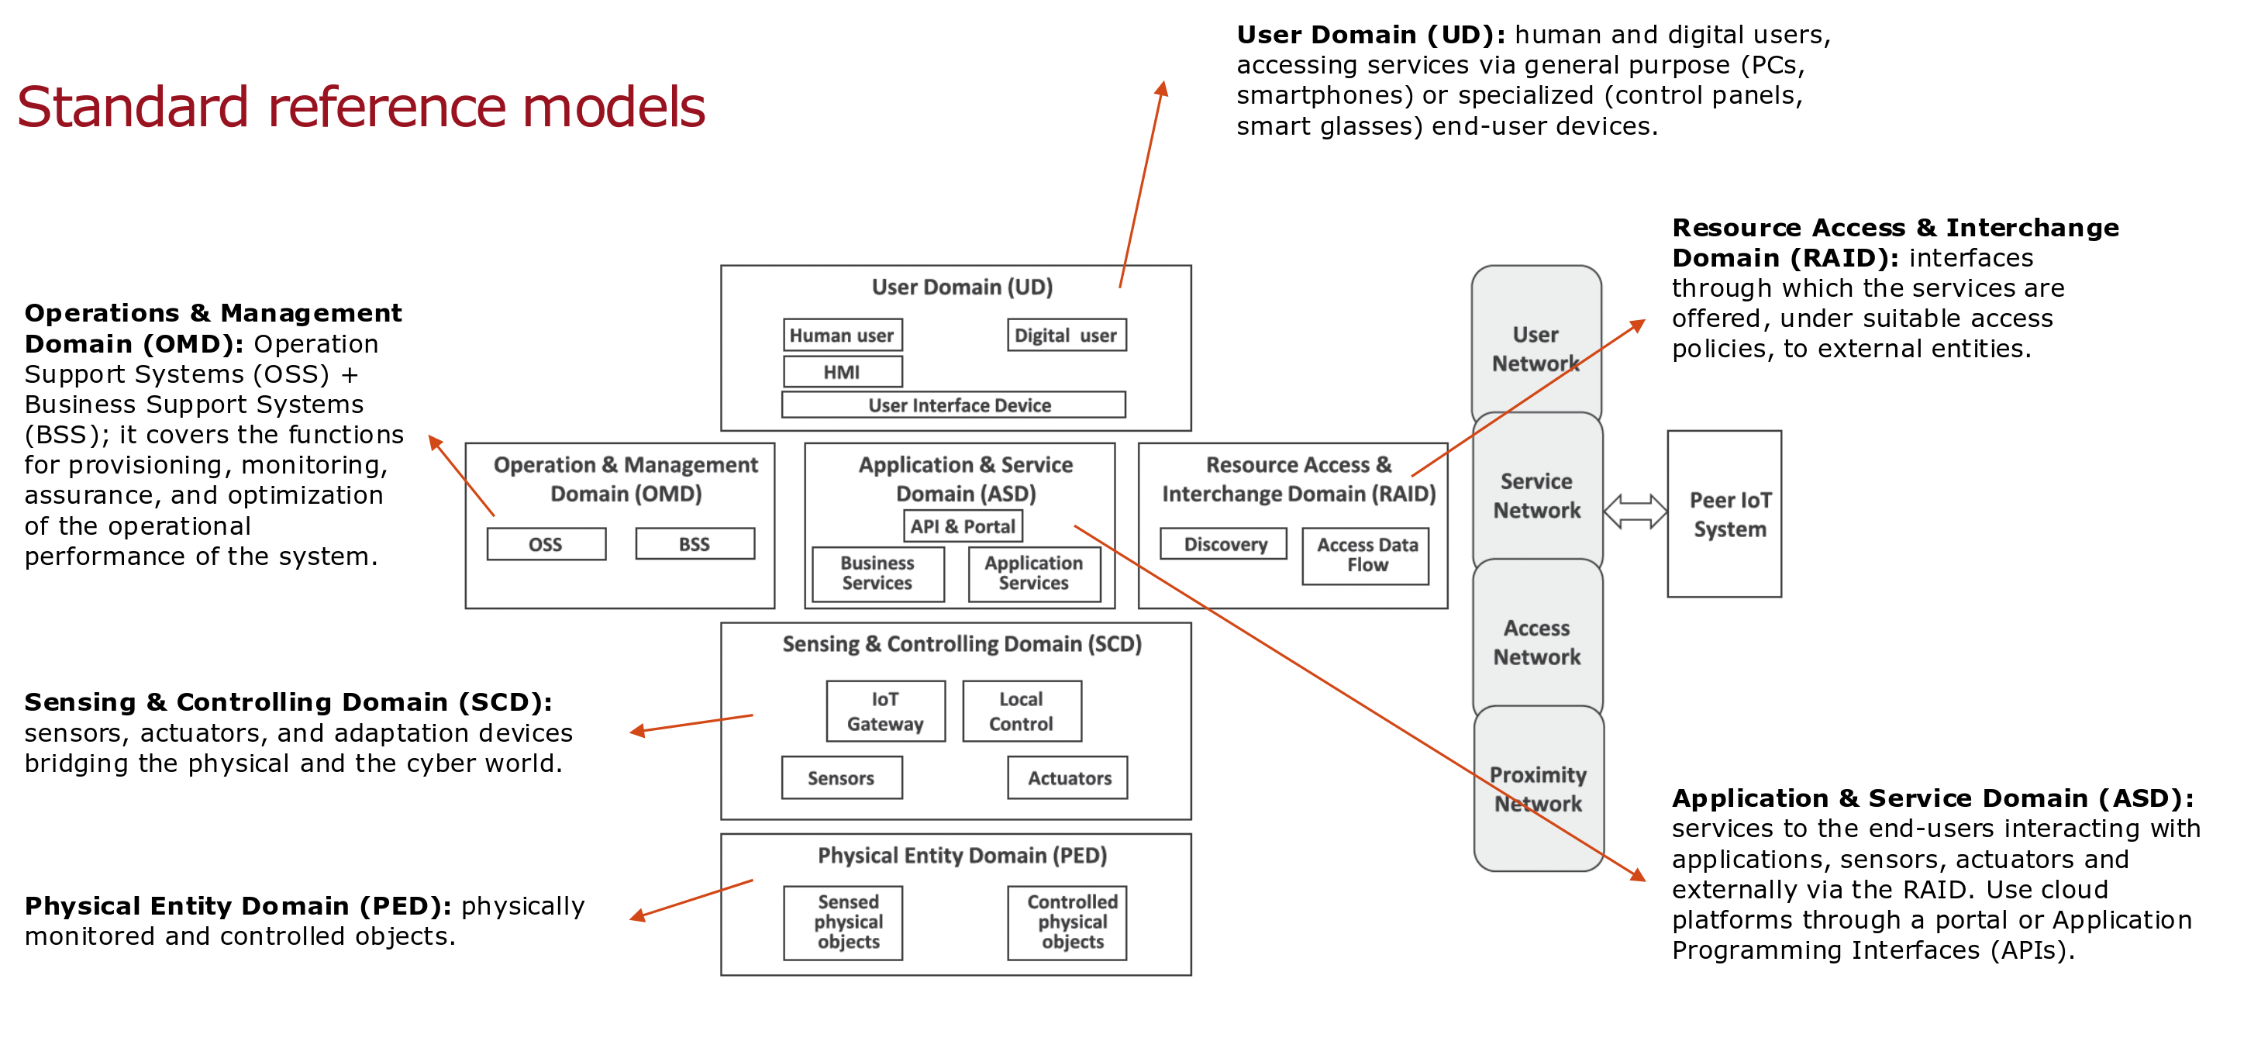
\includegraphics[width=0.8\textwidth]{Pictures/Pasted image 20251001094808.png}
\end{figure}} \\
\end{longtable}

\section{Network Architectures}\label{network-architectures}

\begin{itemize}
\tightlist
\item
  \textbf{One-level}: endpoints use full IP stack (e.g., cellular).
\item
  \textbf{Two-level (1b)}: endpoints resource-constrained, gateway
  manages protocols (LPWA, Low Power Wide Area: LoRa, SigFox, NB-IoT).
  \emph{Target of the course}
\item
  \textbf{Two-level (1c)}: endpoints support TCP/IP, traffic managed by
  router (Ethernet/Wi-Fi)
\end{itemize}

\begin{longtable}[]{@{}
  >{\raggedright\arraybackslash}p{(\linewidth - 0\tabcolsep) * \real{0.0556}}@{}}
\toprule\noalign{}
\begin{minipage}[b]{\linewidth}\raggedright
\#\# WANs - TCP/IP networks, shared among users. - Public by nature. -
\textbf{VPNs}: reserved bandwidth/security for defined groups, with
private IP addressing - Users outside of a group cannot communicate
directly with users of the group. - Use private IP addressing and
private routing protocol instances.
\end{minipage} \\
\midrule\noalign{}
\endhead
\bottomrule\noalign{}
\endlastfoot
\#\# Topologies - \textbf{Bus}: every nodes taps into a shared medium
(CSMA/CD), collisions possible. - \textbf{Ring}: token-based, eliminates
collisions, requires token management. - \textbf{Star}: master/slave,
predictable, not scalable (master bottleneck). - \textbf{Mesh}: full or
partial, robust, private, many physical links \\
\end{longtable}

\chapter{Endpoints}\label{endpoints}

\section{Sensors}\label{sensors}

\begin{itemize}
\tightlist
\item
  Devices detecting stimuli → electrical/processable output.
\item
  Types: pressure, temperature, biometric, chemical, acoustic, optical,
  positioning, etc.
\item
  Three classifications:

  \begin{itemize}
  \tightlist
  \item
    \textbf{Fixed}: stable, not moving like domotics
  \item
    \textbf{Mobile}: always moving (GPS, wearables)
  \item
    \textbf{Nomadic}: they move but then they stop somewhere else
    (portable medical devices, field sensors)
  \end{itemize}
\item
  \textbf{Active vs Passive} sensors

  \begin{itemize}
  \tightlist
  \item
    \textbf{Active}: need to run a current or send a signal to get a
    measurement (e.g., clocks, strain gauges, radar).
  \item
    \textbf{Passive}: use the physical phenomenon itself (e.g.,
    piezoaccelerometers, GPS, thermocouples).
  \end{itemize}
\end{itemize}

\subsection{Actuators}\label{actuators}

\begin{itemize}
\tightlist
\item
  Output elements performing actions.
\item
  \textbf{Digital}: on/off switching.
\item
  \textbf{Analog}: continuous signals (e.g., motor speed control).
\end{itemize}

\subsection{Gateways}\label{gateways}

\begin{itemize}
\tightlist
\item
  Bridge sensors ↔ higher-level processing/cloud.
\item
  Provide connectivity, data collection, filtering, storage, event
  processing, optional analytics
\end{itemize}

\subsection{Fog Nodes}\label{fog-nodes}

\begin{itemize}
\tightlist
\item
  ``Bring the cloud to the ground.''
\item
  More powerful than gateways, allow \textbf{local analytics with lower
  latency}.
\end{itemize}

\begin{longtable}[]{@{}
  >{\raggedleft\arraybackslash}p{(\linewidth - 0\tabcolsep) * \real{0.0556}}@{}}
\toprule\noalign{}
\begin{minipage}[b]{\linewidth}\raggedleft
\# Data plane functions \#\# Data acquisition and processing
\end{minipage} \\
\midrule\noalign{}
\endhead
\bottomrule\noalign{}
\endlastfoot
\#\#\# Sampling \\
- First, we sample: we take (regular) measurements over time, and
represent the signal with those measurements. - Nyquist theorem: if
sampling is ≥ twice as fast as the signal, sampling has no errors. -
Example: If a signal is thought to have a maximum frequency between 1000
Hz and 4000 Hz, which of the following would be the most appropriate
sample rate? - a. 500 Hz - b. 8000 Hz - c.~9000 Hz - d.~24000 Hz \\
\#\#\# Aliasing - If we do not sample ``enough,'' we have aliasing:
patterns in the sampled version. - A high frequency component in the
frequency spectrum of a signal takes the identity of a lower frequency
component in the same spectrum of the sampled signal. - This falsely
estimated signal will be indistinguishable from (i.e., be an ``alias''
to) another signal having that true lower frequency. - There are tools
to avoid this, but we need to know it is an issue. - Example: aliasing
in a sine wave.
\pandocbounded{\begin{figure}[h]
\centering
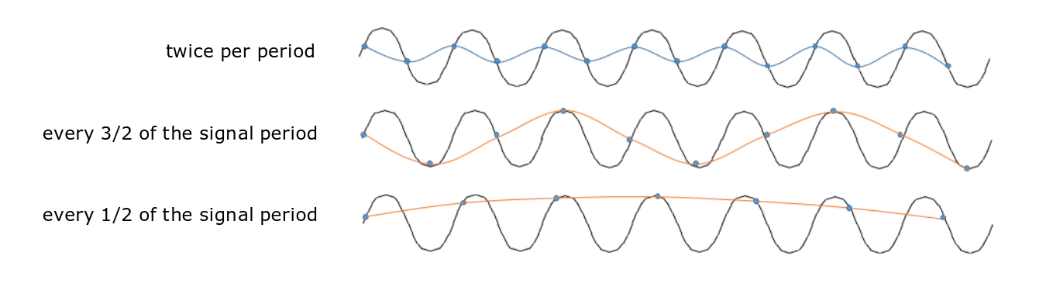
\includegraphics[width=0.8\textwidth]{Pictures/Pasted image 20251007085600.png}
\end{figure}} \\
\#\#\# Quantization - Digital values are finite: we cannot represent
continuous values precisely! - Quantization always introduces an error,
which is the sensor's natural error. - More bits, better resolution (but
more data) \\
\pandocbounded{\begin{figure}[h]
\centering
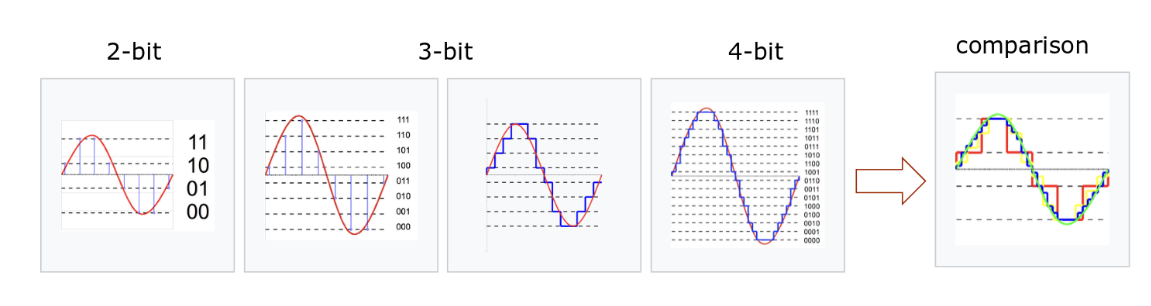
\includegraphics[width=0.8\textwidth]{Pictures/Pasted image 20251007085902.png}
\end{figure}} \\
\#\#\# Saturation - Sensors often have an upper limit, which is either
physical or dictated by the maximum quantization level: in this case, we
have saturation (all higher values are mapped to the same output) - This
is what happens when you take a picture with high exposure: all lighter
points are bright white!
\pandocbounded{\begin{figure}[h]
\centering
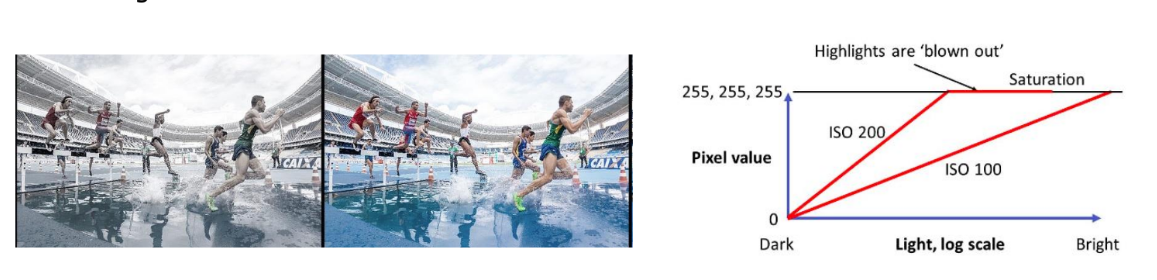
\includegraphics[width=0.8\textwidth]{Pictures/Pasted image 20251007090152.png}
\end{figure}} \\
\#\#\# Hysteresis - Sometimes sensors takes a while to track the process
because the \textbf{physical nature of the measurement is slow} - Which
means we have Hysteresis error when the delay of sensor measurements
depends on the magnitude of the change. \\
- Example: When you apply pressure to a sensor and then release that
pressure, the sensor's output should in theory return you to the same
value it started at before that specific pressure cycle. However, in
reality, there are often small differences between the initial value and
the final value after a pressure cycle. - From 0 to 100 bar - 0 bar → 0
V - 100 bar → 2500 V - 0 bar → 0.05 V - \textbf{0.02\% / 1 bar
hysteresis} \\
\#\#\# Non-linearities - Ideally, sensors should also have linear
responses: in reality, there are often non-linear effects that we need
to adjust for. \\
- Hard to predict \\
- Example: A linear sensor's output will change by equal amounts for
equal pressure changes across its entire range. - From 0 to 10 bar - 0
bar → 0 V - 10 bar → 5 V - 3 bar → 4.2 V (while I would have expected
3.75 V, according to the previous data). - \textbf{≤2\% non-linearity of
full scale} \\
\#\#\# Calibration \\
- Sensors often require calibration to give proper results: - Bias is a
constant error term in one direction. - Distortion is due to
non-linearity. \\
- By measuring a series of known quantities, we can compensate for these
issues (however, external factors such as temperature can throw off
calibration!) - Example: Using the data from the calibration sheet, we
see that the deviations are all less than the maximum deviation allowed
of 0.5\%. \\
\#\#\# Error propagation - Calculations can change the error of a
measurement, as the errors are also considered in the function you
compute. - Non-linear functions can have weird effects with measurement
errors. - Derivation (e.g., computing velocity from position
measurements) is brittle: since the measurements are close together,
noise can have a huge effect. - Integration/averaging are robust (rely
on many points, and noise is compensated). - Example: Calculating heat
index - Temperature sensor: measured (30°) with uncertainty ±0.5 -
Humidity sensor: measured (70\%) with uncertainty ±2\% (= 0.02) - Heat
index = T + 0.33×RH−0.7 = 52.4 - \textbf{Uncertainty with error
propagation: 0.828 \textgreater{} (0.5 + 0.02)} \\
\#\#\# External data communication - Sensors data may need to be shared
with external parties, such as other peer nodes at the edge, fog, and
cloud levels. - Messages exchanged between IoT nodes may be delivered
using \textbf{push} or \textbf{pull} modes. - \textbf{Pull}: a message
is explicitly requested from the source (server) by its recipient, an
IoT client. - \textbf{Push}: the data source and the gateway send data
when the specified conditions are met, such as arrival of the data
sampling time mark, or exceeding of the measurement threshold. -
\textbf{Publish/subscribe system}: data sources ``publish'' data to a
known place, and authorized clients can ``subscribe'' to data of
interest and receive related messages. - Publishers do not need to know
the identity or number of their receivers (subscribers), and the
receivers do not need to know the identity or state of their
publishers. \\
\#\#\#\# How to share sensors' data? - Some processes (e.g., an
electricity meter, a room thermostat) do not need to be sampled very
often. - If we only care about cumulative measures (how much electricity
was consumed in total), we do not need frequent samples! - On the other
hand, faster processes need frequent samples, as process can change
faster. - Why don't we transmit all the time? - There are several
reasons why we cannot transmit all the time, but we will concentrate on
two of them in this first part of the course: - Limited bandwidth -
Limited energy - Each transmission (and, in fact, each activity the
sensor performs) costs energy, as well as blocking the wireless channel
for other transmissions \\
\#\#\#\# Some solutions to send sensors' data more efficiently -
\textbf{Interpolation} - Interpolation is the mathematical tool to infer
missing data from sparse samples. We have to make some assumptions on
the nature of the process to be able to interpolate: if we have the
correct model, we can send a lot fewer data samples! - Interpolation can
also be dangerous: we can underfit (select a model that is too simple)
or overfit (select a model that is too complex and ends up following
random noise).
\pandocbounded{\begin{figure}[h]
\centering
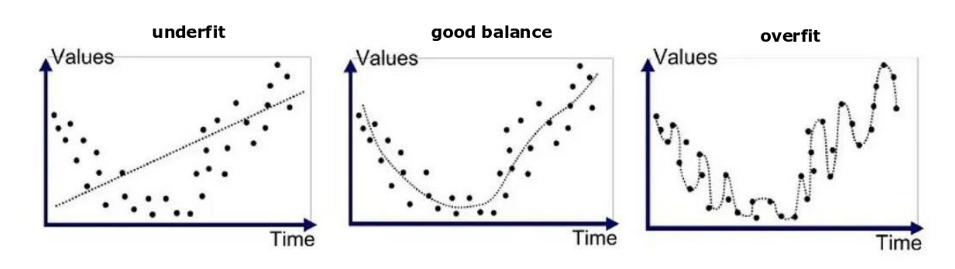
\includegraphics[width=0.8\textwidth]{Pictures/Pasted image 20251007093806.png}
\end{figure}} \\
- \textbf{Spatial correlation} - Data are usually correlated in space: -
Traffic on either side of a bridge. - Temperatures close together. -
There can be easy natural relations (points close together are similar)
or structural relations (connected points are similar). - Since
measurements have errors, correlations help us improving the quality of
estimates: we can make statistical calculations and estimates to figure
out what is happening in points (like the purple one on the bridge)
where we have no sensors, or refine our estimates. \\
- \textbf{Temporal correlation} - Data are also correlated in time: -
Traffic in one spot - Temperature measured by one sensor - The relation
here can be more or less complex, and depend on space as well (e.g.,
line at a traffic light), but we can also exploit this to get better
data with fewer transmissions. - Correlations can be misleading and
dangerous! When relying on statistical information to reconstruct
missing data or make decisions, we need to be aware that random chance
is always a possibility. \\
\end{longtable}

\subsection{Local control}\label{local-control}

\begin{itemize}
\tightlist
\item
  Provided in systems where latency is critical and/or edge autonomy is
  required.
\item
  Local control enables the edge node to execute pre-defined control
  sequences when a specified condition occurs on some combination of
  local data.
\item
  If This Then That: scenes where lights and heating/cooling are
  adjusted accordingly when users are leaving or approaching their
  homes.
\item
  \textbf{Node-RED}: provides a graphical user interface to construct
  data flows with the functional processing modules and actuation output
  stages.
\item
  In the extreme case of temperature, the script triggers the device
  shutdown.
\end{itemize}

\pandocbounded{\begin{figure}[h]
\centering
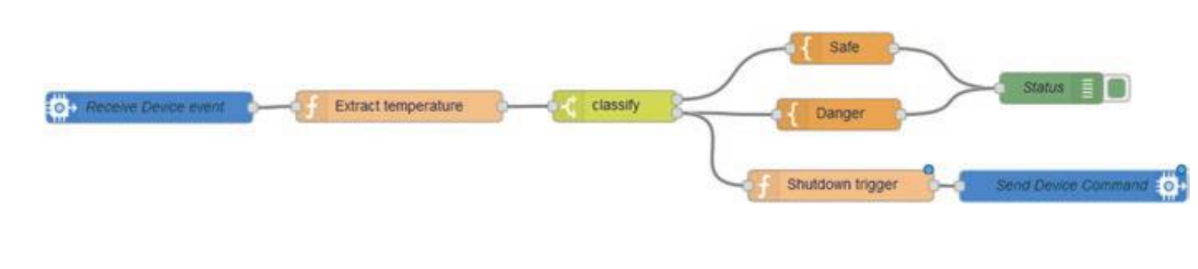
\includegraphics[width=0.8\textwidth]{Pictures/Pasted image 20251007094532.png}
\end{figure}}

\subsection{Data storage}\label{data-storage}

\begin{itemize}
\tightlist
\item
  Data storage for the acquired data may be provided by the gateway.
\item
  The existence of local storage provides the flexibility to conserve
  network bandwidth and to reduce the load on cloud resources by
  selectively reporting data that meet certain conditions.

  \begin{itemize}
  \tightlist
  \item
    \textbf{Semantic communication.}
  \item
    Depending on the nature of the physical thing being measured,
    \textbf{only some of the data points may be of interest}. E.g.,
    successive minor changes may be of little interest, but those that
    exceed a comfort guard band or change by a significant percentage or
    amount from prior readings are.
  \item
    Qualifying readings may be defined as events and reported only when
    they occur, with raw readings stored in the local database should
    they be required for auditing or subsequent analysis.
  \end{itemize}
\end{itemize}

\subsection{(Edge) analytics}\label{edge-analytics}

\begin{itemize}
\tightlist
\item
  Edge analytics for the data may be provided by the gateway or the fog
  node.
\item
  Proximity to data sources: low latency.
\item
  Ability to process high-frequency data samples (at the rate of the
  sensor) → real-time.
\item
  Conservation of network bandwidth by not sending data to the cloud.
\item
  Can operate even in disconnected mode.
\item
  Analytics generally require AI/ML models:

  \begin{itemize}
  \tightlist
  \item
    Insufficient computational resources at the edge.
  \item
    No data aggregation of edge/local data.
  \end{itemize}
\item
  IoT systems should be implemented using design tools and practices
  that facilitate flexible allocation of functions (in tandem between
  edge and cloud).
\end{itemize}

\subsection{Analytics placement}\label{analytics-placement}

\begin{itemize}
\tightlist
\item
  Optimal placement of data and processing functions is an age-old
  trade-off in distributed systems.
\item
  It is based on whether it is more cost-effective to move the data to
  the computation or to move the computation to the data, depending on:

  \begin{itemize}
  \tightlist
  \item
    Availability and cost of bandwidth
  \item
    Latency requirements for time-critical operations
  \item
    Local autonomy of operations, including disconnected mode
  \item
    Security and data control or privacy concerns
  \item
    Cost and complexity of managing distributed nodes with computing and
    storage
  \item
    Available energy resources
  \item
    Available computational capacity
  \item
    \ldots{}
  \end{itemize}
\end{itemize}

\begin{center}\rule{0.5\linewidth}{0.5pt}\end{center}

\chapter{Control plane functions}\label{control-plane-functions}

\begin{itemize}
\tightlist
\item
  Fully functional gateways may be fairly sophisticated computational
  and communications nodes that host and execute a variety of services.
\item
  They need to be properly secured and managed.
\item
  Main control functionalities:

  \begin{itemize}
  \tightlist
  \item
    Fault management (troubleshooting, error logging, and recovery).
  \item
    Remote monitoring, control, administration, and diagnostics.
  \item
    Remote firmware and software updates.
  \item
    Security updates.
  \item
    Metering (network bandwidth and software usage) and supervision.
  \item
    Provisioning and authentication.
  \end{itemize}
\end{itemize}

\begin{center}\rule{0.5\linewidth}{0.5pt}\end{center}

\subsection{(Cyber)security}\label{cybersecurity}

\begin{itemize}
\item
  The first step is to determine the security risk.
\item
  Identify, quantify, and prioritize the risks for the system, and find
  a balance between costs and potential losses from residual risks.
\item
  Model to quantify risk: vulnerability, threats, and impacts.
  \pandocbounded{\begin{figure}[h]
\centering
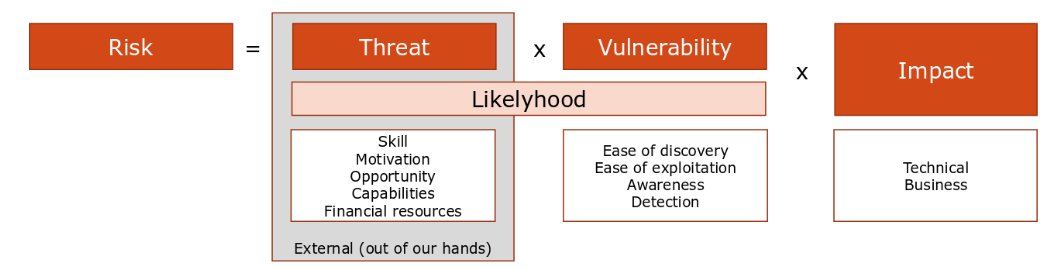
\includegraphics[width=0.8\textwidth]{Pictures/Pasted image 20251007095925.png}
\end{figure}}
\item
  \textbf{Vulnerabilities}: can originate from the design of the system
  architecture, technology, and protocols, but more often emerge in the
  implementation (e.g., coding flaws) and in the operation phases (e.g.,
  configuration errors, use of weak credential, unparched devices,
  unexpert use, etc.).
\item
  \textbf{Security measures for the diligent user}:

  \begin{itemize}
  \tightlist
  \item
    Partitioning the system into zones (characterized in terms of
    security levels).
  \item
    Adopt effective authentication protocols, tailored to the different
    zones.
  \item
    Provide cryptographic protection of data.
  \item
    Install equipment from trusted providers.
  \item
    Make and install frequent patches and workarounds (software
    updates).
  \item
    \ldots{}
  \end{itemize}
\item
  \textbf{Threat}: an IoT network is a possible point of attack if the
  endpoint is unguarded and is positioned in an easily reachable
  position.

  \begin{itemize}
  \tightlist
  \item
    \textbf{Eavesdropping}: learning confidential information.
  \item
    \textbf{Traffic analysis}: learning data origin, destination, and
    length (not the content).
  \item
    \textbf{Forgery}: building a fake message, pretending it was sent by
    someone else.
  \item
    \textbf{Masquerade}: claiming to be someone else in a single
    message.
  \item
    \textbf{Repudiation}: denying having sent or received a message.
  \item
    \textbf{Profiling}: gathering information about a single user.
  \item
    \textbf{Fingerprinting}: identifying the user associated with a
    message.
  \item
    \textbf{Jamming}: causing interference to a communication.
  \end{itemize}
\item
  \textbf{Standards}: IoT-oriented and industry-specific standards have
  been developed for security.
  \pandocbounded{\begin{figure}[h]
\centering
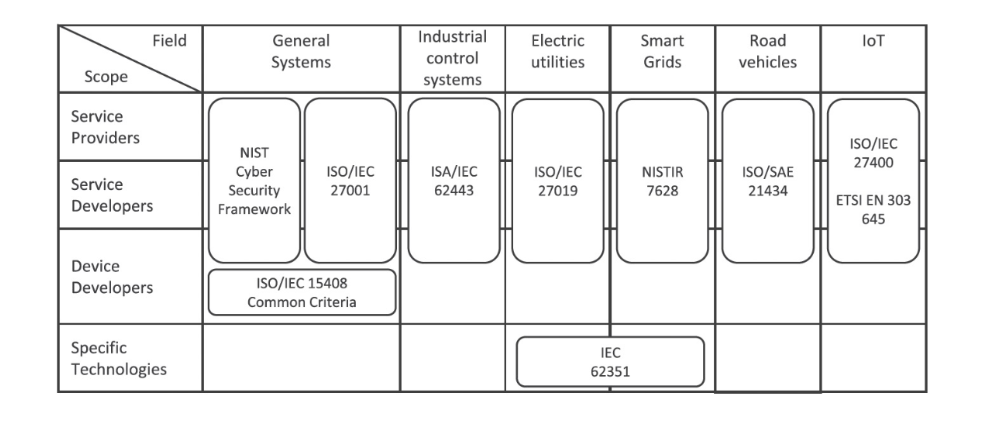
\includegraphics[width=0.8\textwidth]{Pictures/Pasted image 20251007100557.png}
\end{figure}}
\end{itemize}

\begin{longtable}[]{@{}
  >{\raggedright\arraybackslash}p{(\linewidth - 0\tabcolsep) * \real{0.0556}}@{}}
\toprule\noalign{}
\begin{minipage}[b]{\linewidth}\raggedright
\#\#\# Provisioning and authentication - \textbf{Provisioning}: the
lifecycle of an endpoint begins with its provisioning in the network. -
It is the process of giving the endpoint the configuration data and the
ability to present itself. - \textbf{Authorization}: checking the rights
of access to the network. - \textbf{Application-level authentication}:
used if the network is shared among applications. -
\textbf{Authentication}: verification of the identity (``I know your
name, is it you?''). - \textbf{Challenge-response protocol}: employs
secret keys for verification.
\end{minipage} \\
\midrule\noalign{}
\endhead
\bottomrule\noalign{}
\endlastfoot
\# QoS and performance \\
- \textbf{One-way delay (OWD)}: time between the transmission of the
first bit of a packet at an interface and the reception of the last bit
of the packet at the other interface. - Requires perfect time
synchronization between the endpoints. - \textbf{Time reference}:
Network Time Protocol (NTP). - \textbf{Two-way delay (TWD)}: time
between the transmission of the first bit of a packet at an interface
and the reception of the last bit of the packet at the same interface,
after being reflected by the system at the other end, net of the End
System Delay (ESD, processing time at the remote node). - We have that
\textbf{Round Trip Time (RTT) = TWD + ESD.} \#\# Delay -
\textbf{Packet-delay variation (PDV)} (\textasciitilde jitter): based on
previous OWD/TWD measures. - PDV = \textbar OWDi - OWDi-1\textbar{} -
PDV = \textbar OWDi - mean\{OWD\}\textbar{} - PDV = \textbar OWDi -
min\{OWD\}\textbar{} - PDV = \textbar OWDi - OWD1\textbar{} -
\ldots{} \\
- \textbf{Problem}: These delay metrics do not consider the MAC delay
(for channel access). - \textbf{End-to-end delay (E2E)}: it consists of
(at least) three components: - \textbf{MAC delay} (under the control of
the system designer). - \textbf{Access link and gateway delay} (under
the control of the system designer). - \textbf{OWD} (depends on the
WAN). \\
\#\#\# Delay and ``real-time'' - The expression \textbf{``real-time''}
may have different interpretations: - \textbf{Synchronization} to a
common time reference. - \textbf{Responding fast.} - \textbf{Responding
within predictable response times.} \\
- \textbf{Hard real-time}: if the response exceeds a limit, the system
does not operate well. - Example: respond within 5 ms - \textbf{CASE 1:}
The application always responds in 4 ms - Average delay: 4 ms; Failure
rate: 0\% - \textbf{CASE 2:} The application responds in 1 ms for 99.9\%
of the times, and in 6 ms in 0.01\%. - Average delay: 1.005 ms; Failure
rate: 10⁻³ - \textbf{Soft real-time}: it involves some response time
percentiles. \\
\#\#\# Packet loss - In an IoT network, \textbf{loss may occur} if: -
The \textbf{buffers of a node overflow.} - \textbf{Transmission errors}
(negligible in wired LANs, dominant in wireless LANs). - \textbf{Delay
much larger than expected} may be considered as a loss. \\
- How to have realistic measures of packet loss? There are some
problems: - \textbf{Long-lasting measurements:} averaging of data gives
no indications on the short period. - \textbf{Short measurements:} no
statistically meaningful data. - \textbf{Intense bursts:} too intrusive,
altering the result (not representative of a real situation). \\
\#\#\# Capacity - \textbf{Hardly a problem}, as applications are not (in
general) bandwidth demanding. - For some high-end applications (e.g.,
telemedicine, IIoT, automotive, etc.), \textbf{capacity} is generally
less important than other metrics such as reliability. -
\textbf{Example:} metering application - Collect 1M samples (or
sensors?) (of 128B) every 15 minutes. - \textbf{Average throughput:}
1,000,000 × 128B × 8 (bit) / (15 × 60) = 1.3 Mbit/s - If the same
measurements take place as unsolicited events from the endpoint in the
same second, the \textbf{link capacity} shall be around 1,000,000 × 128B
× 8 (bit) = 1 Gbit/s. \\
Those are the most important metrics, but there are other ones related
to IoT. \\
\#\#\# Reliability - \textbf{R(t)}: probability that a system is working
as expected at a certain time \emph{t.} - For most systems, the early
phase of ``high mortality'' is short and occurs during tests. - The
system is generally replaced for obsolescence as the aging phase
approaches. - In ``normal life'', most systems shall be reliable. -
\textbf{R(t)} is memoryless: the residual life of failure does not
depend on how long the system has been working → the system does not age
during ``normal life.''
\pandocbounded{\begin{figure}[h]
\centering
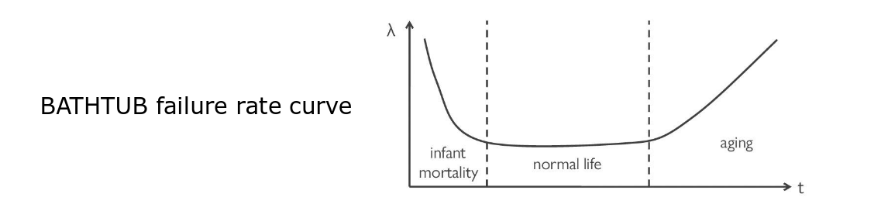
\includegraphics[width=0.8\textwidth]{Pictures/Pasted image 20251008085321.png}
\end{figure}} \\
\#\#\# Availability - \textbf{Probability that the system is working}
when observed at a random time instant. - We assume that the system can
be periodically repaired if needed and put back in service. -
\textbf{Mean Time Between Failures (MTBF).} - \textbf{Mean Time To
Repair (MTTR).} \\
\(
A = \frac{MTBF}{MTBF + MTBR}
\)
\pandocbounded{\begin{figure}[h]
\centering
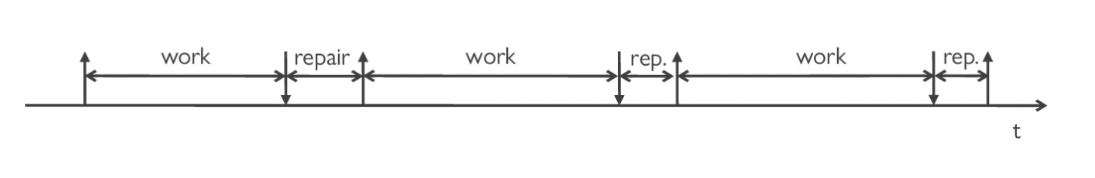
\includegraphics[width=0.8\textwidth]{Pictures/Pasted image 20251008085509.png}
\end{figure}} \\
\#\#\#\# Availability (example) - For memoryless systems, \textbf{MTBF =
Mean Time To Fail (MTTF) = 1/λ.} \\
- \textbf{Example:} prevention of fires in a forest - \emph{N} sensors
that monitor fires in the forest. - Sensors fail at rate \textbf{λ.} -
The prevention works if \emph{x\%} of sensors are active and alive. -
Period of effectiveness of the system (\textbf{T}): \(
N e^{-\lambda T} = xN \quad \Rightarrow \quad T = \frac{-\ln x}{\lambda}
\) \\
\end{longtable}

\chapter{Energy constraints}\label{energy-constraints}

\section{Introduction}\label{introduction}

\begin{itemize}
\tightlist
\item
  Most sensors and components use electrical energy, i.e., they exploit
  the movements of electrons across a conducting medium.\\
\item
  Powering is a very important issue, and depends on the endpoint
  capabilities and the network architecture procedures.
\end{itemize}

\begin{longtable}[]{@{}
  >{\raggedright\arraybackslash}p{(\linewidth - 2\tabcolsep) * \real{0.5000}}
  >{\raggedright\arraybackslash}p{(\linewidth - 2\tabcolsep) * \real{0.5000}}@{}}
\toprule\noalign{}
\begin{minipage}[b]{\linewidth}\raggedright
Type
\end{minipage} & \begin{minipage}[b]{\linewidth}\raggedright
Examples
\end{minipage} \\
\midrule\noalign{}
\endhead
\bottomrule\noalign{}
\endlastfoot
\textbf{Mains / manually recharged} & Field buses Smartphones Smart grid
devices \\
\textbf{Battery} & Most sensors \\
\textbf{Data line} & Videocameras \\
\textbf{Harvesting} & Environmental sensors \\
\end{longtable}

\begin{longtable}[]{@{}
  >{\raggedright\arraybackslash}p{(\linewidth - 0\tabcolsep) * \real{0.0556}}@{}}
\toprule\noalign{}
\begin{minipage}[b]{\linewidth}\raggedright
\#\# Sources of consumption \#\#\# Computing
\end{minipage} \\
\midrule\noalign{}
\endhead
\bottomrule\noalign{}
\endlastfoot
\#\#\# Boards and PLCs - Boards and PLCs are standard circuits used in
industrial automation. Larger IoT nodes also use Arduinos or other
pre-made boards. - Smaller, more efficient nodes are often designed ad
hoc, to use as little energy as possible. In general, IoT nodes have
limited computational capabilities. \\
\textbf{Example: Arduino-UNO} The Arduino Uno is a microcontroller board
based on the ATmega328. It contains everything needed to support the
microcontroller; simply connect it to a computer with a USB cable or
power it with an AC-to-DC adapter or battery to get started. \\
\end{longtable}

\subsection{Communication}\label{communication}

\begin{itemize}
\tightlist
\item
  Digital communication usually requires more steps than just sending a
  wave, and each consumes energy:\\
\end{itemize}

\begin{enumerate}
\def\labelenumi{\arabic{enumi}.}
\tightlist
\item
  \textbf{Encoding and error protection.}

  \begin{itemize}
  \tightlist
  \item
    Use known redundant codes: the simplest example is the parity check
    bit.
  \item
    Decoders are often complex, but can correct errors in transmission
    and recover the original packet. However, complexity is paid for in
    energy.
  \end{itemize}
\item
  \textbf{Preambles for synchronization and channel estimation.}
\item
  \textbf{Modulation} from the baseband digital signal to the passband
  analog signal.
\item
  \textbf{Transmission} (power is applied to the antenna) (not required
  for reception).

  \begin{itemize}
  \tightlist
  \item
    IoT transmissions are usually slow (low bitrate), but distance plays
    a large role.
  \end{itemize}
\end{enumerate}

\begin{longtable}[]{@{}
  >{\raggedright\arraybackslash}p{(\linewidth - 0\tabcolsep) * \real{0.0556}}@{}}
\toprule\noalign{}
\endhead
\bottomrule\noalign{}
\endlastfoot
\#\# Source of energy \#\#\# Mains power - Provide virtually unlimited
power, making it possible to employ complex protocols, work at high
bitrates, and achieve long-distance communication. - There are some
drawbacks: - Only work in wired fixed systems. - Can be dangerous in
environments at risk of fire and explosions. - Need to lay out an
electric line (challenging in hard-to-reach remote/rural areas). - Need
to put transformers (expensive). \\
\end{longtable}

\subsection{Power over Ethernet (PoE)}\label{power-over-ethernet-poe}

\begin{itemize}
\tightlist
\item
  Employ the wired communication infrastructure also for powering.
\item
  Can carry DC power on the twisted pair used for Ethernet connectivity.
\item
  Only one cabled infrastructure needs to be in place.
\item
  Transformers are not needed.
\end{itemize}

\begin{center}\rule{0.5\linewidth}{0.5pt}\end{center}

\subsection{Powerline communication}\label{powerline-communication}

\begin{itemize}
\tightlist
\item
  It is the opposite of PoE.
\item
  Use the powerline to carry data.
\item
  Based on modulation between high-frequency data and low-frequency
  electricity.
\item
  Only one cabled infrastructure needs to be in place.
\item
  Advantageous when the system to be monitored and controlled is the
  power grid itself.
  \pandocbounded{\begin{figure}[h]
\centering
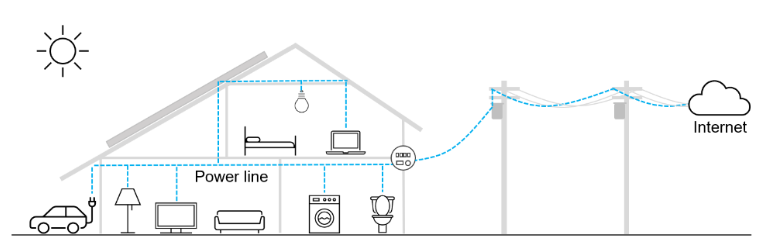
\includegraphics[width=0.8\textwidth]{Pictures/Pasted image 20251008091052.png}
\end{figure}}
\end{itemize}

\begin{longtable}[]{@{}
  >{\raggedright\arraybackslash}p{(\linewidth - 0\tabcolsep) * \real{0.0556}}@{}}
\toprule\noalign{}
\begin{minipage}[b]{\linewidth}\raggedright
\#\#\# Batteries - Batteries use the charge difference between ions to
induce a potential difference. - \textbf{Rechargeable} batteries can run
the circuit backwards and move the electrons back (by connecting a
stronger generator). - Charging is never perfect: chemical impurities
build up. - If the battery runs out completely, it is often impossible
to recharge without direct intervention (which may be expensive): the
objective is \textbf{never to let it run out!} - Apply
\textbf{statistical data} and direct information from the meter to
define a plan of \textbf{proactive} on-field \textbf{intervention} if
needed → carry out with proper timing to minimize the number of
substitutions in the lifetime and the number of dedicated ``truck
rolls'' or manual readings.
\end{minipage} \\
\midrule\noalign{}
\endhead
\bottomrule\noalign{}
\endlastfoot
\#\#\# Energy harvesting - Energy harvesting: recharge it while it is
running. - Energy harvesting sensors and actuators are equipped with
some kind of generator and can recharge their battery from it. This
allows them to stay alive much longer than with a single battery charge,
even if they get very little energy.
\pandocbounded{\begin{figure}[h]
\centering
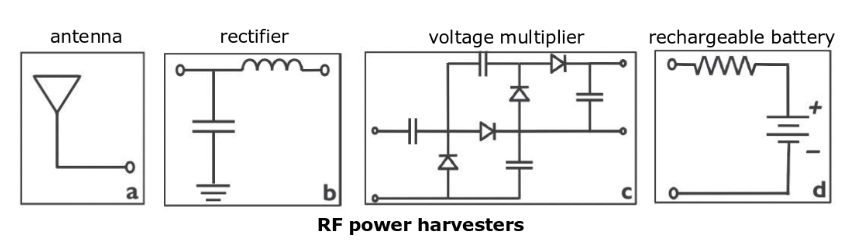
\includegraphics[width=0.8\textwidth]{Pictures/Pasted image 20251008091530.png}
\end{figure}} \\
\end{longtable}

\subsection{Solar and wind energy}\label{solar-and-wind-energy}

\begin{itemize}
\tightlist
\item
  \textbf{Solar panels} are now cheap, and solar energy is renewable and
  clean.

  \begin{itemize}
  \tightlist
  \item
    The sensor needs to be exposed (shade can be a problem, underground
    or indoor sensors will not work).
  \item
    Photovoltaic cells will not generate any power at night (the sensor
    needs to get through the night on a single charge).
  \end{itemize}
\item
  Another possibility is wind energy, but there are several challenges:

  \begin{itemize}
  \tightlist
  \item
    The sensor still needs to be exposed (underground or indoor sensors
    will not work).
  \item
    Wind is intermittent and unpredictable.
  \item
    Small turbines are inefficient.
  \end{itemize}
\end{itemize}

\begin{longtable}[]{@{}
  >{\raggedright\arraybackslash}p{(\linewidth - 0\tabcolsep) * \real{0.0556}}@{}}
\toprule\noalign{}
\begin{minipage}[b]{\linewidth}\raggedright
\#\#\# Thermal and vibration energy - \textbf{Thermal energy} is cheap
when the sensor has access to temperature gradients: - The
inside/outside or ground/air gradient can generate energy. - The power
is usually very small, but may be the only option for buried sensors. -
Need for long distances between terminals. - Good for wearables: the
difference between body temperature and the air is high. - Vibration
energy can be collected using piezoelectric devices with good
efficiency. - The constant presence of vibrations energetic enough to
power the endpoint is uncertain, except in some industrial environments.
\end{minipage} \\
\midrule\noalign{}
\endhead
\bottomrule\noalign{}
\endlastfoot
\#\#\# Wireless power transfer (WPT) - Sensors can benefit from the
power of received transmissions, but the benefits are tiny at longer
distances: this is only feasible for very low-power sensors. -
\textbf{Inductive coupling}: uses electromagnetic fields to transfer
energy between coils. - \textbf{Capacitive coupling}: transfers energy
via electric fields between conductive plates. - Uses \textbf{RF
signals} to transfer power over longer distances (several meters to
kilometers). - Uses \textbf{focused laser beams} to transmit power over
long distances. \\
\end{longtable}

\subsection{Passive sensors}\label{passive-sensors}

\begin{itemize}
\tightlist
\item
  We can also use the received transmission to power the circuit
  directly: \textbf{RFID tags, biometric passports, and contactless
  cards} work this way.
\item
  Power loss is huge: these only work over short distances.
\item
  The sensor cannot actively transmit or record data, only respond to
  messages.
\item
  There are \textbf{privacy issues} (anyone can read a tag, the only
  limit is the SNR).
  \pandocbounded{\begin{figure}[h]
\centering
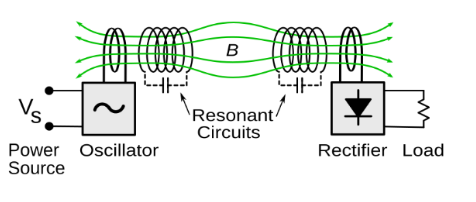
\includegraphics[width=0.8\textwidth]{Pictures/Pasted image 20251008091951.png}
\end{figure}}
\end{itemize}


% --- Chapter from 04. Radio Frequency IDentification (RFID).md ---
\subsection{Spectrum}\label{spectrum}

\begin{itemize}
\item
  Spectrum is a limited resource (interference, collision, etc.).
\item
  Necessary measures to ensure efficient and fair use of this resource.
\item
  Controlled and owned by the State, that is responsible to provide
  geography-based regulations for the use of the spectrum.
  \pandocbounded{\begin{figure}[h]
\centering
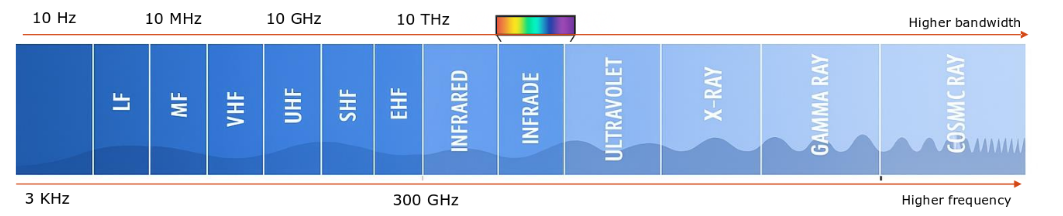
\includegraphics[width=0.8\textwidth]{Pictures/Pasted image 20251008083816.png}
\end{figure}}
\item
  \textbf{Licensed spectrum}: allocation of spectrum resources to
  private companies (e.g., cellular network operators) upon concession
  fees (auctions).

  \begin{itemize}
  \tightlist
  \item
    In Italy, 5G spectrum auction in 2018: 6.5 B€
    \url{https://www.corrierecomunicazioni.it/telco/5g/chiusa-lasta-5g-incasso-oltre-i-65-miliardi/}
  \item
    It provides the best quality of service for end customers.
  \end{itemize}
\item
  \textbf{Unlicensed spectrum}: free access to spectrum without any
  centralized control.

  \begin{itemize}
  \tightlist
  \item
    \emph{Unlicensed does not mean unregulated.}
  \end{itemize}
\item
  \textbf{``Reserved'' spectrum}: for public safety, emergency forces,
  police, military, \ldots{}
\end{itemize}

\begin{longtable}[]{@{}
  >{\raggedright\arraybackslash}p{(\linewidth - 0\tabcolsep) * \real{0.0556}}@{}}
\toprule\noalign{}
\endhead
\bottomrule\noalign{}
\endlastfoot
\#\#\#\# Licensed spectrum (examples) \\
- Spectrum allocation in the US (from 300 MHz to 3 GHz):
\url{https://www.ntia.doc.gov/files/ntia/publications/2003-allochrt.pdf}
- 4G LTE LICENSED frequency bands in Italy:
\url{https://www.sqimway.com/lte_band.php} \\
\end{longtable}

\subsubsection{Unlicensed spectrum}\label{unlicensed-spectrum}

\begin{itemize}
\tightlist
\item
  Also referred to as \textbf{Instrumental, Scientific, and Medical
  (ISM)} bands.
\item
  It is available to any number of customers, but with no exclusive
  rights.
\item
  \textbf{Target:} applications which are not lucrative enough to
  justify the cost of licence, but prove valuable if considered
  collectively.

  \begin{itemize}
  \tightlist
  \item
    Notable examples: \textbf{Wi-Fi}, \textbf{Bluetooth}, etc.
  \end{itemize}
\item
  \textbf{Unlicensed does not mean unregulated} → there are still some
  rules to avoid/minimize interference, and to promote fair use of
  resources.

  \begin{itemize}
  \tightlist
  \item
    Some regulation mechanisms: \textbf{ERP limits}, \textbf{LBT},
    \textbf{duty cycle}, etc.
  \item
    Regulations are not necessarily aligned in all the Regions of the
    world, but there are some levels of superimposition (e.g.,
    \textbf{2.4 GHz ISM band} for Wi-Fi).
  \end{itemize}
\end{itemize}

\begin{center}\rule{0.5\linewidth}{0.5pt}\end{center}

\subsubsection{Unlicensed spectrum in Europe:
ERP}\label{unlicensed-spectrum-in-europe-erp}

\begin{itemize}
\tightlist
\item
  At the European level, spectrum is regulated by the \textbf{European
  Commission (EC)}, \textbf{Electronic Communications Committee (ECC)},
  and the \textbf{European Telecommunications Standard Institute
  (ETSI)}.
\item
  Different rules/limitations are defined.
\item
  \textbf{Effective Radiated Power (ERP):} it evaluates the emissions of
  a device.
\item
  It is related to the \textbf{Effective Isotropic Radiated Power
  (EIRP)}, defined as the power that would have to be used on an
  isotropic antenna in order to get the same field strength that the
  tested device produces at the same distance.
\item
  We have that \textbf{ERP = EIRP -- 2.15.}
\end{itemize}

\begin{center}\rule{0.5\linewidth}{0.5pt}\end{center}

\subsubsection{Unlicensed spectrum in Europe:
LBT}\label{unlicensed-spectrum-in-europe-lbt}

\begin{itemize}
\tightlist
\item
  \textbf{Listen Before Talk (LBT):} a radio transmitter first senses
  its radio environment before it starts a transmission.
\item
  The device continuously monitors channels to transmit only when a
  channel is not in use.
\item
  For a device to transmit its data (talk), it needs to ensure that the
  channel is free (listen).
\item
  \textbf{How to monitor/sense the channel?}

  \begin{itemize}
  \tightlist
  \item
    \textbf{Energy detection:} The receiver measures the received power
    in the band of interest over a sensing interval. If the measured
    energy exceeds a predefined threshold, the channel is considered
    busy.\\
  \item
    \textbf{Layer-2 frame decoding:} The receiver tries to detect and
    decode known structures in the frame. If a valid preamble or header
    is detected, the channel is declared busy.
  \end{itemize}
\end{itemize}

\begin{center}\rule{0.5\linewidth}{0.5pt}\end{center}

\subsubsection{Unlicensed spectrum in Europe:
DC}\label{unlicensed-spectrum-in-europe-dc}

\begin{itemize}
\tightlist
\item
  \textbf{Duty Cycle (DC):} it is defined as the ratio, expressed as a
  percentage, of the maximum transmitter ``on'' time over one hour,
  relative to a one hour period.
\item
  These limitations apply to every receiver, excluding those with LBT
  capabilities.
\item
  \textbf{1\% DC:} the max. transmission time of any device is 1\% of an
  hour (i.e., 36 seconds in an hour).
\end{itemize}

\pandocbounded{\begin{figure}[h]
\centering
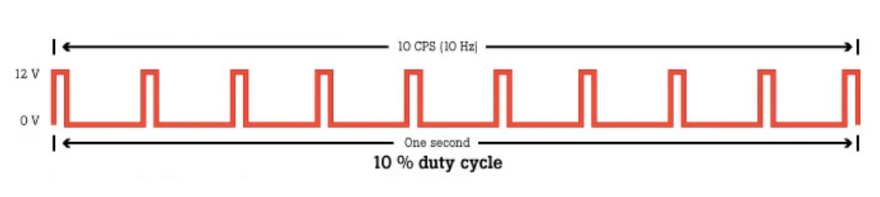
\includegraphics[width=0.8\textwidth]{Pictures/Pasted image 20251008100150.png}
\end{figure}}

\begin{center}\rule{0.5\linewidth}{0.5pt}\end{center}

\subsubsection{Unlicensed spectrum in
Europe}\label{unlicensed-spectrum-in-europe}

\begin{itemize}
\tightlist
\item
  Some of the most important ISM sub-bands in Europe (focus on IoT use
  cases).
\item
  Country specific.
\end{itemize}

\begin{longtable}[]{@{}
  >{\raggedright\arraybackslash}p{(\linewidth - 8\tabcolsep) * \real{0.1103}}
  >{\raggedright\arraybackslash}p{(\linewidth - 8\tabcolsep) * \real{0.2206}}
  >{\raggedright\arraybackslash}p{(\linewidth - 8\tabcolsep) * \real{0.2353}}
  >{\raggedright\arraybackslash}p{(\linewidth - 8\tabcolsep) * \real{0.1176}}
  >{\raggedright\arraybackslash}p{(\linewidth - 8\tabcolsep) * \real{0.3162}}@{}}
\toprule\noalign{}
\begin{minipage}[b]{\linewidth}\raggedright
Range {[}MHz{]}
\end{minipage} & \begin{minipage}[b]{\linewidth}\raggedright
Max. power
\end{minipage} & \begin{minipage}[b]{\linewidth}\raggedright
Duty cycle
\end{minipage} & \begin{minipage}[b]{\linewidth}\raggedright
Example
\end{minipage} & \begin{minipage}[b]{\linewidth}\raggedright
Example IoT scenario
\end{minipage} \\
\midrule\noalign{}
\endhead
\bottomrule\noalign{}
\endlastfoot
169.4--169.8125 & 10 mW / 500 mW (169.4--169.475) & 1\% or 0.1\% / 10\%
(169.4--169.475) & Wireless M-Bus & Water and gas metering \\
433.050--434.790 & 10 mW & 10\% & RFID, NFC & Metering \\
==863--870== & ==25 mW / 500 mW (869.4--869.650)== & ==1\% or 0.1\% /
10\% (869.4--869.650)== & ==LoRa, Zigbee== & ==Metering, Smart city,
environmental control== \\
==2400--2483.5== & ==100 mW== & ==N/A== & ==Bluetooth, Wi-Fi== & ==Smart
home== \\
5150--5350 & 200 mW & Transmission power control & Wi-Fi (802.11) &
Smart home \\
5470--5725 & 1000 mW & Transmission power control & Wi-Fi (802.11) &
Smart home \\
\end{longtable}

\begin{center}\rule{0.5\linewidth}{0.5pt}\end{center}

\subsection{Short-range}\label{short-range}

\subsubsection{Introduction}\label{introduction}

\begin{itemize}
\tightlist
\item
  \textbf{Short-range:} (generally) cell diameter smaller than 100 m.
\item
  Does not support mobility/handover.
\item
  Can be classified according to the reach of the radio link:

  \begin{itemize}
  \tightlist
  \item
    \textbf{Vicinity and proximity networks}, from a few cm to
    \textasciitilde2--3 m.
  \item
    \textbf{Wireless Personal Area Networks (WPANs)}, up to
    \textasciitilde10 m.
  \item
    \textbf{Wireless Local Area Networks (WLANs)}, up to
    \textasciitilde100 m.
  \end{itemize}
\item
  Are sometimes referred to as \textbf{Low-Rate WPAN.}
  \pandocbounded{\begin{figure}[h]
\centering
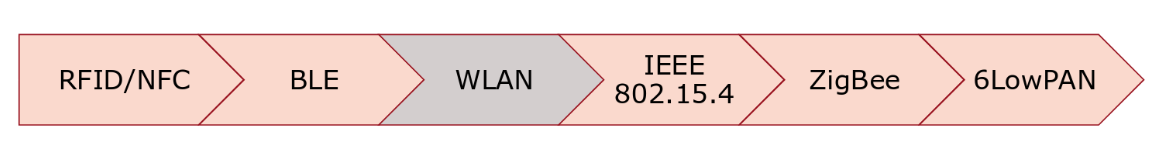
\includegraphics[width=0.8\textwidth]{Pictures/Pasted image 20251008100547.png}
\end{figure}}
\end{itemize}

\begin{longtable}[]{@{}
  >{\raggedright\arraybackslash}p{(\linewidth - 0\tabcolsep) * \real{0.0556}}@{}}
\toprule\noalign{}
\endhead
\bottomrule\noalign{}
\endlastfoot
\# Radio Frequency: IDentification (RFID) and NFC \\
\#\# RFID \\
\#\#\# Overview Radio Frequency Identification (RFID) is a method for
remotely storing and retrieving data through \textbf{RFID tags} and
\textbf{readers}. Tags store information that readers can access
wirelessly and automatically. Tags can be \textbf{WORM (Write Once Read
Many)} or \textbf{rewritable}, and may integrate other sensors.
Advantages include no line-of-sight requirement and automated data
exchange. However, privacy concerns exist regarding data tracking and
misuse. \\
\end{longtable}

\subsection{How It Works}\label{how-it-works}

RFID tags have embedded chips storing information that can be
rewritten.\\
When a reader emits a radio signal, the \textbf{tag's coil} couples
inductively with the reader's coil, transferring energy (a form of
\textbf{wireless power transfer}).\\
The tag uses this energy to respond, enabling data exchange over
variable distances.
\pandocbounded{\begin{figure}[h]
\centering
\fbox{Missing Image: Pasted image 20251014084153.png}
\end{figure}}
https://youtu.be/-Wf7aadxBkE?si=e7GMOLnfuQ8he80f

\begin{center}\rule{0.5\linewidth}{0.5pt}\end{center}

\subsection{Near-field Coupling}\label{near-field-coupling}

The coupling between tag and reader happens in the \textbf{near-field
region}, meaning the distance must be much smaller than the signal
wavelength (≈15\% of it).\\
Operating at lower frequencies increases the wavelength, thus expanding
the working distance: - At \textbf{2.4 GHz}, λ ≈ 0.13 m → range ≈ 20
cm\\
- At \textbf{13.56 MHz}, λ ≈ 22 m → range ≈ 3 m

\begin{center}\rule{0.5\linewidth}{0.5pt}\end{center}

\subsection{Tags Visualized}\label{tags-visualized}

\pandocbounded{\begin{figure}[h]
\centering
\fbox{Missing Image: Pasted image 20251014085031.png}
\end{figure}}
RFID tags typically include an \textbf{antenna} and an
\textbf{integrated circuit (chip)}.\\
The antenna captures electromagnetic energy from the reader, while the
chip stores and processes information.\\
Different tag designs exist depending on frequency range, application,
and power type (active, semi-passive, passive).

\begin{center}\rule{0.5\linewidth}{0.5pt}\end{center}

\subsection{Applications}\label{applications}

RFID systems are widely used for: - \textbf{Security}: identification
cards, passports\\
- \textbf{Access control}: Telepass, metro cards\\
- \textbf{Retail and logistics}: tracking merchandise, inventory, pallet
management\\
- \textbf{Ticketing and sports}: electronic ticket systems, race
tracking\\
- \textbf{NFC in smartphones}: contactless interactions

Readers can monitor entries/exits or track specific tagged items for
process monitoring.

\begin{center}\rule{0.5\linewidth}{0.5pt}\end{center}

\subsection{Applications: Passport}\label{applications-passport}

Since 2006, \textbf{RFID tags have been embedded in British and U.S.
passports}.\\
They store printed information (including a \textbf{digital photograph})
and consist of: - A \textbf{microchip} containing personal data\\
- A \textbf{tag antenna} for communication\\
- A \textbf{substrate} to hold components together\\
These \textbf{biometric passports} allow for faster and more secure
identity verification.

\begin{center}\rule{0.5\linewidth}{0.5pt}\end{center}

\subsection{Applications: Metro Card}\label{applications-metro-card}

Metro systems use \textbf{RFID cards} to manage balances securely
through cryptographic protection.\\
When a passenger enters or exits a station, the reader updates the card
balance locally: - \textbf{Entry:} records time and station\\
- \textbf{Exit:} calculates fare and updates balance\\
Readers periodically sync with a central server for auditing, lost card
tracking, and balance verification.\\
Users can also check balances online.

\begin{center}\rule{0.5\linewidth}{0.5pt}\end{center}

\subsection{Applications: Merchandise in Stores
(1/3)}\label{applications-merchandise-in-stores-13}

RFID tags in retail enable: - \textbf{Data storage:} more information
than barcodes, editable anytime\\
- \textbf{Quality control:} tracking goods from production to storage\\
- \textbf{Speed:} read multiple tags simultaneously at a distance\\
- \textbf{Inventory management:} automatic product location and stock
updates\\
- \textbf{Durability:} resistant to handling and environmental stress

Common example: \textbf{clothing RFID tags}.

\begin{center}\rule{0.5\linewidth}{0.5pt}\end{center}

\subsection{Applications: Merchandise in Stores
(2/3)}\label{applications-merchandise-in-stores-23}

RFID supports \textbf{anti-theft} and \textbf{authenticity
verification}.\\
When an unpaid item passes through security gates: - The
\textbf{transmitter}'s radio waves induce a current in the tag's
antenna. - The tag emits a secondary signal at a specific frequency. -
The \textbf{receiver} detects this and triggers an alarm.

\textbf{Note:} Security gates are tall to enhance detection field
coverage.

\begin{longtable}[]{@{}
  >{\raggedright\arraybackslash}p{(\linewidth - 0\tabcolsep) * \real{0.0556}}@{}}
\toprule\noalign{}
\endhead
\bottomrule\noalign{}
\endlastfoot
\#\#\# Applications: Merchandise in Stores (3/3) At checkout,
\textbf{RFID tags are deactivated} to prevent theft or false alarms. A
\textbf{deactivation pad} disables the electronic components in the tag,
ensuring they no longer emit signals when exiting the store. This system
reduces human error and enhances automatic theft prevention.
\pandocbounded{\begin{figure}[h]
\centering
\fbox{Missing Image: Pasted image 20251014085939.png}
\end{figure}}
- Tall for work in small proximity - EAS systems use \textbf{inductive
or resonant antennas}, which form a field that depends on coil size and
geometry. The \textbf{larger the antenna}, the more uniform and ``deep''
the detection zone can be across a wide doorway. - Tall vertical
antennas give: - better sensitivity at the top and bottom, - less dead
zone near the middle, - higher signal-to-noise ratio. \\
\end{longtable}

\subsection{RFID vs.~Barcode}\label{rfid-vs.-barcode}

\begin{longtable}[]{@{}lll@{}}
\toprule\noalign{}
Feature & RFID & Barcode \\
\midrule\noalign{}
\endhead
\bottomrule\noalign{}
\endlastfoot
Rate & Thousands simultaneously & One at a time \\
Range & Up to a few meters & \textasciitilde6 meters \\
Speed & Very fast (milliseconds) & Slow \\
Line-of-sight & Not required & Required \\
Identification & Unique per item & Item type only \\
\end{longtable}

RFID is thus superior for automation, scalability, and inventory
tracking.

\begin{center}\rule{0.5\linewidth}{0.5pt}\end{center}

\subsection{Electronic Product Code
(EPC)}\label{electronic-product-code-epc}

The \textbf{EPCGlobal} consortium (founded in 2003) standardized RFID
operation.\\
The \textbf{Electronic Product Code (EPC)} uniquely identifies any
physical object across the world.\\
Key aspects: - Encodes product and manufacturer info. - Accessible
through \textbf{EPC Information Services (EPCIS)} via \textbf{web
services} (SOAP, WSDL). - Enables global traceability for logistics and
retail applications.

\begin{longtable}[]{@{}
  >{\raggedright\arraybackslash}p{(\linewidth - 0\tabcolsep) * \real{0.0556}}@{}}
\toprule\noalign{}
\endhead
\bottomrule\noalign{}
\endlastfoot
\#\#\# Electronic Product Code (EPC) Structure The EPC is composed of
several fields: - \textbf{Header (8 bits):} defines the partitioning
scheme (up to 256 instances) - \textbf{EPC Manager (28 bits):}
manufacturer ID (\textgreater268 million instances) - \textbf{Object
Class (24 bits):} product type (\textgreater16 million instances) -
\textbf{Serial Number (36 bits):} unique identifier for each item
(\textgreater68 billion instances) \\
This structure guarantees a \textbf{globally unique ID} for every item,
across all manufacturers and time. \\
\end{longtable}

\subsection{Types of Tag}\label{types-of-tag}

RFID tags differ by \textbf{power source} and \textbf{functionality}: -
\textbf{Semi-passive:} contain a small battery activated by reader
signals; typical lifespan 3--5 years. Used in temperature or
environmental sensors.\\
- \textbf{Active:} have a dedicated battery for continuous transmission,
allowing \textbf{longer range} and \textbf{richer data} (e.g., Telepass,
asset tracking, personnel tags).

Applications include \textbf{cold-chain logistics}, \textbf{warehouse
monitoring}, and \textbf{vehicle tracking}.

\begin{center}\rule{0.5\linewidth}{0.5pt}\end{center}

\subsection{Active Tag: Telepass}\label{active-tag-telepass}

Telepass uses \textbf{Active RFID} at around \textbf{5.8 GHz} (microwave
frequency).\\
When the vehicle enters a toll gate: 1. Roadside sensors emit a
microwave signal to wake nearby devices.\\
2. The in-car transponder activates and sends its \textbf{unique ID}.\\
3. The system verifies the ID in the database and opens the barrier if
authorized.

Active RFID ensures \textbf{fast, reliable, and long-distance}
communication.

\begin{longtable}[]{@{}
  >{\raggedright\arraybackslash}p{(\linewidth - 0\tabcolsep) * \real{0.0556}}@{}}
\toprule\noalign{}
\endhead
\bottomrule\noalign{}
\endlastfoot
\#\#\# Types of Tag (Passive) \textbf{Passive RFID tags} have no
internal battery and rely on energy transmitted by the reader. They are
extremely \textbf{low-cost} and used in most RFID applications today. -
\textbf{Low Frequency (LF):} 120--140 kHz - \textbf{High Frequency
(HF):} 13.56 MHz (ISM band) - \textbf{Ultra-High Frequency (UHF):} 433,
860--960 MHz (depending on region) - \textbf{Microwave:} 2.4--5.8 GHz
and millimeter-wave bands \\
They provide short communication ranges but are ideal for access
control, retail, and ticketing systems. \\
\end{longtable}

\subsection{Passive Tag Types}\label{passive-tag-types}

Two main standards define range and operation: - \textbf{Vicinity
(ISO/IEC 15693):} range up to 1--1.5 m\\
- \textbf{Proximity (ISO/IEC 14443):} range up to 2--10 cm

Features: - Strong resistance to interference and unwanted readings\\
- Commonly used in \textbf{ticketing}, \textbf{contactless payments},
and \textbf{access control}\\
Transmission includes a \textbf{bitstream} and a \textbf{CRC} for data
integrity checking.

\begin{center}\rule{0.5\linewidth}{0.5pt}\end{center}

\subsection{Passive Tag (PHY Layer)}\label{passive-tag-phy-layer}

Since passive tags are simple, they use \textbf{amplitude-based
modulation}: - \textbf{Amplitude Shift Keying (ASK):} carrier amplitude
varies to represent bits\\
- High amplitude → bit 1\\
- Low amplitude → bit 0\\
This scheme allows the tag to decode data while harvesting energy from
the same signal.
\pandocbounded{\begin{figure}[h]
\centering
\fbox{Missing Image: Pasted image 20251014093810.png}
\end{figure}}

\begin{longtable}[]{@{}
  >{\raggedright\arraybackslash}p{(\linewidth - 0\tabcolsep) * \real{0.0556}}@{}}
\toprule\noalign{}
\endhead
\bottomrule\noalign{}
\endlastfoot
\#\#\# Passive Tag (PHY Layer) --- On-Off Keying (OOK) \textbf{On-Off
Keying (OOK)} is a simplified version of ASK with only two amplitude
levels: - ``ON'' (full amplitude) represents bit 1 - ``OFF'' (zero
amplitude) represents bit 0 \\
Advantages: very simple implementation. Drawbacks: - Lower data rate
than ASK (only 2 levels) - The tag's power supply depends on signal
amplitude; long sequences of 0s cause the tag to receive no energy,
possibly turning it off and forcing a restart. \\
\pandocbounded{\begin{figure}[h]
\centering
\fbox{Missing Image: Pasted image 20251014093827.png}
\end{figure}} \\
\end{longtable}

\subsection{Passive Tag (PHY Layer) --- Pulse Interval Encoding
(PIE)}\label{passive-tag-phy-layer-pulse-interval-encoding-pie}

Passive tag communication must balance data transmission and power
delivery.\\
\textbf{Pulse-Interval Encoding (PIE)} keeps the signal at full power
most of the time: - A \textbf{short power-off pulse} after a long power
interval → bit 1\\
- A \textbf{shorter power interval} after the same off pulse → bit 0

This ensures the tag receives energy even during long streams of 0s.\\
As a result, \textbf{data rate depends on bit patterns} (0s transmit
faster than 1s).
\pandocbounded{\begin{figure}[h]
\centering
\fbox{Missing Image: Pasted image 20251014094743.png}
\end{figure}}

\begin{center}\rule{0.5\linewidth}{0.5pt}\end{center}

\subsection{Passive Tag (MAC Layer)}\label{passive-tag-mac-layer}

MAC design is challenging due to potentially \textbf{thousands of tags}
and limited tag intelligence.\\
- If one reader → no need for complex MAC.\\
- Multiple readers → interference must be managed.\\
Tags cannot use advanced techniques like carrier sensing or RTS/CTS.

Two major anti-collision protocols: 1. \textbf{Slotted ALOHA:} tags
transmit after random backoff times.\\
2. \textbf{Binary Tree Resolution:} the reader queries subsets of tags
by partial ID patterns until only one tag responds.

\begin{center}\rule{0.5\linewidth}{0.5pt}\end{center}


% --- Chapter from 05.Bluetooth (Low Energy).md ---
\section{Bluetooth}\label{bluetooth}

\subsection{Overview}\label{overview}

Bluetooth is a \textbf{wireless technology} designed for connecting
devices like telephones, computers, cameras, and printers over short
distances.\\
- Initially proposed by \textbf{Ericsson} and standardized as
\textbf{IEEE 802.15.1}.\\
- Created to replace wired connections within computers.\\
- Three types of Bluetooth:\\
- \textbf{Bluetooth Classic (BR/EDR)} - \textbf{Bluetooth High Speed} -
\textbf{Bluetooth Low Energy (BLE)}

\begin{center}\rule{0.5\linewidth}{0.5pt}\end{center}

\section{Bluetooth}\label{bluetooth-1}

\subsection{Applications}\label{applications}

\begin{itemize}
\tightlist
\item
  \textbf{Bluetooth Classic (BR/EDR):}

  \begin{itemize}
  \tightlist
  \item
    \textbf{Audio streaming} (headphones, speakers, car audio
    systems).\\
  \item
    \textbf{Peripheral devices} (keyboards, mice, printers).\\
  \item
    \textbf{File transfers} (sending files between phones, computers,
    and other devices).
  \end{itemize}
\item
  \textbf{Bluetooth High Speed:}

  \begin{itemize}
  \tightlist
  \item
    \textbf{High-resolution video streaming.}\\
  \item
    \textbf{Tethering} for internet sharing between devices.
  \end{itemize}
\item
  \textbf{Bluetooth Low Energy:}

  \begin{itemize}
  \tightlist
  \item
    \textbf{Wearables.}\\
  \item
    \textbf{Beacons} for proximity marketing and location-based
    services.\\
  \item
    \textbf{Smart home devices.}
  \end{itemize}
\end{itemize}

\begin{center}\rule{0.5\linewidth}{0.5pt}\end{center}

\section{BR/EDR}\label{bredr}

\subsection{Topology}\label{topology}

\begin{itemize}
\tightlist
\item
  Devices connect in small networks called \textbf{piconets} (2--8
  active devices, up to 255 parked devices).\\
\item
  \textbf{Master-Slave architecture}: One device acts as the
  \textbf{Master}, and others act as \textbf{Slaves}.\\
\item
  Master controls the network with a \textbf{polling algorithm}.\\
\item
  Multiple piconets can combine to form a \textbf{scatternet}.
\end{itemize}

\pandocbounded{\begin{figure}[h]
\centering
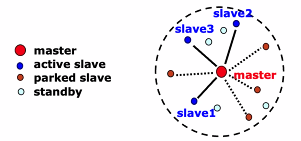
\includegraphics[width=0.8\textwidth]{Pictures/Pasted image 20251021084008.png}
\end{figure}}
\#\#\# Frame The \textbf{frame structure} includes: - \textbf{Access
code}: Synchronization and piconet ID.\\
- \textbf{Header}: Contains an 18-bit pattern repeated three times with
information such as address (3 bits for 7 destinations), message type,
flow control (F), acknowledgment (A), sequence number (S), and header
error correction (HEC).\\
- \textbf{Payload}: Carries data, ranging from 0--2740 bits.
\pandocbounded{\begin{figure}[h]
\centering
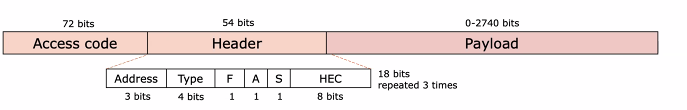
\includegraphics[width=0.8\textwidth]{Pictures/Pasted image 20251021084404.png}
\end{figure}}

\begin{longtable}[]{@{}
  >{\raggedright\arraybackslash}p{(\linewidth - 0\tabcolsep) * \real{0.0556}}@{}}
\toprule\noalign{}
\begin{minipage}[b]{\linewidth}\raggedright
\#\#\# Layers Bluetooth communication follows a layered architecture: -
The \textbf{PHY layer} deals with the physical transmission of data. -
The \textbf{MAC layer} handles access control and defines data packet
formats.
\end{minipage} \\
\midrule\noalign{}
\endhead
\bottomrule\noalign{}
\endlastfoot
\#\#\# Radio Layer - Bluetooth operates in the \textbf{2.4 GHz ISM
band}, divided into \textbf{79 channels of 1 MHz each}. - Uses
\textbf{GFSK modulation} (Gaussian Frequency Shift Keying) at 1 Mbit/s.
- Frequency-Hopping Spread Spectrum (FHSS) is used, with \textbf{1600
hops per second}, each frequency being used for only \textbf{625 µs} to
avoid interference.
\pandocbounded{\begin{figure}[h]
\centering
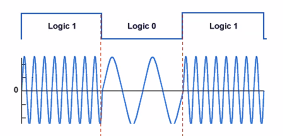
\includegraphics[width=0.8\textwidth]{Pictures/Pasted image 20251021084939.png}
\end{figure}}
\pandocbounded{\begin{figure}[h]
\centering
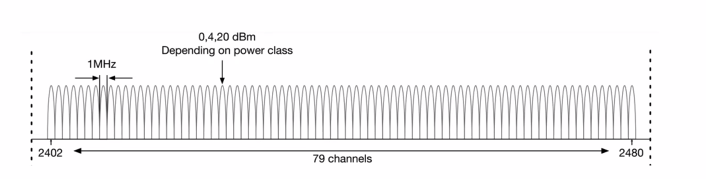
\includegraphics[width=0.8\textwidth]{Pictures/Pasted image 20251021085628.png}
\end{figure}} \\
\end{longtable}

\subsection{FHSS Coordination}\label{fhss-coordination}

\begin{itemize}
\tightlist
\item
  Bluetooth devices must \textbf{synchronize} their frequency hopping
  sequences during \textbf{link establishment}.\\
\item
  \textbf{Frequency hopping} helps reduce interference, ensuring smooth
  communication between devices.
\end{itemize}

\subsection{Baseband Layer}\label{baseband-layer}

\begin{itemize}
\tightlist
\item
  The \textbf{Baseband layer} is responsible for organizing the
  communication between devices, similar to the \textbf{MAC layer} in
  LANs.\\
\item
  Bluetooth uses \textbf{Time Division Duplex (TDD)} with 625 µs
  slots.\\
\item
  Communication alternates between the \textbf{Master} (even slots) and
  \textbf{Slave} (odd slots), with different frequency channels used in
  each slot.
  \pandocbounded{\begin{figure}[h]
\centering
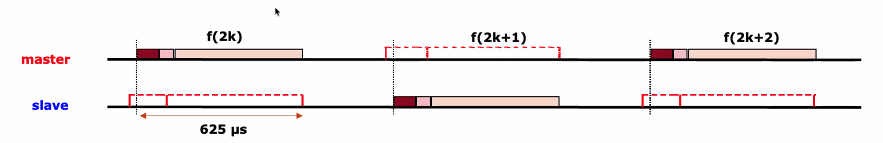
\includegraphics[width=0.8\textwidth]{Pictures/Pasted image 20251021090022.png}
\end{figure}}
\end{itemize}

\begin{longtable}[]{@{}
  >{\raggedright\arraybackslash}p{(\linewidth - 0\tabcolsep) * \real{0.0556}}@{}}
\toprule\noalign{}
\endhead
\bottomrule\noalign{}
\endlastfoot
\#\#\# Connection Procedure 1. \textbf{Inquiry Phase:} - Master
initializes communication and establishes the hopping sequence for the
piconet. - Devices go into sleep mode. 2. \textbf{Paging Phase:} -
Master pages a Slave, who responds with a \textbf{Device Access Code
(DAC)}. - Master sends the list of frequency hops to the Slave, and the
Slave replies with a second DAC. \\
Collision between two slaves is very rare to happen. If it does, he
simply ask for a retrasmission. Odd and even distinction is done because
master cannot trasmit and receive at the same time. \\
\end{longtable}

\subsection{L2CAP}\label{l2cap}

\begin{itemize}
\tightlist
\item
  The \textbf{Logical Link Control and Adaptation Protocol (L2CAP)}
  handles \textbf{multiplexing}, \textbf{segmentation},
  \textbf{reassembly}, \textbf{QoS} (Quality of Service), and
  \textbf{group management}.\\
\item
  Two types of communication:

  \begin{itemize}
  \tightlist
  \item
    \textbf{Synchronous Connection-Oriented (SCO)}: Low-latency,
    connection-oriented service.\\
  \item
    \textbf{Asynchronous Connection-Less (ACL)}: Packet-oriented,
    error-checked, and asynchronous.
  \item
    If a payload encapsulated in the frame is corrupted, it is
    retransmitted.
  \end{itemize}
\end{itemize}

\section{BR/EDR}\label{bredr-1}

\subsection{L2CAP ACL Example}\label{l2cap-acl-example}

\begin{itemize}
\tightlist
\item
  \textbf{L2CAP ACL} packets can be 1, 3, or 5 slots long, with each
  slot occupying a different frequency channel.\\
\item
  This reduces overhead by minimizing the need for extra headers and
  guard times, making data transmission more efficient.
  \pandocbounded{\begin{figure}[h]
\centering
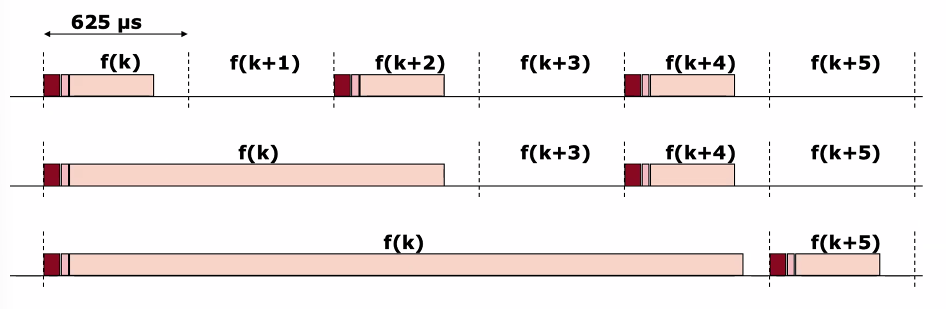
\includegraphics[width=0.8\textwidth]{Pictures/Pasted image 20251021091451.png}
\end{figure}}
\end{itemize}

\subsection{LMP (Link Manager
Protocol)}\label{lmp-link-manager-protocol}

\begin{itemize}
\tightlist
\item
  The \textbf{Link Manager Protocol (LMP)} is responsible for
  \textbf{setting up and managing Baseband connections}.\\
\item
  LMP handles authentication, link configuration, and \textbf{power
  management}.\\
\item
  It exchanges \textbf{Protocol Data Units (PDUs)} between two paired
  devices to configure settings such as pairing, authentication, and
  packet size optimization.
\end{itemize}

\begin{longtable}[]{@{}
  >{\raggedright\arraybackslash}p{(\linewidth - 0\tabcolsep) * \real{0.0556}}@{}}
\toprule\noalign{}
\begin{minipage}[b]{\linewidth}\raggedright
\#\#\# HCI (Host Controller Interface) - The \textbf{Host Controller
Interface (HCI)} provides a command interface between the \textbf{Host}
(upper layers) and \textbf{Controller} (Baseband, LMP, PHY). - It allows
the protocol stack to be split between two hardware pieces, connected
through a \textbf{Host Controller Transport} layer (UART, RS232, or
USB).
\end{minipage} \\
\midrule\noalign{}
\endhead
\bottomrule\noalign{}
\endlastfoot
\#\#\# Profiles - \textbf{Profiles} define application-specific protocol
stacks in Bluetooth. - There are nearly \textbf{40 profiles}, each
supporting different applications, ranging from narrow uses (e.g.,
headset profile) to more flexible ones (e.g., \textbf{PAN} -- Personal
Area Network). - Networking capabilities depend on the selected
profile. \\
\end{longtable}

\section{BLE}\label{ble}

\subsection{Overview}\label{overview-1}

\begin{itemize}
\tightlist
\item
  \textbf{Bluetooth Low Energy (BLE)} is a more recent extension of
  Bluetooth, designed specifically for \textbf{low-power IoT devices}
  and sensors.\\
\item
  Key differences from BR/EDR:

  \begin{itemize}
  \tightlist
  \item
    \textbf{Fewer channels}: 40 (2 MHz) vs.~79 (1 MHz).
  \item
    Uses \textbf{GFSK modulation} only.\\
  \item
    Data rate of up to \textbf{2 Mbit/s}, which results in
    \textbf{shorter transmission times} and \textbf{lower energy
    consumption}.\\
  \item
    \textbf{Adaptive frequency hopping}, with potentially fewer hops.\\
  \item
    New error protection codes for more reliable communication.
  \end{itemize}
\end{itemize}

\begin{center}\rule{0.5\linewidth}{0.5pt}\end{center}

\section{BLE}\label{ble-1}

\subsection{Communication Modes}\label{communication-modes}

\begin{itemize}
\tightlist
\item
  BLE nodes can take on \textbf{4 roles}, as opposed to just \textbf{2
  in BR/EDR}:

  \begin{itemize}
  \tightlist
  \item
    \textbf{Broadcaster}: Sends advertisements but does not accept
    connections (e.g., iBeacon).
  \item
    \textbf{Observer}: Listens for advertisements but does not initiate
    connections.
  \item
    \textbf{Peripheral}: Sends advertisements and may accept
    connections, acting as a \textbf{Slave}.
  \item
    \textbf{Central}: Can initiate connections and acts as the
    \textbf{Master} after receiving information about a peripheral.
  \end{itemize}
\end{itemize}

\begin{center}\rule{0.5\linewidth}{0.5pt}\end{center}

\section{BLE}\label{ble-2}

\subsection{New Profiles}\label{new-profiles}

\begin{itemize}
\tightlist
\item
  \textbf{New BLE profiles} support specialized applications, such as:

  \begin{itemize}
  \tightlist
  \item
    \textbf{Heart Rate Profile}, \textbf{Internet Protocol Support
    Profile}, and the \textbf{Mesh Profile}.
  \end{itemize}
\item
  \textbf{Mesh Profile} enables \textbf{multi-hop communication} in
  \textbf{mesh networks}:

  \begin{itemize}
  \tightlist
  \item
    \textbf{Relay nodes} forward messages between devices.\\
  \item
    \textbf{Low Power Nodes (LPN)} sleep and wake periodically to
    exchange data with \textbf{Friend Nodes}, which store messages while
    the LPN is asleep.
  \item
    \textbf{Managed flooding} prevents loops in the network.
    \pandocbounded{\begin{figure}[h]
\centering
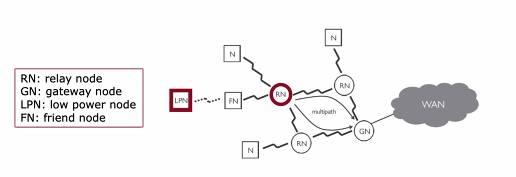
\includegraphics[width=0.8\textwidth]{Pictures/Pasted image 20251021092446.png}
\end{figure}}
  \end{itemize}
\end{itemize}

\begin{longtable}[]{@{}
  >{\raggedright\arraybackslash}p{(\linewidth - 0\tabcolsep) * \real{0.0556}}@{}}
\toprule\noalign{}
\endhead
\bottomrule\noalign{}
\endlastfoot
\#\# BR/EDR vs.~BLE \#\#\# Comparison The following table compares the
features of \textbf{BR/EDR} and \textbf{BLE}: \\
\textbar{} Feature \textbar{} \textbf{BR/EDR} \textbar{} \textbf{BLE}
\textbar{} \textbar{} --------------------- \textbar{}
------------------------- \textbar{} -------------------------------
\textbar{} \textbar{} \textbf{Power consumption} \textbar{} Higher
\textbar{} Lower \textbar{} \textbar{} \textbf{Data rate} \textbar{} Up
to \textbf{3 Mbps} (8-DPSK) \textbar{} Up to \textbf{2 Mbps} (GFSK)
\textbar{} \textbar{} \textbf{Latency} \textbar{} Lower \textbar{}
Higher \textbar{} \textbar{} \textbf{Connection type} \textbar{}
Point-to-point \textbar{} Point-to-point, broadcast, mesh \textbar{}
\textbar{} \textbf{Use cases} \textbar{} Audio, peripherals \textbar{}
IoT, wearables, sensors \textbar{} \textbar{} \textbf{Compatibility}
\textbar{} Classic Bluetooth devices \textbar{} Bluetooth 4.0+
\textbar{} \\
\#\#\# Key Differences - \textbf{BR/EDR} is ideal for applications
requiring high data rates and low latency, such as audio and video
streaming, while \textbf{BLE} is optimized for low-power devices such as
wearables, sensors, and IoT devices. \\
\end{longtable}


% --- Chapter from 06. IEEE 802.15.4 technologies.md ---
\subsection{General description}\label{general-description}

\subsubsection{Overview}\label{overview}

\begin{itemize}
\tightlist
\item
  \textbf{IEEE 800.15.4} defines the \textbf{Physical (PHY)} and
  \textbf{Media Access Control (MAC)} sublayers for Low-Rate Wireless
  Personal Area Networks (LR-WPANs).
\item
  It is designed for easy installation, reliability, extremely low cost,
  reasonable battery life, and relaxed throughput.
\item
  It supports a large number of nodes (unlike BLE) and asynchronous
  communication of small data packets.
\item
  It is the foundation used by protocols like \textbf{ZigBee} and
  \textbf{6LoWPAN}.
\end{itemize}

\subsubsection{Operational frequency}\label{operational-frequency}

\begin{longtable}[]{@{}llll@{}}
\toprule\noalign{}
Band & 868.3 MHz & 915 MHz & 2.4 GHz \\
\midrule\noalign{}
\endhead
\bottomrule\noalign{}
\endlastfoot
\textbf{Channels} & 1 & 10 & 16 \\
\textbf{Bandwidth/channel} & 600 KHz & 2 MHz & 2 MHz \\
\textbf{Modulation} & BPSK & BPSK & QPSK \\
\textbf{Bitrate} & \textasciitilde20 Kbit/s & \textasciitilde40 Kbit/s &
\textasciitilde250 Kbit/s \\
\textbf{Sensitivity} & & -92 dBm & -85 dBm \\
\textbf{Transmission power} & & \textless1 mW (low-power) & \\
\textbf{Availability} & Europe & America & Worldwide \\
\textbf{Range} & & 10-75 m (typically 30 m) & \\
\textbf{Interference} & & Few & Severe (very crowded) \\
\end{longtable}

\subsubsection{Types of nodes}\label{types-of-nodes}

\begin{itemize}
\tightlist
\item
  \textbf{Full Function Device (FFD):}

  \begin{itemize}
  \tightlist
  \item
    Has full PHY and MAC capabilities.
  \item
    Can relay messages.
  \item
    Can act as a PAN coordinator.
  \item
    Supports any topology.
  \end{itemize}
\item
  \textbf{Reduced Function Device (RFD):}

  \begin{itemize}
  \tightlist
  \item
    Simpler implementation with reduced functions.
  \item
    Can only talk to an FFD and cannot be a PAN coordinator.
  \item
    Cannot relay data (acts only as an end node).
  \item
    Limited to star topology.
  \end{itemize}
\end{itemize}

\subsubsection{Topologies}\label{topologies}

\begin{itemize}
\tightlist
\item
  Star topology
\item
  Mesh topology
\item
  Cluster tree topology more masters than BLE
\end{itemize}

\pandocbounded{\begin{figure}[h]
\centering
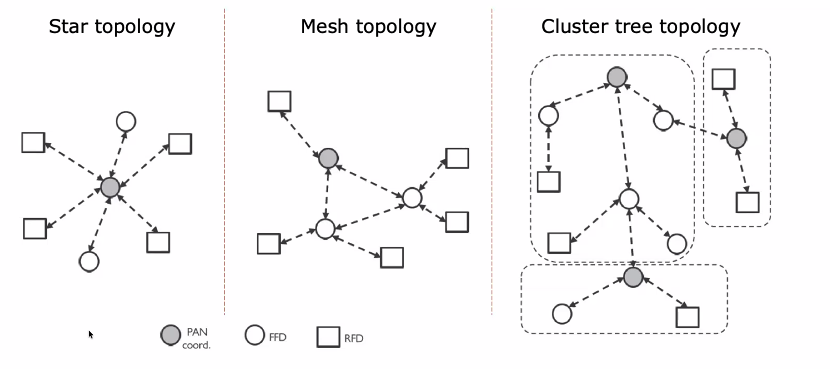
\includegraphics[width=0.8\textwidth]{Pictures/Pasted image 20251021094151.png}
\end{figure}}

\subsubsection{Frame structure}\label{frame-structure}

\begin{itemize}
\tightlist
\item
  \textbf{Preamble (32 bits):} For synchronization.
\item
  \textbf{Start of Packet Delimiter (8 bits)}.
\item
  \textbf{PHY Header (8 bits):} Indicates PSDU length.
\item
  \textbf{PSDU (0 to 1016 bits / 0-127 bytes):} The data field.
  \pandocbounded{\begin{figure}[h]
\centering
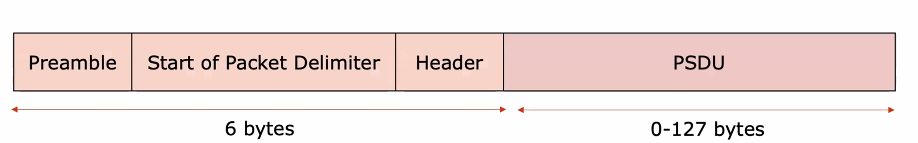
\includegraphics[width=0.8\textwidth]{Pictures/Pasted image 20251021094257.png}
\end{figure}}
\end{itemize}

\subsubsection{MAC layer}\label{mac-layer}

\pandocbounded{\begin{figure}[h]
\centering
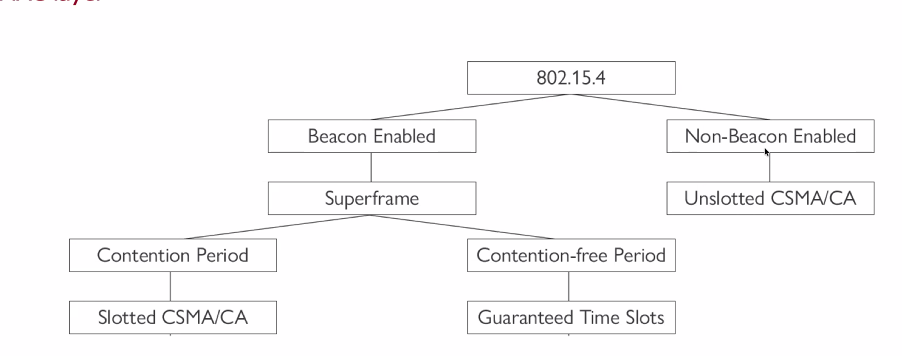
\includegraphics[width=0.8\textwidth]{Pictures/Pasted image 20251021094457.png}
\end{figure}}
The MAC layer operates in two main modes:

\begin{itemize}
\tightlist
\item
  \textbf{Beacon-enabled mode:}

  \begin{itemize}
  \tightlist
  \item
    The PAN coordinator periodically sends \textbf{beacons} for
    synchronization.
  \item
    Time is divided into \textbf{Superframes} (the active part).
  \item
    The Superframe is divided into 16 time slots and has two parts:

    \begin{enumerate}
    \def\labelenumi{\arabic{enumi}.}
    \tightlist
    \item
      \textbf{Contention Access Period (CAP):} Uses slotted CSMA/CA for
      channel access.
    \item
      \textbf{Contention Free Protocol (CFP) (optional):} Uses
      \textbf{Guaranteed Time Slots (GTS)} allocated by the coordinator
      for dedicated, contention-free resources.
      \pandocbounded{\begin{figure}[h]
\centering
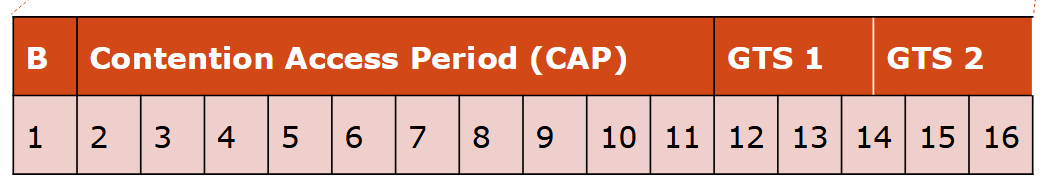
\includegraphics[width=0.8\textwidth]{Pictures/Pasted image 20251021095218.png}
\end{figure}}
    \end{enumerate}
  \item
    An \textbf{Inactive part} allows nodes to sleep to save power.
  \item
    The ratio of superframe duration to beacon interval is the
    \textbf{duty cycle}.
  \end{itemize}
\item
  \textbf{Non-beacon-enabled mode:}

  \begin{itemize}
  \tightlist
  \item
    No periodic beacons are sent.
  \item
    Channel access uses \textbf{unslotted CSMA/CA}.
  \item
    Synchronization is not required, which saves power from beacon
    listening.
  \item
    Devices must use \textbf{active scanning} (sending a Beacon Request)
    to join the network.
  \end{itemize}
\end{itemize}

\subsubsection{Security}\label{security}

The MAC layer provides several security services: * \textbf{Unsecured:}
No security. * \textbf{Access Control List (ACL):} Accepts/rejects
frames based on the source node. * \textbf{Secured:} Implements multiple
mechanisms: * Access control. * Data confidentiality (symmetric
encryption). * Frame integrity. * Sequential freshness protection
(prevents frame replay).

\subsubsection{Amendments}\label{amendments}

\begin{itemize}
\tightlist
\item
  \textbf{Timeslotted Channel Hopping (TSCH):} Designed for industrial
  processes. It works in non-beacon mode and uses channel hopping to
  improve reliability.
\item
  \textbf{Deterministic and Synchronous Multi-channel Extension (DSME):}
  Implements the use of multiple channels within the same superframe for
  robustness.
\end{itemize}

\begin{center}\rule{0.5\linewidth}{0.5pt}\end{center}

\subsection{ZigBee}\label{zigbee}

\subsubsection{Overview}\label{overview-1}

\begin{itemize}
\tightlist
\item
  An industrial standard for IoT promoted by the Zigbee Alliance.
\item
  It is built on top of the IEEE 800.15.4 PHY and MAC layers.
\item
  It defines the \textbf{Network (NWK)}, \textbf{Application Support
  (APS)}, and \textbf{Application Layers (AF)}.
  \pandocbounded{\begin{figure}[h]
\centering
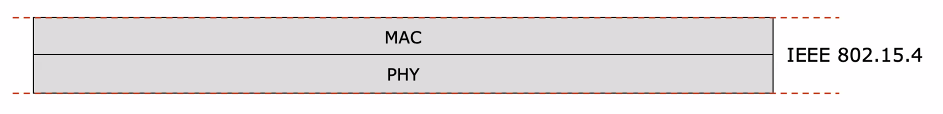
\includegraphics[width=0.8\textwidth]{Pictures/Pasted image 20251021100429.png}
\end{figure}}
\end{itemize}

\subsubsection{Applications}\label{applications}

\begin{itemize}
\tightlist
\item
  Building automation (HVAC, lighting, metering)
\item
  Personal healthcare (patient monitoring)
\item
  Industrial automation (asset management, process control)
\item
  Consumer electronics (remotes)
\item
  PC peripherals (mouse, keyboard)
\end{itemize}

\subsubsection{Network layer:
functionalities}\label{network-layer-functionalities}

\begin{itemize}
\tightlist
\item
  Starting, joining, and leaving a network.
\item
  Configuring new devices.
\item
  Assigning addresses to devices.
\item
  Routing and route discovery.
\item
  Applying and removing security to frames.
\end{itemize}

\subsubsection{Network layer: topology}\label{network-layer-topology}

\begin{itemize}
\item
  \textbf{Star Network:} A central coordinator (FDD) communicates with
  end devices (FDD or RFD).
  \pandocbounded{\begin{figure}[h]
\centering
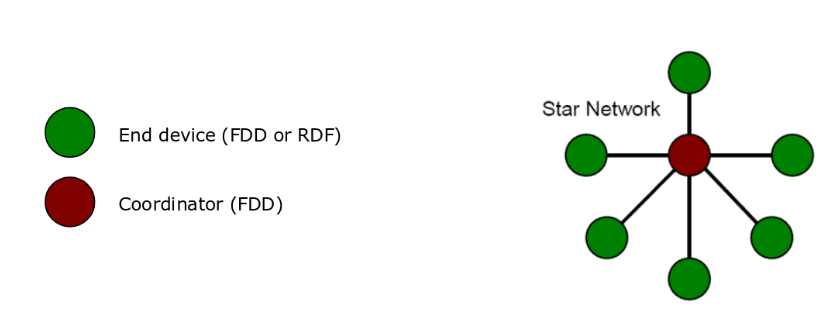
\includegraphics[width=0.8\textwidth]{Pictures/Pasted image 20251022084550.png}
\end{figure}}
\item
  \textbf{Mesh Network:} The network is extended using \textbf{ZigBee
  routers (FDDs)} that relay data, allowing nodes to communicate beyond
  the coordinator's direct range.
  \pandocbounded{\begin{figure}[h]
\centering
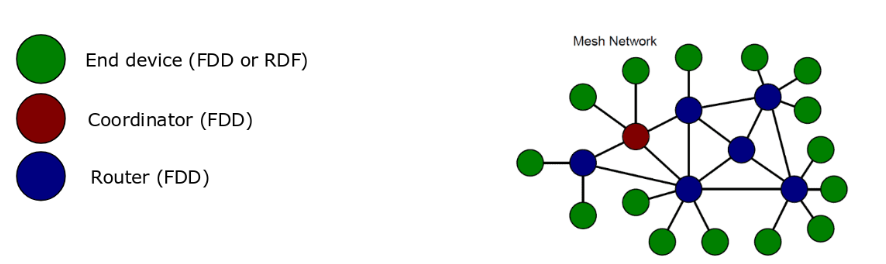
\includegraphics[width=0.8\textwidth]{Pictures/Pasted image 20251022084615.png}
\end{figure}}
  \#\#\#\# Network layer: addressing Each device has two identifiers:
\end{itemize}

\begin{enumerate}
\def\labelenumi{\arabic{enumi}.}
\tightlist
\item
  \textbf{Extended Address (64-bit):} A unique, universal IEEE address
  assigned during production (like a MAC address).
\item
  \textbf{Short Address (16-bit):} A dynamic ID assigned by the PAN
  Coordinator when a device joins the network (like an IP address). This
  allows for up to \textasciitilde65,000 nodes.
\end{enumerate}

\subsubsection{Network layer: routing}\label{network-layer-routing}

\begin{itemize}
\tightlist
\item
  Can be \textbf{hierarchical} (following the network tree).
\item
  Also uses \textbf{dynamic ``best'' path} searching based on the
  \textbf{AODV (Ad-hoc On-demand Distance Vector)} protocol.
\item
  Routers are discovered on-demand.
\item
  The algorithm finds the minimal cost path, calculated from the
  probability of packet delivery on each link. \[
  C\{l\} = min(7,[\frac{1}{p_l^4}])
  \] where \(p_l\) is the probability of a packet delivery on link
  \(l\). It depends on the quality of the link.
\end{itemize}

\subsubsection{Application layer:
overview}\label{application-layer-overview}

Consists of three sublayers: 1. \textbf{Application Support (APS)} 2.
\textbf{ZigBee Device Objects (ZDO)} 3. \textbf{Application Framework
(AF)} (manufacturer-defined apps)
\pandocbounded{\begin{figure}[h]
\centering
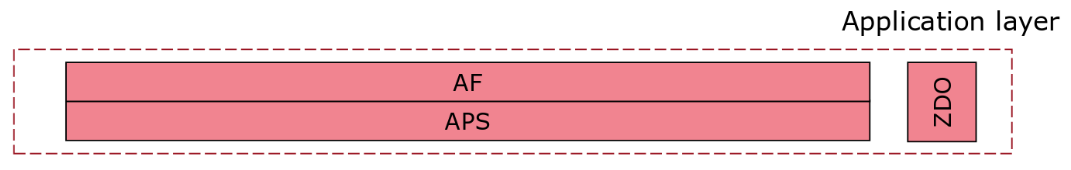
\includegraphics[width=0.8\textwidth]{Pictures/Pasted image 20251022084949.png}
\end{figure}}

\subsubsection{Application layer: APS}\label{application-layer-aps}

Provides services such as: * \textbf{Address mapping} (between 64-bit
and 16-bit addresses). * \textbf{Fragmentation and reassembly}. *
\textbf{Security} (encryption/decryption). * \textbf{Binding} (matching
two devices based on their services). * \textbf{Service Discovery}. *
\textbf{Group Addressing} (e.g., ``turn on all lights'').

\subsubsection{Application layer: ZDO}\label{application-layer-zdo}

A special application that handles key network functions: * Defining the
device's role (Coordinator, Router, End Device). * Device discovery and
network formation. * Network management (joining/leaving). * Security
management (key distribution). * Network address management (resolving
conflicts).

\subsubsection{Application layer: AF}\label{application-layer-af}

\begin{itemize}
\tightlist
\item
  Provides the platform for running the actual user application
  (Application Objects).
\item
  Provides application \textbf{profiles} to ensure interoperability
  between different manufacturers.
\item
  Exposes ZDO functions to the applications.
\end{itemize}

\begin{center}\rule{0.5\linewidth}{0.5pt}\end{center}

\subsection{6LowPAN}\label{lowpan}

\subsubsection{Overview}\label{overview-2}

\begin{itemize}
\tightlist
\item
  \textbf{6LoWPAN} is an IETF standard for \textbf{IPv6 over Low-Rate
  Wireless Personal Area Networks} (i.e., IEEE 800.15.4).
\item
  The goal is to transform any device into an IPv6-addressable host.
\item
  It introduces a \textbf{6LowPAN Adaptation layer} between the IPv6
  Network layer and the 800.15.4 MAC layer.
\end{itemize}

\subsubsection{IPv6}\label{ipv6}

\begin{itemize}
\tightlist
\item
  \textbf{Problem:} IPv4 has up to 4B addresses.
\item
  We may need in the future a larger address space.
\item
  How to solve?

  \begin{itemize}
  \tightlist
  \item
    Classless addressing
  \item
    Private addressing and NAT.
  \item
    \textbf{IPv6}
  \end{itemize}
\item
  IPv6 addresses are written in \textbf{hexadecimal} separated by ``:''.
\item
  Three types: \textbf{Unicast}, \textbf{Multicast}, \textbf{Anycast},
  Broadcast \textbf{not} supported.
\item
  It can have multiple addresses: \textbf{Link-Local, Unique-Local,
  Global}
\end{itemize}

\paragraph{Link-Local Address}\label{link-local-address}

\begin{itemize}
\tightlist
\item
  \textbf{Prefix:} Starts with \texttt{FE80::/10} (the first 10 bits are
  equal to \texttt{1111\ 1110\ 10}).
\item
  \textbf{Purpose:} Can be used to reach nodes attached to the same link
  without a globally unique address. If several IPv6-enabled nodes
  connect to a switch, they will \textbf{auto-configure} their
  interfaces with link-local addresses, discover each other, and be able
  to communicate.
\item
  \textbf{Key Features:}

  \begin{itemize}
  \tightlist
  \item
    Contains the MAC address of the node in the EUI-64 format.
  \item
    \textbf{Not routable:} IPv6 routers must not forward packets having
    link-local source/destination address.
  \item
    All IPv6-enabled interfaces have a link-local unicast address.
  \end{itemize}
\item
  \textbf{Structure:} 10 bits for the prefix, 54 reserved bits (zeros),
  and 64 bits for the Interface ID.
\end{itemize}

\pandocbounded{\begin{figure}[h]
\centering
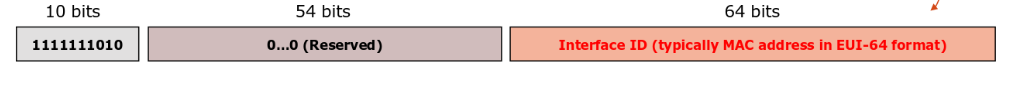
\includegraphics[width=0.8\textwidth]{Pictures/Pasted image 20251022091212.png}
\end{figure}}

\begin{center}\rule{0.5\linewidth}{0.5pt}\end{center}

\paragraph{Unique Local Address (ULA)}\label{unique-local-address-ula}

\begin{itemize}
\tightlist
\item
  \textbf{Prefix:} Starts with a prefix \texttt{FC00::/7} (the first 7
  bits are equal to \texttt{1111\ 110}).
\item
  \textbf{Purpose:} It is a \textbf{private} IPv6 address used for
  internal communication within an organization or network, similar to
  private IPv4 addresses.
\item
  \textbf{Key Features:}

  \begin{itemize}
  \tightlist
  \item
    \textbf{Not routable} to the public Internet; won't overlap with any
    other ISP-assigned range.
  \item
    It allows sites to be interconnected without creating any address
    conflicts.
  \item
    It supports flexible \textbf{subnetting} and routing internally
    within the private network.
  \end{itemize}
\item
  \textbf{Structure:} 7 bits for the prefix, 1 bit for `L', 40 bits for
  the Global Routing Prefix (randomly generated number ensuring global
  uniqueness), 16 bits for the Subnet ID, and 64 bits for the Interface
  ID (typically the MAC address in EUI-64 format).
  \pandocbounded{\begin{figure}[h]
\centering
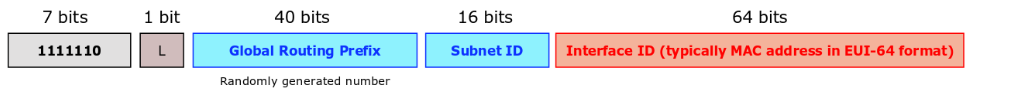
\includegraphics[width=0.8\textwidth]{Pictures/Pasted image 20251022091229.png}
\end{figure}}
\end{itemize}

\begin{center}\rule{0.5\linewidth}{0.5pt}\end{center}

\paragraph{Global Unicast Address}\label{global-unicast-address}

\begin{itemize}
\tightlist
\item
  \textbf{Prefix:} Starts with a prefix \texttt{2000::/3} (the first 3
  bits are equal to \texttt{100}).
\item
  \textbf{Purpose:} \textbf{Public address:} it can be used to route IP
  datagrams over the Internet.
\item
  \textbf{Key Features:}

  \begin{itemize}
  \tightlist
  \item
    The structure consists of a 48-bit prefix and a 16-bit subnet ID
    also referred to as \textbf{Site-Level Aggregator (SLA)}.
  \item
    The prefix is variable, defined from router advertisements, and some
    IP addresses can be reserved.
  \end{itemize}
\item
  \textbf{Structure:} 3 bits for the prefix, 45 bits for the Global
  Routing Prefix, 16 bits for the Subnet ID, and 64 bits for the
  Interface ID.

  \begin{itemize}
  \tightlist
  \item
    The first 64 bits make up the \textbf{Network ID (NetID) Prefix}.
  \item
    The last 64 bits make up the \textbf{HostID Suffix}.
  \end{itemize}
\end{itemize}

\pandocbounded{\begin{figure}[h]
\centering
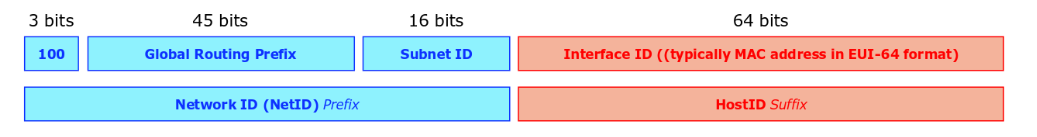
\includegraphics[width=0.8\textwidth]{Pictures/Pasted image 20251022091245.png}
\end{figure}}

\subsubsection{IPv6 assignment}\label{ipv6-assignment}

\begin{enumerate}
\def\labelenumi{\arabic{enumi}.}
\tightlist
\item
  Manual config
\item
  Stateful config with \textbf{DHCPv6} protocol
\item
  Stateless autoconfig without DHCP, IPv6 nodes can connect to a network
  and automatically generate a Global IPv6 address with no dedicated
  server. \#\#\#\# Digression: IPv6 for IoT
\end{enumerate}

\begin{itemize}
\tightlist
\item
  \textbf{Benefits} of using IPv6 protocols in IoT scenarios:

  \begin{itemize}
  \tightlist
  \item
    Can connect potentially infinite number of IoT.
  \item
    Easily connect to other devices without the need of translation.
  \item
    Address/manage/access any IoT device from the Internet (no
    saturation).
  \item
    Use well-known socket API for the deployment of the network
    applications.
  \item
    Easily re-use tools for managing, commissioning, and diagnosing
    IP-based networks.
  \end{itemize}
\item
  \textbf{Problem:} There is a large mismatch between IPv6 and IEEE
  800.15.4.

  \begin{itemize}
  \tightlist
  \item
    \textbf{MTU Size:} The minimum IPv6 MTU is \textbf{1280 bytes}.
  \item
    \textbf{800.15.4 MTU:} The maximum 800.15.4 frame payload is
    \textbf{127 bytes}.
  \item
    \textbf{Header Overhead:} The standard IPv6 header is \textbf{40
    bytes}, which would consume nearly one-third of the entire 800.15.4
    payload.
  \end{itemize}
\end{itemize}

\begin{center}\rule{0.5\linewidth}{0.5pt}\end{center}

\subsubsection{General architecture}\label{general-architecture}

\begin{itemize}
\tightlist
\item
  6LoWPAN networks connect to the internet using standard \textbf{IPv6
  edge routers}.
\item
  This avoids the need for special application-layer gateways (like
  those used in ZigBee).
\item
  Network nodes can be \textbf{Hosts (H)} (end devices) or
  \textbf{Routers (R)} (FFDs).
  \pandocbounded{\begin{figure}[h]
\centering
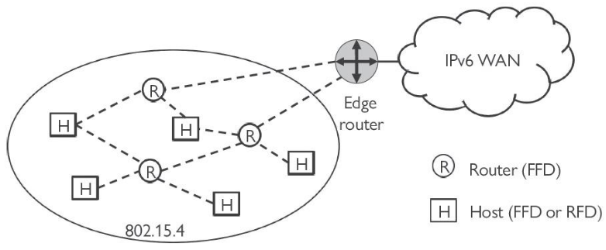
\includegraphics[width=0.8\textwidth]{Pictures/Pasted image 20251022095130.png}
\end{figure}}
  \#\#\#\# Addressing To solve the MTU and overhead problem, 6LoWPAN
  uses:
\end{itemize}

\begin{enumerate}
\def\labelenumi{\arabic{enumi}.}
\tightlist
\item
  \textbf{Header compression}
\item
  \textbf{Fragmentation}
\end{enumerate}

\subsubsection{Header compression}\label{header-compression}

\begin{itemize}
\tightlist
\item
  Works by eliding or compressing redundant information from the 40-byte
  IPv6 header.
\item
  Fields like Version (always 6), Payload Length (derived from data-link
  layer), and Traffic Class/Flow Label (often zero) can be compressed or
  removed. \#\#\#\#\# HC1 format:
\end{itemize}

\begin{longtable}[]{@{}
  >{\raggedright\arraybackslash}p{(\linewidth - 14\tabcolsep) * \real{0.2542}}
  >{\raggedright\arraybackslash}p{(\linewidth - 14\tabcolsep) * \real{0.0847}}
  >{\raggedright\arraybackslash}p{(\linewidth - 14\tabcolsep) * \real{0.0847}}
  >{\raggedright\arraybackslash}p{(\linewidth - 14\tabcolsep) * \real{0.0847}}
  >{\raggedright\arraybackslash}p{(\linewidth - 14\tabcolsep) * \real{0.0847}}
  >{\raggedright\arraybackslash}p{(\linewidth - 14\tabcolsep) * \real{0.0847}}
  >{\raggedright\arraybackslash}p{(\linewidth - 14\tabcolsep) * \real{0.2034}}
  >{\raggedright\arraybackslash}p{(\linewidth - 14\tabcolsep) * \real{0.1186}}@{}}
\toprule\noalign{}
\begin{minipage}[b]{\linewidth}\raggedright
7 bit
\end{minipage} & \begin{minipage}[b]{\linewidth}\raggedright
1 bit
\end{minipage} & \begin{minipage}[b]{\linewidth}\raggedright
2 bit
\end{minipage} & \begin{minipage}[b]{\linewidth}\raggedright
2 bit
\end{minipage} & \begin{minipage}[b]{\linewidth}\raggedright
2 bit
\end{minipage} & \begin{minipage}[b]{\linewidth}\raggedright
1 bit
\end{minipage} & \begin{minipage}[b]{\linewidth}\raggedright
8 bit
\end{minipage} & \begin{minipage}[b]{\linewidth}\raggedright
\end{minipage} \\
\midrule\noalign{}
\endhead
\bottomrule\noalign{}
\endlastfoot
HC101000010 & TF & SA & DA & NH & HC2 & HopLimit & Payload \\
\end{longtable}

\paragraph{IPHC format}\label{iphc-format}

A more efficient format that uses context-based compression.

\begin{longtable}[]{@{}
  >{\raggedright\arraybackslash}p{(\linewidth - 20\tabcolsep) * \real{0.1507}}
  >{\raggedright\arraybackslash}p{(\linewidth - 20\tabcolsep) * \real{0.0685}}
  >{\raggedright\arraybackslash}p{(\linewidth - 20\tabcolsep) * \real{0.0685}}
  >{\raggedright\arraybackslash}p{(\linewidth - 20\tabcolsep) * \real{0.0685}}
  >{\raggedright\arraybackslash}p{(\linewidth - 20\tabcolsep) * \real{0.0685}}
  >{\raggedright\arraybackslash}p{(\linewidth - 20\tabcolsep) * \real{0.1370}}
  >{\raggedright\arraybackslash}p{(\linewidth - 20\tabcolsep) * \real{0.0685}}
  >{\raggedright\arraybackslash}p{(\linewidth - 20\tabcolsep) * \real{0.0685}}
  >{\raggedright\arraybackslash}p{(\linewidth - 20\tabcolsep) * \real{0.1370}}
  >{\raggedright\arraybackslash}p{(\linewidth - 20\tabcolsep) * \real{0.0685}}
  >{\raggedright\arraybackslash}p{(\linewidth - 20\tabcolsep) * \real{0.0959}}@{}}
\toprule\noalign{}
\begin{minipage}[b]{\linewidth}\raggedright
3 bit
\end{minipage} & \begin{minipage}[b]{\linewidth}\raggedright
2 bit
\end{minipage} & \begin{minipage}[b]{\linewidth}\raggedright
1 bit
\end{minipage} & \begin{minipage}[b]{\linewidth}\raggedright
2 bit
\end{minipage} & \begin{minipage}[b]{\linewidth}\raggedright
1 bit
\end{minipage} & \begin{minipage}[b]{\linewidth}\raggedright
1 bit
\end{minipage} & \begin{minipage}[b]{\linewidth}\raggedright
2 bit
\end{minipage} & \begin{minipage}[b]{\linewidth}\raggedright
1 bit
\end{minipage} & \begin{minipage}[b]{\linewidth}\raggedright
1 bit
\end{minipage} & \begin{minipage}[b]{\linewidth}\raggedright
2 bit
\end{minipage} & \begin{minipage}[b]{\linewidth}\raggedright
\end{minipage} \\
\midrule\noalign{}
\endhead
\bottomrule\noalign{}
\endlastfoot
IPHC011 & TF & NH & HLIM & CID & SAC(S) & SAM & M & DAC(D) & DAM &
Payload \\
\end{longtable}

\begin{longtable}[]{@{}lll@{}}
\toprule\noalign{}
SAM/DAM value & Inline & IID \\
\midrule\noalign{}
\endhead
\bottomrule\noalign{}
\endlastfoot
000 & 128 & address fully inline \\
001 & 64 & link-local 64-bit Interface ID \\
010 & 16 & link-local 16-bit short address \\
011 & 0 & link-local + link-layer source address \\
100 & & reserved \\
101 & 64 & context + 64-bit Interface ID \\
110 & 16 & context + 16-bit short address \\
111 & 0 & context \\
\end{longtable}

\subsubsection{Fragmentation}\label{fragmentation}

\begin{itemize}
\tightlist
\item
  If a packet is still too large after compression, it must be
  fragmented.
\item
  Fragmentation information is carried in a \textbf{Fragment Header}.
\end{itemize}

\paragraph{First Fragment}\label{first-fragment}

\begin{longtable}[]{@{}lll@{}}
\toprule\noalign{}
8 bit & 11 bit & 16 bit \\
\midrule\noalign{}
\endhead
\bottomrule\noalign{}
\endlastfoot
11000xxx & Size & Tag \\
\end{longtable}

\paragraph{Subsequent Fragments}\label{subsequent-fragments}

\begin{longtable}[]{@{}llll@{}}
\toprule\noalign{}
8 bit & 11 bit & 16 bit & 8 bit \\
\midrule\noalign{}
\endhead
\bottomrule\noalign{}
\endlastfoot
11100xxx & Size & Tag & Offset \\
\end{longtable}

\subsubsection{Routing}\label{routing}

\begin{itemize}
\tightlist
\item
  Standard IPv6 routing is too resource-consuming for IoT nodes.
\item
  6LoWPAN requires a new routing scheme, the de-facto standard being
  \textbf{RPL (Routing Protocol for Low Power and Lossy Networks)}.
\end{itemize}

\subsubsection{Routing (RPL)}\label{routing-rpl}

\begin{itemize}
\tightlist
\item
  \textbf{Topology:} RPL proactively (not on-demand) builds a
  \textbf{Destination-Oriented Directed Acyclic Graph (DODAG)}. This is
  a directed graph without cycles, oriented towards a root node (the
  edge router).
\item
  \textbf{Rank:} Each node is assigned a \textbf{rank}, which represents
  the cost to reach the root. The rank must increase as you move down
  the graph (away from the root). This mechanism is used to
  \textbf{avoid loops}.
\item
  \textbf{Control Packets:} RPL uses control packets to build and
  maintain the DODAG:

  \begin{itemize}
  \tightlist
  \item
    \textbf{DIO (DODAG Information Object):} Sent downwards (from root
    to leaves) to establish the upward path.
  \item
    \textbf{DAO (Destination Advertisement Object):} Sent upwards (from
    leaves to root) to establish the downward path.
  \item
    \textbf{DIS (DODAG Information Solicitation):} Used by nodes to
    request a DIO message.
  \end{itemize}
\item
  \textbf{Modes of Operation:}

  \begin{enumerate}
  \def\labelenumi{\arabic{enumi}.}
  \tightlist
  \item
    \textbf{Storing:} Intermediate nodes store routing tables for all
    destinations in their sub-DODAG. DAOs are sent to the parent.
  \item
    \textbf{Non-Storing:} Only the root (edge router) stores routing
    information. All routing passes through the root. DAOs are sent all
    the way to the root.
  \end{enumerate}
\item
  \textbf{DODAG Creation Example:}

  \begin{enumerate}
  \def\labelenumi{\arabic{enumi}.}
  \tightlist
  \item
    The Edge Router (ER, Rank 0) multicasts a \textbf{DIO} message.
  \item
    Receiving nodes (e.g., 1, 2, 3) respond with a unicast \textbf{DAO}
    message sent back up the path.
  \item
    The parent/root sends a \textbf{DAO-ACK} to acknowledge.
  \item
    Nodes 1, 2, and 3 compute their own rank (e.g., Rank 1) and
    rebroadcast the \textbf{DIO} message to their neighbors (e.g., 4, 5,
    6).
  \item
    If a node (e.g., 4) receives multiple DIOs, it selects a
    \textbf{preferred parent} based on the lowest rank.
  \item
    The process continues until all leaf nodes are reached.
  \end{enumerate}
\end{itemize}


% --- Chapter from 07. Sigfox.md ---
\chapter{Internet of Things and Smart Cities - 07 -
Sigfox}\label{internet-of-things-and-smart-cities---07---sigfox}

\section{Title and Authorship}\label{title-and-authorship}

This document is a part of the ``Internet of Things and Smart Cities''
course, specifically on the topic of ``07 - Sigfox'' or ``IoT
technologies (long-range).''

\section{Network Architectures}\label{network-architectures}

The presentation reviews two main network architectures:

\begin{itemize}
\tightlist
\item
  \textbf{One-level architecture:} A system where a device (represented
  by a car) communicates directly over a Wide Area Network (WAN) to a
  distributed systems interconnect, which then connects to the
  Intranet/Internet.
\item
  \textbf{Two-level architecture:} This includes an intermediate network
  level.

  \begin{itemize}
  \tightlist
  \item
    \textbf{Scenario 1:} A device (represented by a trash can)
    communicates over a Low-Power Wide Area Network (LPWAN) to a
    \textbf{gateway}, which then connects to the WAN and the distributed
    systems interconnect.
  \item
    \textbf{Scenario 2:} A device/system (represented by a factory)
    communicates over a Local Area Network (LAN), which connects via a
    \textbf{router/gateway} to the WAN and the distributed systems
    interconnect.
  \end{itemize}
\end{itemize}

In both architectures, the distributed systems interconnect acts as a
central point, connecting to the Intranet/Internet for access by other
devices (e.g., mobile phones, computers).

\chapter{Long-range IoT Technologies:
Introduction}\label{long-range-iot-technologies-introduction}

\section{Long-Range Communication}\label{long-range-communication}

``Long-range'' generally refers to a cell diameter of \textbf{several
kilometers}. This is typically enabled by cellular networks, which come
with trade-offs: * \textbf{High complexity} and \textbf{infrastructure
cost}. * Support for \textbf{very high data rates}. * \textbf{Not
designed for energy efficiency} (recharging mobile terminals is normal).

\section{Low-Power Wide Area Networks
(LPWAN)}\label{low-power-wide-area-networks-lpwan}

LPWANs are a category of technologies designed to \textbf{jointly
optimize} a combination of energy efficiency, data rate, communication
range, and cost per device.

The following table compares LPWAN to other wireless network types:

\begin{longtable}[]{@{}
  >{\raggedright\arraybackslash}p{(\linewidth - 8\tabcolsep) * \real{0.1479}}
  >{\raggedright\arraybackslash}p{(\linewidth - 8\tabcolsep) * \real{0.2113}}
  >{\raggedright\arraybackslash}p{(\linewidth - 8\tabcolsep) * \real{0.2113}}
  >{\raggedright\arraybackslash}p{(\linewidth - 8\tabcolsep) * \real{0.1972}}
  >{\raggedright\arraybackslash}p{(\linewidth - 8\tabcolsep) * \real{0.2324}}@{}}
\toprule\noalign{}
\begin{minipage}[b]{\linewidth}\raggedright
Parameter
\end{minipage} & \begin{minipage}[b]{\linewidth}\raggedright
WSN (Wireless Sensor Network)
\end{minipage} & \begin{minipage}[b]{\linewidth}\raggedright
WLAN (Wi-Fi)
\end{minipage} & \begin{minipage}[b]{\linewidth}\raggedright
Cellular networks
\end{minipage} & \begin{minipage}[b]{\linewidth}\raggedright
LPWAN
\end{minipage} \\
\midrule\noalign{}
\endhead
\bottomrule\noalign{}
\endlastfoot
\textbf{Range} & Very short (\(\sim1-3\) m) & Short (\(\sim10-100\) m) &
Long (\(\sim1-5\) km) & Very long (\(\sim5-20\) km) \\
\textbf{Energy efficiency} & Very high (tx. power \(< 1\) mW) & Medium
(tx. power \(\sim80\) mW) & Low (tx. power \(\sim500\) mW) & Very low
(tx. power \(\sim 20\) mW) \\
\textbf{Data rate} & Low & Very high & High & Very low \\
\textbf{Cost} & Low & Medium & Medium & Very low \\
\end{longtable}

\section{LPWAN Features and Examples}\label{lpwan-features-and-examples}

LPWAN technologies, which include \textbf{Sigfox}, \textbf{LoRa}, and
\textbf{NB-IoT} (the latter being cellular-based), share key
characteristics: * \textbf{Long-range coverage} (up to 20 km, sometimes
higher). * \textbf{Very high energy efficiency}, allowing battery life
up to 10 years. * \textbf{Low communication/infrastructure cost}. *
\textbf{Low data rate} per device, but support for a \textbf{very large
number of devices}. * \textbf{Easy network implementation and
deployment} (no need for detailed radio planning). * \textbf{Mostly
static} with limited support for handover and mobility due to a simple
core network.

\chapter{Sigfox}\label{sigfox}

\section{Overview}\label{overview}

Sigfox is the first LPWAN technology, developed by the French company
Sigfox. The core idea is to provide a Sigfox cloud platform through a
subscription-based model.

The system architecture works as follows: 1. \textbf{End Nodes}
(devices) communicate via the \textbf{Sigfox Radio link} to
\textbf{Sigfox Base Transceiver Stations (BTSs)}. This communication is
managed by local operators. 2. The BTSs forward the data to the
\textbf{Sigfox Cloud} using a backhaul connection (e.g., 4G, xDSL, IP)
for storage and processing. 3. The \textbf{Sigfox Cloud} is composed of:
* \textbf{Backend Servers:} Handle BTS management, monitoring, and
message processing. * \textbf{Storage:} Stores modems metadata and
messages. * \textbf{Frontend Servers:} Manage users/groups and modems.
4. Data stored and processed in the Sigfox Cloud can be accessed in two
primary ways: * \textbf{Web-Interface \& Application Integration:} Users
can access the data via a standard \textbf{Web browser} using HTTPS. *
\textbf{Customer Application Server:} Customer servers can integrate
with the Cloud using HTTPS, REST/JSON, or Email to receive data, API
responses, alerts, and call backs.

\section{Coverage}\label{coverage}

Sigfox has achieved significant global coverage. The presentation
includes a map illustrating: * \textbf{Live coverage} (shown in one
color, generally a darker shade like purple or magenta). *
\textbf{Country under roll-out} (shown in a lighter color, generally
blue or cyan).

The map shows coverage in parts of North America, South America, Europe,
Asia, and Australia, highlighting a continuous rollout process across
different regions.

\chapter{Sigfox Applications and Frequency
Range}\label{sigfox-applications-and-frequency-range}

\section{Applications (Page 10)}\label{applications-page-10}

Sigfox is well-suited for \textbf{long-range large-scale IoT
applications} where the data rate requirements are limited. Examples
include: * \textbf{Connected dumpsers} (e.g., OnePlus Systems, Sayme). *
\textbf{Street lightning} (e.g., Kawantech). * \textbf{Smart parking}
(e.g., IoTMalta, Libelium, Sterela). * \textbf{Gas tank remote
monitoring} (e.g., Silicon Controls, Ijinus).

\section{Frequency Range: Radio Configurations (RCs) (Page
11-12)}\label{frequency-range-radio-configurations-rcs-page-11-12}

Sigfox operates across different frequency bands globally, categorized
into Radio Configurations (RCs):

\begin{itemize}
\tightlist
\item
  The presentation includes a map showing the geographical distribution
  of various RCs (\textbf{RC1} through \textbf{RC7}).
\item
  The frequency bands, data rates, and other specifics vary per RC:
\end{itemize}

\begin{longtable}[]{@{}
  >{\raggedright\arraybackslash}p{(\linewidth - 14\tabcolsep) * \real{0.1250}}
  >{\raggedright\arraybackslash}p{(\linewidth - 14\tabcolsep) * \real{0.1250}}
  >{\raggedright\arraybackslash}p{(\linewidth - 14\tabcolsep) * \real{0.1250}}
  >{\raggedright\arraybackslash}p{(\linewidth - 14\tabcolsep) * \real{0.1250}}
  >{\raggedright\arraybackslash}p{(\linewidth - 14\tabcolsep) * \real{0.1250}}
  >{\raggedright\arraybackslash}p{(\linewidth - 14\tabcolsep) * \real{0.1250}}
  >{\raggedright\arraybackslash}p{(\linewidth - 14\tabcolsep) * \real{0.1250}}
  >{\raggedright\arraybackslash}p{(\linewidth - 14\tabcolsep) * \real{0.1250}}@{}}
\toprule\noalign{}
\begin{minipage}[b]{\linewidth}\raggedright
Parameter
\end{minipage} & \begin{minipage}[b]{\linewidth}\raggedright
RC1
\end{minipage} & \begin{minipage}[b]{\linewidth}\raggedright
RC2
\end{minipage} & \begin{minipage}[b]{\linewidth}\raggedright
RC3
\end{minipage} & \begin{minipage}[b]{\linewidth}\raggedright
RC4
\end{minipage} & \begin{minipage}[b]{\linewidth}\raggedright
RC5
\end{minipage} & \begin{minipage}[b]{\linewidth}\raggedright
RC6
\end{minipage} & \begin{minipage}[b]{\linewidth}\raggedright
RC7
\end{minipage} \\
\midrule\noalign{}
\endhead
\bottomrule\noalign{}
\endlastfoot
\textbf{UL frequency (MHz)} & 868.130 & 902.200 & 923.200 & 920.800 &
923.300 & 865.200 & 868.800 \\
\textbf{DL frequency (MHz)} & 869.525 & 905.200 & 922.200 & 922.300 &
922.300 & 866.300 & 869.100 \\
\textbf{UL data rate (bit/s)} & 100 & 600 & 100/600 & 600 & 100/600 &
100/600 & 100/600 \\
\textbf{DL data rate (bit/s)} & 600 & 600 & 600 & 600 & 600 & 600 &
600 \\
\textbf{EIRP (dBm)} & 16 & 24 & 16 & 24 & 14 & 16 & 16 \\
\textbf{Specifics} & DC 1\% & FH & LBT/DC 1\% & FH & LBT & DC 1\% & DC
1\% \\
\end{longtable}

\begin{itemize}
\tightlist
\item
  \textbf{RC1} is associated with a \(1\%\) Duty Cycle (DC), and
  \textbf{RC2} and \textbf{RC4} use Frequency Hopping (FH).
\end{itemize}

\chapter{Sigfox Physical (PHY) Layer}\label{sigfox-physical-phy-layer}

\section{Simplicity and Ultra-Narrow Band
(UNB)}\label{simplicity-and-ultra-narrow-band-unb}

The core keyword for the Sigfox PHY layer is \textbf{simplicity}: there
is no connection, no configuration, and no signaling. * Sigfox uses a
proprietary \textbf{Ultra-Narrow Band (UNB)} wireless technology. *
Energy is highly concentrated into a very tiny portion of the bandwidth.
* This approach results in a \textbf{very limited data rate}. * A key
benefit is its \textbf{interference-immune} nature, as the UNB signal
has a small bandwidth and is less impacted by conventional, wider-band
interferers.

\section{Modulation and Repetition}\label{modulation-and-repetition}

\begin{itemize}
\tightlist
\item
  \textbf{Modulation:} Sigfox uses Differential Binary Phase Shift
  Keying (\textbf{DBPSK}) and Gaussian Frequency-Shift Keying
  (\textbf{GFSK}).
\item
  In \textbf{DBPSK}, bits are encoded as changes in the signal's phase.
  A data bit `0' means the phase is not reversed, while a data bit `1'
  means the phase is reversed.
\item
  \textbf{Repetition Scheme:} Each message is transmitted \textbf{3
  times} (triplication). This provides more robustness by making it
  likely that at least one Sigfox station receives the signal. The
  Sigfox cloud/backend is responsible for handling and removing possible
  duplicate messages.
\end{itemize}

\section{Data Rate and Bandwidth}\label{data-rate-and-bandwidth}

\begin{itemize}
\tightlist
\item
  In DBPSK, each symbol carries 1 bit of information (since `0' is no
  phase change and `1' is phase reversal).
\item
  The symbol rate is generally less than or equal to the channel
  bandwidth.
\item
  Therefore, in a typical \textbf{100 Hz-wide channel}, the maximum
  practical symbol rate is about 100 baud, which translates to
  \textbf{100 bit/s} for DBPSK (1 bit per symbol).
\end{itemize}

\chapter{Sigfox Frame Structure and MAC
Layer}\label{sigfox-frame-structure-and-mac-layer}

\section{Frame Structure}\label{frame-structure}

The maximum frame size in Sigfox is \textbf{26 bytes}. The structure
differs slightly between uplink (UL) and downlink (DL) frames:

\subsection{Uplink (UL) Frame}\label{uplink-ul-frame}

\begin{itemize}
\tightlist
\item
  \textbf{Payload:} Up to \textbf{12 Bytes}.
\item
  UL transmission is more common than DL (e.g., for sensors to report
  data measurements).
\item
  \textbf{Structure:} Preamble (4 bytes), Sync. (2 bytes), Device ID (4
  bytes), Payload (variable \(0\div12\) bytes), Auth. (variable, not
  specified in size), FCS (2 bytes).
\end{itemize}

\subsection{Downlink (DL) Frame}\label{downlink-dl-frame}

\begin{itemize}
\tightlist
\item
  \textbf{Payload:} Up to \textbf{8 Bytes}.
\item
  \textbf{Structure:} Preamble (8 bytes), Sync. (13 bits), Flags (2
  bits), FCS (1 byte), Auth. (2 bytes), Error codes (variable, not
  specified in size), Payload (variable \(0\div8\) bytes).
\end{itemize}

\section{Transmission Times and
Limits}\label{transmission-times-and-limits}

The system has very strict transmission limits, exemplified by the
Sigfox Europe (RC1) configuration:

\begin{itemize}
\tightlist
\item
  \textbf{Duty Cycle (DC):} \(1\%\). This means a device can transmit
  for a total of \textbf{36 seconds per hour}.
\item
  \textbf{UL Data Rate:} 100 bit/s.
\item
  \textbf{Hourly Limit (Raw Bits):} With the DC, a device can transmit
  3600 bits/h, which equals \textbf{450 bytes/h}.
\item
  \textbf{Limit for Unique Data:} Due to the repetition code (3 times),
  the limit for ``new'' data is \(450/3 = 150\) bytes/h.
\item
  \textbf{Frame Limit:} With a 26-byte frame size, a device can send
  approximately \(450 / (26 \cdot 3) \simeq 6\) frames/h*.
\item
  \textbf{Max UL Payload Limit:} This translates to a maximum useful
  payload of \(12\) bytes \(\cdot 6\) frames/h \(= 72\) bytes/h, which
  is very limited.
\end{itemize}

This limited capacity is why Sigfox is only suitable for applications
with limited data requirements, such as: * GPS coordinates (lat x long):
6 bytes * Temperature: 2 bytes * State reporting: 1 byte

\section{MAC Layer}\label{mac-layer}

\begin{itemize}
\tightlist
\item
  \textbf{Transmission Initiation:} Transmission is always initiated by
  the end devices.
\item
  \textbf{Protocol:} Sigfox uses \textbf{Unslotted ALOHA}, characterized
  by:

  \begin{itemize}
  \tightlist
  \item
    No channel sensing.
  \item
    No synchronization.
  \item
    No continuous connection.
  \end{itemize}
\item
  \textbf{Cycle:} End devices \textbf{periodically wake up} to transmit
  UL data, briefly listen for any downlink messages (like ACKs or
  commands), and then return to \textbf{sleep mode}.
\item
  \textbf{Use Case:} This method is effective for regular data
  collection and monitoring but is \textbf{not ideal for
  command-and-control} applications, as any command must wait for a
  sensor-initiated transmission window.
\end{itemize}


% --- Chapter from 08.  LoRa (important for lab).md ---
\chapter{Internet of Things and Smart Cities - Long Range
(LoRa)}\label{internet-of-things-and-smart-cities---long-range-lora}

\section{Overview}\label{overview}

This document covers LoRa technology, which stands for Long Range. LoRa
was developed in France in 2009, and the LoRa Alliance was founded in
2015.

LoRa and LoRaWAN define different parts of the protocol stack: *
\textbf{LoRa:} The Physical (PHY) layer implementation. *
\textbf{LoRaWAN:} The rest of the protocol stack, specifically the MAC
layer and higher layers (Application Layer).

The protocol stack layers are: Application Layer, MAC Layer, PHY Layer,
and Radio Frequency Layer.

\section{Coverage}\label{coverage}

The presentation includes a map illustrating the coverage of networks
built on the LoRaWAN protocol. The map shows numerous deployed gateways
across the globe, with clusters in regions like Europe and North
America. An inset image highlights a specific region, showing multiple
individual gateways and providing details for one of them, including its
name, ID, EUI, network server, last heard timestamp, and coordinates.

\chapter{LoRa Applications and Frequency
Range}\label{lora-applications-and-frequency-range}

\section{Applications}\label{applications}

LoRa is used for various large-scale IoT applications, including: *
\textbf{Smart agriculture:} Used for cattle management (e.g., tracking)
and monitoring the health of soil. * \textbf{Smart cities:} Used for
city networks, monitoring bus schedules, and other urban infrastructure.
* \textbf{Smart buildings:} Used for reading and collecting utility
usage data. * \textbf{Smart environment:} Used for fire monitoring
systems.

\section{Frequency Range}\label{frequency-range}

LoRaWAN uses regional specifications to establish rules for various
parameters, including preamble, channel frequencies, allowed spreading
factors (SF), maximum payload size, receive windows, and join
procedures.

Key frequency bands used in different regions are:

\begin{longtable}[]{@{}ll@{}}
\toprule\noalign{}
Region & Frequency (MHz) \\
\midrule\noalign{}
\endhead
\bottomrule\noalign{}
\endlastfoot
\textbf{EU (Europe)} & 863-870 (commonly 868 MHz) \\
\textbf{US (United States)} & 902-928 \\
\textbf{China} & 779-787 and 470-510 \\
\end{longtable}

\section{Frequency Range (Europe)}\label{frequency-range-europe}

The European frequency band (EU863-870) has specific regulations for
power and duty cycle: * The band employs between \textbf{24 and 80
channels}, each \(125 \text{ KHz}\) wide. * The network operator
determines the number of channels used, with at least 3 mandatory
channels for join-requests: \(868.10\), \(868.30\), and
\(868.50 \text{ MHz}\). * The maximum MAC payload size is \textbf{230
bytes} at the best data rate.

Specific band regulations in Europe include:

\begin{longtable}[]{@{}
  >{\raggedright\arraybackslash}p{(\linewidth - 6\tabcolsep) * \real{0.3727}}
  >{\raggedright\arraybackslash}p{(\linewidth - 6\tabcolsep) * \real{0.3000}}
  >{\raggedright\arraybackslash}p{(\linewidth - 6\tabcolsep) * \real{0.1364}}
  >{\raggedright\arraybackslash}p{(\linewidth - 6\tabcolsep) * \real{0.1909}}@{}}
\toprule\noalign{}
\begin{minipage}[b]{\linewidth}\raggedright
Range
\end{minipage} & \begin{minipage}[b]{\linewidth}\raggedright
Power
\end{minipage} & \begin{minipage}[b]{\linewidth}\raggedright
Duty cycle
\end{minipage} & \begin{minipage}[b]{\linewidth}\raggedright
Bandwidth
\end{minipage} \\
\midrule\noalign{}
\endhead
\bottomrule\noalign{}
\endlastfoot
\(863 \text{ MHz} - 865 \text{ MHz}\) &
\(25 \text{ mW} (14 \text{ dBm})\) & \(0.1\%\) & \(125 \text{ KHz}\) \\
\(865 \text{ MHz} - 868 \text{ MHz}\) & \(25 \text{ mW}\) & \(1\%\) &
\(125 \text{ KHz}\) \\
==\(868 \text{ MHz} - 868.6 \text{ MHz}\)== & ==\(25 \text{ mW}\)== &
==\(1\%\)== & ==\(125 \text{ KHz}\)== \\
\(868.7 \text{ MHz} - 869.2 \text{ MHz}\) & \(25 \text{ mW}\) &
\(0.1\%\) & \(125 \text{ KHz}\) \\
\(869.4 \text{ MHz} - 869.65 \text{ MHz}\) &
\(500 \text{ mW} (27 \text{ dBm})\) & \(10\%\) & \(125 \text{ KHz}\) \\
\(869.7 \text{ MHz} - 870 \text{ MHz}\) & \(5 \text{ mW}\) & No
requirements & \(125 \text{ KHz}\) \\
& & & \\
\end{longtable}

\chapter{LoRa Physical (PHY) Layer}\label{lora-physical-phy-layer}

\section{Modulation}\label{modulation}

\begin{itemize}
\tightlist
\item
  \textbf{Modulation Type:} LoRa utilizes \textbf{Chirp Spread Spectrum
  (CSS)} .
\item
  \textbf{Mechanism:} Symbols are encoded by modulating a carrier that
  \textbf{changes frequency linearly in time} (chirps). This spreads the
  signal power across a wide region of the spectrum to resist
  frequency-selective noise.
\item
  \textbf{Chirps:} The modulation uses both up-chirps and down-chirps,
  which are confined within the designated bandwidth.
\item
  \textbf{Symbol Structure:} Each LoRa symbol corresponds to one
  complete chirp waveform, where the frequency increases linearly over
  the symbol duration, causing the amplitude peaks to get closer
  together.
\end{itemize}

\section{Spreading Factor}\label{spreading-factor}

\begin{itemize}
\tightlist
\item
  Number of chips used to encode a symbol
\item
  Each symbol is made of \(2^{SF}\) and each symbol represents
  \textbf{SF bits} of information.

  \begin{itemize}
  \tightlist
  \item
    Example: SF = 2 → 2 bits to represent symbols → 22=4 possible
    symbols: \{00,01,10,11\}.
  \end{itemize}
\item
  The value 2 SF defines the number of discrete time steps (chips) to
  make up one chirp. Therefore, it is the resolution of the waveform.
\item
  SFs influence data rate, time-on-air, battery life, and receiver
  sensitivity.
\item
  In LoRa, SF can assume values between 7 and 12.
\end{itemize}

\subsection{Spreading Factor, Data Rate, and
Time}\label{spreading-factor-data-rate-and-time}

The Spreading Factor (\(\text{SF}\)) is critical in determining
transmission characteristics: * \textbf{Symbol Duration
(\(\text{T}_S\)):} The time to transmit a symbol is calculated as
\(\text{T}_{S} = \frac{2^{\text{SF}}}{B}\), where \(B\) is the
bandwidth. * \textbf{Symbol Rate (\(\text{R}_S\)):} The number of
symbols per second is \(\text{R}_{S} = \frac{B}{2^{\text{SF}}}\). *
\textbf{Bit Rate (\(\text{R}\)):} The number of bits per second is
calculated as
\(R = \text{SF} \cdot R_{S} = \frac{\text{SF} \cdot B}{2^{\text{SF}}}\).
* Increasing the \(\text{SF}\) causes an exponential increase in symbol
duration, which is the dominant factor, leading to a \textbf{decrease}
in the overall bit rate. The energy consumption also increases as the
symbol duration (Time on Air) increases.
\pandocbounded{\begin{figure}[h]
\centering
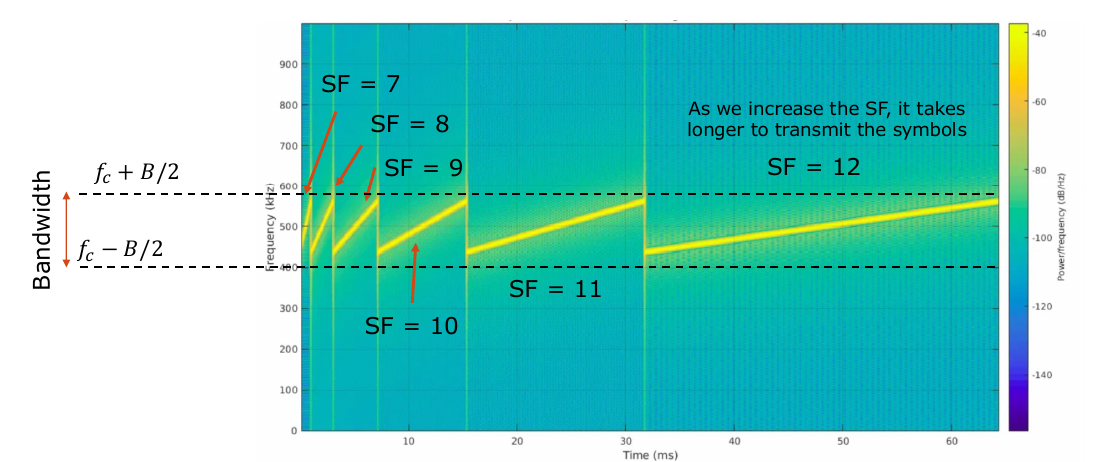
\includegraphics[width=0.8\textwidth]{Pictures/Pasted image 20251028095854.png}
\end{figure}}
\#\#\# Spreading Factor Orthogonality * \textbf{Pseudo-Orthogonal SFs:}
LoRa \(\text{SF}\) values are pseudo-orthogonal. This allows multiple
signals using different data rates (i.e., different \(\text{SF}\)s) to
be transmitted on the same channel and received simultaneously by the
gateway without causing a collision. * \textbf{Collision Resistance:}
Signals using the same \(\text{SF}\) can still be received without
collision if their power difference is \(\ge 6 \text{ dB}\).

\subsection{Code Rate (CR)}\label{code-rate-cr}

\begin{itemize}
\tightlist
\item
  \textbf{Forward Error Correction (FEC):} LoRa employs FEC using a Code
  Rate (\(\text{CR}\)), which adds a number of extra bits every 4 bits,
  with \(\text{CR}\) ranging from 1 to 4.
\item
  \textbf{Actual Bit Rate:} The final, actual bit rate is calculated by
  including the \(\text{CR}\) correction in the formula:
  \[R = \text{SF} \cdot \frac{B}{2^{\text{SF}}} \cdot \left(\frac{4}{4+\text{CR}}\right)\]
  \# LoRa Physical (PHY) Layer: Sensitivity and Adaptive Data Rate (ADR)
\end{itemize}

\section{Sensitivity}\label{sensitivity}

\begin{itemize}
\tightlist
\item
  \textbf{SF and Sensitivity:} Higher \(\text{SF}\) values lead to a
  longer transmission duration (Time on Air, \(\text{ToA}\)). This
  allows the receiver to ``accumulate'' energy for a longer time.

  \begin{itemize}
  \tightlist
  \item
    \textbf{Better Sensitivity:} The result is \textbf{better
    sensitivity}---the receiver is capable of effectively receiving more
    corrupted signals. This translates to a longer communication range
    because the receiver can successfully receive over a more attenuated
    link.
  \item
    \textbf{Minimum SNR:} The required minimum Signal-to-Noise Ratio
    (\(\text{SNR}_m\)) decreases as the \(\text{SF}\) increases. For
    instance, \(\text{SF}7\) requires \(-7.5 \text{ dB}\), while
    \(\text{SF}12\) requires \(-20 \text{ dB}\). (transmitting for a
    longer amount of time, with higher consumption and lower SNR)
  \end{itemize}
\end{itemize}

\section{Data Rate and Trade-offs}\label{data-rate-and-trade-offs}

The trade-off between \(\text{SF}\) and performance parameters is key: *
\textbf{Higher \(\text{SF}\)} leads to a \textbf{Lower bit/data rate}, a
\textbf{Higher \(\text{ToA}\)}, and a \textbf{Higher range}. * The
maximum allowed payload size at the application layer decreases as the
\(\text{SF}\) increases to help reduce the \(\text{ToA}\).

A summary of the trade-offs (for \(\text{BW}=125 \text{ KHz}\) and
\(\text{CR}=1\)) is provided:

\begin{longtable}[]{@{}
  >{\raggedright\arraybackslash}p{(\linewidth - 14\tabcolsep) * \real{0.1250}}
  >{\raggedright\arraybackslash}p{(\linewidth - 14\tabcolsep) * \real{0.1250}}
  >{\raggedright\arraybackslash}p{(\linewidth - 14\tabcolsep) * \real{0.1250}}
  >{\raggedright\arraybackslash}p{(\linewidth - 14\tabcolsep) * \real{0.1250}}
  >{\raggedright\arraybackslash}p{(\linewidth - 14\tabcolsep) * \real{0.1250}}
  >{\raggedright\arraybackslash}p{(\linewidth - 14\tabcolsep) * \real{0.1250}}
  >{\raggedright\arraybackslash}p{(\linewidth - 14\tabcolsep) * \real{0.1250}}
  >{\raggedright\arraybackslash}p{(\linewidth - 14\tabcolsep) * \real{0.1250}}@{}}
\toprule\noalign{}
\begin{minipage}[b]{\linewidth}\raggedright
\textbf{SF}
\end{minipage} & \begin{minipage}[b]{\linewidth}\raggedright
\textbf{DR}
\end{minipage} & \begin{minipage}[b]{\linewidth}\raggedright
\textbf{Bandwidth (KHz)}
\end{minipage} & \begin{minipage}[b]{\linewidth}\raggedright
\textbf{Bit rate (Kbit/s) (CR = 1)}
\end{minipage} & \begin{minipage}[b]{\linewidth}\raggedright
\textbf{Range (km)}
\end{minipage} & \begin{minipage}[b]{\linewidth}\raggedright
\textbf{ToA (ms) (10-Byte)}
\end{minipage} & \begin{minipage}[b]{\linewidth}\raggedright
\textbf{Sensitivity (dBm)}
\end{minipage} & \begin{minipage}[b]{\linewidth}\raggedright
\textbf{Max. payload at app. (B)}
\end{minipage} \\
\midrule\noalign{}
\endhead
\bottomrule\noalign{}
\endlastfoot
7 & DR6 & \textbf{250} & 10.9 & 2 & 28 & -120.5 & 222 \\
7 & DR5 & 125 & 5.5 & 2 & 56 & -123 & 222 \\
8 & DR4 & 125 & 3.125 & 4 & 103 & -126 & 222 \\
9 & DR3 & 125 & 1.758 & 6 & 205 & -129 & 115 \\
10 & DR2 & 125 & 0.977 & 8 & 371 & -132 & 51 \\
11 & DR1 & 125 & 0.537 & 10 & 741 & -134.5 & 51 \\
12 & DR0 & 125 & 0.293 & 12+ & 1483 & -137 & 51 \\
\end{longtable}

\section{Adaptive Data Rate (ADR)}\label{adaptive-data-rate-adr}

\begin{itemize}
\tightlist
\item
  \textbf{ADR Mechanism:} The Adaptive Data Rate (ADR) is a mechanism
  used to select the optimal \(\text{SF}\) based on the link conditions.
\item
  \textbf{Objective:} The goal is to jointly optimize the communication
  quality, network capacity, and power consumption. The \(\text{SF}\)
  should be large enough to ensure reach but not too large to waste
  energy.
\item
  \textbf{Logic:}

  \begin{itemize}
  \tightlist
  \item
    If the link margin is high (good signal), the \(\text{SF}\) can be
    \textbf{reduced} (data rate increased).
  \item
    If the link budget is low (poor signal), the \(\text{SF}\) should be
    \textbf{increased} (data rate reduced) to cope with the worse
    \(\text{SNR}\).
  \end{itemize}
\item
  \textbf{Impact of ADR:} As \(\text{SF}\) increases with distance from
  the gateway, the \(\text{ToA}\) also increases, along with power
  consumption. The visualization shows that end devices far from the
  gateway (up to \(14 \text{ km}\)) use \(\text{SF}12\) with the lowest
  bit rate, while those closest to the gateway use \(\text{SF}7\) with
  the highest bit rate.
\end{itemize}

\chapter{LoRa Physical (PHY) Layer: Frame
Structure}\label{lora-physical-phy-layer-frame-structure}

\section{Physical Frame Structure}\label{physical-frame-structure}

The physical frame is composed of several fields, where the payload size
can range from 0 to 255 bytes:

\begin{longtable}[]{@{}
  >{\raggedright\arraybackslash}p{(\linewidth - 4\tabcolsep) * \real{0.3333}}
  >{\raggedright\arraybackslash}p{(\linewidth - 4\tabcolsep) * \real{0.3333}}
  >{\raggedright\arraybackslash}p{(\linewidth - 4\tabcolsep) * \real{0.3333}}@{}}
\toprule\noalign{}
\begin{minipage}[b]{\linewidth}\raggedright
Field
\end{minipage} & \begin{minipage}[b]{\linewidth}\raggedright
Length
\end{minipage} & \begin{minipage}[b]{\linewidth}\raggedright
Description
\end{minipage} \\
\midrule\noalign{}
\endhead
\bottomrule\noalign{}
\endlastfoot
\textbf{Preamble} & \(6-65535\) symbols & A well-known sequence of
up-chirps and down-chirps. Longer preambles increase the likelihood of
packet detection by the receiver. Typically 8 symbols. \\
\textbf{Mandatory Preamble} & \(4.25\) symbols & Used specifically for
synchronization (frame sync and frequency sync). \\
\textbf{Header} & \(8\) symbols (explicit mode) & Contains the payload
length, data rate configuration, and other settings. It is omitted in
implicit mode (e.g., for fixed-length control messages). \\
\textbf{Payload} & \(0-255\) bytes & The data being transmitted. \\
\textbf{CRC} & \(0-2\) bytes & Cyclic Redundancy Check indication for
the payload. \\
\end{longtable}

\section{MAC Payload Structure}\label{mac-payload-structure}

\pandocbounded{\begin{figure}[h]
\centering
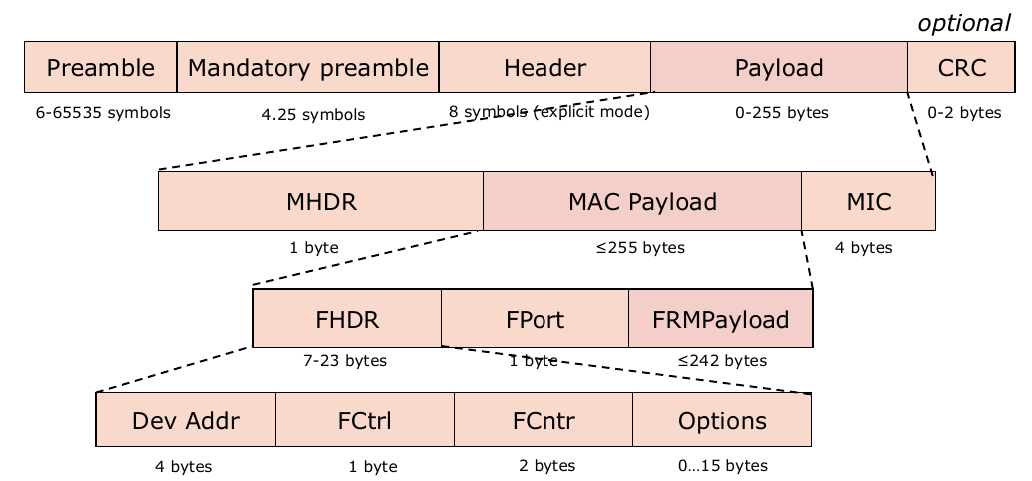
\includegraphics[width=0.8\textwidth]{Pictures/Pasted image 20251029090949.png}
\end{figure}}
The \textbf{Payload} field in the physical frame is actually the
encrypted MAC Payload, which has its own internal structure:

\begin{enumerate}
\def\labelenumi{\arabic{enumi}.}
\tightlist
\item
  \textbf{MHDR (MAC Header):} 1 byte. Specifies the message type (e.g.,
  join-request, data up/down).
\item
  \textbf{MAC Payload:} This section has a maximum size of \(\le 255\)
  bytes and contains the core data and control information. It is
  composed of:

  \begin{itemize}
  \tightlist
  \item
    \textbf{FHDR (Frame Header):} \(7-23\) bytes. Contains key
    addressing and control information:

    \begin{itemize}
    \tightlist
    \item
      \textbf{DevAddr:} (32 bits / 4 bytes) The device address.
    \item
      \textbf{FCtrl (Frame Control):} 1 byte. Contains flags, such as
      whether to use the data rate specified by the gateway for uplink,
      whether the message acknowledges the reception of a previous
      message, or if the gateway has more data for the mote.
    \item
      \textbf{FCntr (Frame Counter):} 2 bytes. A sequence number used
      for security and replay protection.
    \item
      \textbf{Options:} \(0...15\) bytes. Used for MAC commands to
      change data rate, power transmission, etc.
    \end{itemize}
  \item
    \textbf{FPort (Frame Port):} 1 byte. Defines the application port
    number. It only exists if application data is present.
  \item
    \textbf{FRMPayload (Frame Payload):} \(\le 242\) bytes. This is the
    application data itself.
  \end{itemize}
\item
  \textbf{MIC (Message Integrity Code):} 4 bytes. A digital signature
  used for security.
\end{enumerate}

The minimum header of the MAC payload is 12 bytes (MHDR + FHDR + MIC),
plus 1 byte for FPort if application data is sent.

\chapter{LoRa Time on Air (ToA) and Transmission
Examples}\label{lora-time-on-air-toa-and-transmission-examples}

\section{Time on Air (ToA)
Calculation}\label{time-on-air-toa-calculation}

The Time on Air (\(\text{ToA}\)) is the total time required to transmit
a frame, calculated as the sum of the preamble time and the payload
time: \(\text{ToA} = t_{\text{preamble}} + t_{\text{payload}}\).

\begin{itemize}
\tightlist
\item
  \textbf{Preamble Time:}
  \(t_{\text{preamble}} = (n_{\text{preamble}} + 4.25) \cdot T_s\),
  where \(T_s\) is the symbol duration.
\item
  \textbf{Payload Time:}
  \(t_{\text{payload}} = (n_{\text{payload}}) \cdot T_s\), where
  \(n_{\text{payload}}\) is the number of symbols in the payload.
\end{itemize}

The calculation of \(n_{\text{payload}}\) is complex and depends on many
parameters: * Spreading Factor (\(\text{SF}\)). * Payload bytes
(\(\text{PL}\)). * Header enabled status (\(\text{H}\): implicit or
explicit mode). * Low Data Rate Optimization enabled status
(\(\text{DE}\)). * Code Rate (\(\text{CR}\)).

The full formula for \(n_{\text{payload}}\) is derived from the Semtech
SX1276 datasheet:
\[n_{\text{payload}} = 8 + \max\left(\left[\frac{8\text{PL} - 4\text{SF} + 28 + 16\text{CRC} - 20\text{H}}{4(\text{SF} - 2\text{DE})}\right] \cdot (\text{CR} + 4), 0\right)\]

The overall \(\text{ToA}\) can be expressed in terms of \(\text{SF}\)
and \(B\):
\[\text{ToA} = \frac{2^{\text{SF}}}{B} \cdot \left((n_{\text{preamble}} + 4.25) + n_{\text{payload}}\right)\]

\section{Transmission Time Examples}\label{transmission-time-examples}

The Time on Air is highly dependent on both the Spreading Factor and the
total packet size. For a fixed bandwidth (\(B=125 \text{ KHz}\)) and a
packet size of 50 bytes:

\begin{longtable}[]{@{}lll@{}}
\toprule\noalign{}
DR & SF & ToA (\(\text{ms}\)) \\
\midrule\noalign{}
\endhead
\bottomrule\noalign{}
\endlastfoot
DR5 & 7 & \(97.5 \text{ ms}\) \\
DR4 & 8 & \(174.6 \text{ ms}\) \\
DR3 & 9 & \(328.7 \text{ ms}\) \\
DR2 & 10 & \(616.4 \text{ ms}\) \\
DR1 & 11 & \(1,314.8 \text{ ms}\) \\
DR0 & 12 & \(2,302.0 \text{ ms}\) \\
\end{longtable}

This visualization clearly shows that \textbf{increasing the SF
dramatically increases the Time on Air}, which directly impacts how
often a device can transmit due to regulatory duty cycle limits.

\chapter{LoRa Transmission Times and
Constraints}\label{lora-transmission-times-and-constraints}

\section{Duty Cycle Limitations}\label{duty-cycle-limitations}

LoRaWAN transmissions are subject to strict regulatory constraints,
particularly the duty cycle:

\begin{itemize}
\tightlist
\item
  \textbf{Duty Cycle Rule:} In the European region (EU868), a common
  maximum duty cycle is \textbf{\(1\%\)}. This means the transmitter
  must be silent for \(99\%\) of the time after a transmission. The
  total maximum transmission time is \(36\) seconds per hour.
\item
  \textbf{Impact of ToA on Message Count:} The Time on Air
  (\(\text{ToA}\)) dramatically limits the number of messages that can
  be sent per hour:

  \begin{itemize}
  \tightlist
  \item
    \textbf{High Data Rate Example (\(\text{SF}7\)):}

    \begin{itemize}
    \tightlist
    \item
      \(\text{ToA}\) for a \(100 \text{ B}\) packet is
      \(189.7 \text{ ms}\).
    \item
      The required silent time is \(18.78 \text{ seconds}\).
    \item
      Total cycle time is \(\sim 18.97 \text{ s}\).
    \item
      A device can send \(\sim 190\) packets per hour (of
      \(100 \text{ B}\)).
    \end{itemize}
  \item
    \textbf{Low Data Rate Example (\(\text{SF}12\)):}

    \begin{itemize}
    \tightlist
    \item
      \(\text{ToA}\) for a \(100 \text{ B}\) packet is
      \(4431.9 \text{ ms}\) (approx. \(4.43 \text{ s}\)).
    \item
      The required silent time is \(438.7 \text{ seconds}\) (approx.
      \(7.3 \text{ minutes}\)).
    \item
      Total cycle time is \(\sim 443.2 \text{ s}\).
    \item
      A device can send only \(\sim 8\) packets per hour (of
      \(100 \text{ B}\)).
    \end{itemize}
  \end{itemize}
\end{itemize}

\section{Fair Access Policy}\label{fair-access-policy}

In addition to the regulatory duty cycle, some network operators, such
as The Things Network, implement a ``Fair Access Policy'' that further
restricts usage:

\begin{itemize}
\tightlist
\item
  \textbf{Policy Limit:} This policy caps the average uplink Time on Air
  to \textbf{30 seconds per 24 hours per device}. This is a much
  stricter limit than the \(1\%\) duty cycle (\(\sim 36\) seconds per
  hour).
\item
  \textbf{Consequence:} This policy effectively limits the number of
  messages a device can send per day to a very low number, particularly
  at high \(\text{SF}\)s.
\end{itemize}

A useful website:
https://avbentem.github.io/airtime-calculator/ttn/eu868/100

The Fair Access Policy acts as a further constraint beyond the
regulatory duty cycle: * \textbf{Uplink Limit:} An average of \textbf{30
seconds of uplink Time on Air per 24 hours per device}. *
\textbf{Effective Duty Cycle:} This constraint is much stricter,
equating to approximately \(1.25 \text{ seconds/hour}\) (compared to
\(36 \text{ seconds/hour}\) for the \(1\%\) duty cycle). *
\textbf{Downlink Limit:} At most \textbf{10 downlink messages per 24
hours}, which includes \(\text{ACK}\)s for confirmed uplinks. *
\textbf{Message Limits under FAP:} This policy drastically reduces the
number of messages a device can send per day: * High Data Rate
(\(\text{SF}7\), \(100 \text{ B}\)
\(\text{ToA} \approx 189.7 \text{ ms}\)): \(\sim 158\) packets per day.
* Low Data Rate (\(\text{SF}12\), \(100 \text{ B}\)
\(\text{ToA} \approx 4.43 \text{ s}\)): \(\sim 6\) packets per day.

\section{LoRaWAN Architecture}\label{lorawan-architecture}

LoRaWAN defines the components and recommended protocols for the
network, which uses a \textbf{star-of-stars topology}.

The architecture involves four main components: 1. \textbf{End Nodes:}
End devices that perform sensing and actuating tasks. Each is identified
by a \(\text{DevEUI}\) (64 bits). 2. \textbf{Gateway (Concentrator):}
Wireless base stations that receive messages from all End Nodes within
range, based on the LoRa physical layer. They relay the messages to the
Network Server using a backhaul link (e.g., \(4\text{G}\),
\(\text{xDSL}\), Ethernet). Each is identified by a \(\text{DevAddr}\)
(32 bits). 3. \textbf{Network Server:} The central element that: *
Eliminates duplicate messages (since End Nodes transmit messages that
can be received by multiple gateways). * Routes data. * Determines the
optimal data rate (using \(\text{ADR}\)). * Selects the best Gateway to
reach the End Node in Downlink (\(\text{DL}\)) transmissions based on
link quality. 4. \textbf{Application Server:} The final destination for
application data.

\textbf{Security:} The system provides two layers of \(\text{AES}\)
security: * \textbf{Network Session \(\text{AES}\) secured messages}
between the End Node and Network Server. * \textbf{End-to-End
\(\text{AES}\) secured payload} between the End Node and Application
Server.

\chapter{LoRaWAN End Node Classes and Channel
Access}\label{lorawan-end-node-classes-and-channel-access}

\section{Types of End Nodes (Classes A, B, and
C)}\label{types-of-end-nodes-classes-a-b-and-c}

LoRaWAN defines three distinct classes of End Nodes that dictate their
bi-directional communication capabilities and, consequently, their
energy consumption:

\subsection{1. Class A (Base Class)}\label{class-a-base-class}

\begin{itemize}
\tightlist
\item
  \textbf{Communication:} Always initiated by the End Node (UL message
  is completely unsolicited and asynchronous).
\item
  \textbf{Downlink (DL):} After sending an UL message, the End Node
  opens two short receive windows: \(\text{RX}1\) and \(\text{RX}2\).
  The \(\text{DL}\) communication (e.g., commands or \(\text{ACK}\))
  occurs during these windows. If the Network Server doesn't respond in
  \(\text{RX}1\), it tries \(\text{RX}2\). If neither responds,
  \(\text{DL}\) must wait for the next \(\text{UL}\) transmission.
\item
  \textbf{Energy/Latency:} \textbf{Very low energy consumption} (most of
  the time in sleep mode) but \textbf{very large \(\text{DL}\) latency}.
\item
  \textbf{Use Case:} Periodic sensor measurements.
\end{itemize}

\subsection{2. Class B (Bi-directional
Class)}\label{class-b-bi-directional-class}

\begin{itemize}
\tightlist
\item
  \textbf{Communication:} Operates as \(\text{Class A}\) (with
  \(\text{RX}1\) and \(\text{RX}2\)) but adds time-synchronized receive
  windows.
\item
  \textbf{Downlink (DL):} The Gateway sends \textbf{beacons} every
  \(128 \text{ seconds}\). The End Node uses these beacons for
  synchronization to open dedicated \textbf{ping slots (\(\text{PS}\))}.
  These ping slots, which last \(30 \text{ ms}\) each, allow the Gateway
  to initiate \(\text{DL}\) transmissions.
\item
  \textbf{Energy/Latency:} \textbf{Lower (bounded) \(\text{DL}\)
  latency} ( \(\text{DL}\) does not necessarily depend on \(\text{UL}\)
  transmission) but \textbf{higher energy consumption} than
  \(\text{Class A}\).
\item
  \textbf{Use Case:} Utility meters (electrical, water), street lights.
\end{itemize}

\subsection{3. Class C (Continuous Receive
Class)}\label{class-c-continuous-receive-class}

\begin{itemize}
\tightlist
\item
  \textbf{Communication:} Operates as \(\text{Class A}\), but the second
  receive window (\(\text{RX}2\)) remains \textbf{open continuously}
  until the next \(\text{UL}\) transmission.
\item
  \textbf{Downlink (DL):} \(\text{DL}\) messages can be received at
  almost any time via \(\text{RX}2\).
\item
  \textbf{Energy/Latency:} \textbf{Very low \(\text{DL}\) latency} but
  \textbf{very high energy consumption}.
\item
  \textbf{Constraint:} \(\text{Class C}\) devices are generally required
  to be connected to the mains (not battery powered).
\item
  \textbf{Use Case:} Beacon lights, alarms.
\end{itemize}

\section{Channel Access Mechanism}\label{channel-access-mechanism}

\begin{itemize}
\tightlist
\item
  \textbf{Mechanism:} LoRaWAN relies on a random-access scheme known as
  \textbf{Pure ALOHA}.
\item
  \textbf{Operation:} Each End Device transmits whenever it has data to
  send, with \textbf{no coordination} among nodes.
\item
  \textbf{Collision Mitigation:} While collisions can occur, overlapping
  transmissions can still be decoded because the Spreading Factors
  (\(\text{SF}\)s) are quasi-orthogonal.
\end{itemize}


% --- Chapter from 09. NB-IoT.md ---
\section{Executive Summary}\label{executive-summary}

NarrowBand-IoT (NB-IoT) is a cellular technology standardized by the
3GPP, specifically engineered to address the unique requirements of the
Internet of Things (IoT). It leverages existing public cellular
infrastructure (4G-LTE and 5G-NR) to provide a low-power, wide-area
network (LPWAN) solution. Designed for low complexity and minimal
resource consumption in terms of power and spectrum, NB-IoT is
positioned as a leading solution for massive IoT deployments.

The technology operates in licensed frequency bands and offers three
distinct deployment modes---Standalone, In-band, and
Guard-band---allowing for flexible integration into new or existing
cellular networks. Key features include advanced power-saving mechanisms
like Power-Saving Mode (PSM) and Extended Idle Mode DRX (eDRX), which
significantly extend the battery life of endpoint devices. To ensure
robust connectivity in challenging environments, NB-IoT employs a
repetition mechanism, dynamically adjusting data transmissions to
achieve a maximum coupling loss (MCL) of 164 dB, enabling deep indoor
and wide-area coverage of up to 10 km. Data rates are optimized for
typical IoT messaging, with effective throughputs reaching up to 62.5
Kbps in the uplink and 26.2 Kbps in the downlink.

\section{1. Introduction and Core
Concepts}\label{introduction-and-core-concepts}

The proliferation of IoT devices necessitates wireless solutions that
differ significantly from traditional cellular networks, which are
optimized for high bitrates and not power efficiency. NB-IoT was
developed as a specifically designed, cellular-based solution to fill
this gap, offering a more efficient alternative to adapting existing 3G
or 4G protocols.

\textbf{Core Design Principles:}

\begin{itemize}
\tightlist
\item
  \textbf{Standardization:} NB-IoT is standardized by the 3rd Generation
  Partnership Project (3GPP), the body responsible for major mobile
  telecommunications standards.
\item
  \textbf{Foundation:} It is based on the design principles of 4G-LTE,
  such as Orthogonal Frequency Division Multiple Access (OFDMA), but is
  not directly compatible, requiring its own dedicated radio access with
  unique control signals and channels.
\item
  \textbf{Objectives:} The primary targets are low device complexity,
  minimal power consumption, and efficient use of spectrum.
\end{itemize}

\subsection{1.1. Key Applications}\label{key-applications}

NB-IoT is suitable for a wide range of applications that require
long-range, low-power communication for sending small amounts of data.

\begin{itemize}
\tightlist
\item
  \textbf{Smart Agriculture:} Collection of soil and environmental data.
\item
  \textbf{Healthcare Monitoring:} Real-time transmission of vital health
  data from remote monitoring devices.
\item
  \textbf{Retail:} Inventory management, asset security, and enhancement
  of customer experiences.
\item
  \textbf{Energy Management:} Smart meters providing real-time data on
  electricity consumption to improve efficiency.
\item
  \textbf{Supply Chain and Logistics:} Asset tracking and monitoring.
\item
  \textbf{Public Safety:} Connectivity for safety and emergency services
  infrastructure.
\end{itemize}

\section{2. Technical Architecture and
Specifications}\label{technical-architecture-and-specifications}

\subsection{2.1. Frequency Spectrum and
Bands}\label{frequency-spectrum-and-bands}

NB-IoT operates in licensed frequency bands, using the same bands as LTE
but typically favoring the lower range to increase signal range. The use
of licensed spectrum distinguishes it from technologies like LoRa, which
operate in unlicensed bands.

\textbf{LTE Bands for NB-IoT by Region}

\begin{longtable}[]{@{}ll@{}}
\toprule\noalign{}
\endhead
\bottomrule\noalign{}
\endlastfoot
Region & LTE Bands \\
EU & 3, 8, 20 \\
Commonwealth of Independent States & 3, 8, 20 \\
North America & 2, 4, 5, 12, 66, 71, 26 \\
Asia Pacific & 1, 3, 5, 8, 18, 20, 26, 28 \\
Sub-Saharan Africa & 3, 8 \\
Middle East and North Africa & 8, 20 \\
Latin America & 2, 3, 5, 28 \\
\end{longtable}

\textbf{Frequency Range Detail (Europe)}

\begin{longtable}[]{@{}lllll@{}}
\toprule\noalign{}
\endhead
\bottomrule\noalign{}
\endlastfoot
NB-IoT Band & Uplink Band & Downlink Band & Bandwidth & Duplex Mode \\
3 & 1710 - 1785 MHz & 1805 - 1880 MHz & 75 MHz & HD-FDD \\
8 & 880 - 915 MHz & 925 - 960 MHz & 25 MHz & HD-FDD \\
20 & 832 - 862 MHz & 791 - 821 MHz & 30 MHz & HD-FDD \\
\end{longtable}

\subsection{2.2. Deployment and Operation
Modes}\label{deployment-and-operation-modes}

NB-IoT supports three primary operation modes for flexible deployment:

\begin{enumerate}
\def\labelenumi{\arabic{enumi}.}
\tightlist
\item
  \textbf{Standalone:} This mode uses dedicated spectrum, often by
  ``refarming'' spectrum previously used by GSM networks. The NB-IoT
  signal occupies a 180 kHz channel within a 200 kHz GSM carrier, with
  10 kHz guard bands on each side. It is ideal for areas without
  existing cellular network coverage and does not compete with mobile
  broadband services.
\item
  \textbf{In-band:} The NB-IoT signal occupies one 180-kHz Physical
  Resource Block (PRB) within a wider LTE carrier (typically 1.4--20
  MHz). This is considered the most privileged mode due to its
  cost-effectiveness and ease of integration into legacy LTE networks.
  The specific PRBs are predefined to avoid interference with essential
  LTE channels.
\item
  \textbf{Guard-band:} The NB-IoT signal occupies an unused PRB within
  the guard band of an LTE carrier. This allows NB-IoT to coexist with
  primary LTE services without consuming LTE resources, though careful
  configuration is required to mitigate potential out-of-band
  interference. Guard-bands should be as small as possible.
\end{enumerate}

\subsection{2.3. Physical Layer (PHY)}\label{physical-layer-phy}

The NB-IoT physical layer adheres to LTE design principles while being
optimized for IoT use cases.

\begin{itemize}
\tightlist
\item
  \textbf{Multiple Access Scheme:} Orthogonal Frequency Division
  Multiple Access (OFDMA).
\item
  \textbf{Modulation:} QPSK or BPSK.
\item
  \textbf{Transmit Power:} 23 dBm.
\item
  \textbf{Duplexing:} Frequency Division Duplex (FDD) mode only, with
  half-duplex operation (devices can only transmit or receive at any
  given time, not both).
\item
  \textbf{Maximum Transport Block Size (TBS):} 1000 bits for uplink and
  680 bits for downlink.
\end{itemize}

\subsubsection{Frame Structure}\label{frame-structure}

\begin{itemize}
\tightlist
\item
  \textbf{Time Domain:} A 10 ms frame is divided into ten 1 ms
  subframes. Each subframe contains two 0.5 ms slots.
\item
  \textbf{Frequency Domain:} The fundamental unit is a Physical Resource
  Block (PRB), which consists of 12 subcarriers with 15 kHz spacing, for
  a total bandwidth of 180 kHz.
  \pandocbounded{\begin{figure}[h]
\centering
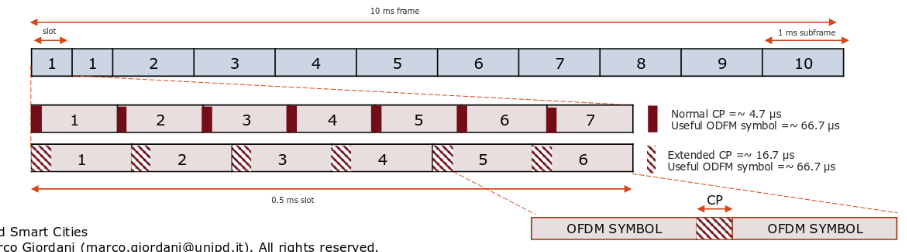
\includegraphics[width=0.8\textwidth]{Pictures/Pasted image 20251105090613.png}
\end{figure}}
\end{itemize}

The more symbol we assign, the better. More opportunities to transmit
data. - Each symbol is separated by Guard- band to avoid inter symbol
interference. \#\#\#\# Uplink Transmission

\begin{itemize}
\tightlist
\item
  \textbf{Single-Tone Transmission:} Each User Equipment (UE) uses only
  one subcarrier (with either 3.75 kHz or 15 kHz spacing). This
  narrowband approach results in low noise power and high
  Signal-to-Noise Ratio (SNR), providing robust and wide coverage, but
  with longer time to transmit.
\item
  \textbf{Multi-Tone Transmission:} UEs can use multiple subcarriers
  (tones) simultaneously, each with 15kHz spacing (3, 6, or 12 tones) to
  increase data rates, reduce transmission delays, and lower power
  consumption by completing transmissions faster.
\end{itemize}

\subsubsection{Uplink Resource Unit (RU)}\label{uplink-resource-unit-ru}

NB-IoT defines a Resource Unit (RU) as a combination of subcarriers
(frequency) and slots (time) for uplink resource mapping. The
configuration of an RU varies based on subcarrier spacing and the number
of tones used.

\begin{longtable}[]{@{}
  >{\raggedright\arraybackslash}p{(\linewidth - 10\tabcolsep) * \real{0.1667}}
  >{\raggedright\arraybackslash}p{(\linewidth - 10\tabcolsep) * \real{0.1667}}
  >{\raggedright\arraybackslash}p{(\linewidth - 10\tabcolsep) * \real{0.1667}}
  >{\raggedright\arraybackslash}p{(\linewidth - 10\tabcolsep) * \real{0.1667}}
  >{\raggedright\arraybackslash}p{(\linewidth - 10\tabcolsep) * \real{0.1667}}
  >{\raggedright\arraybackslash}p{(\linewidth - 10\tabcolsep) * \real{0.1667}}@{}}
\toprule\noalign{}
\endhead
\bottomrule\noalign{}
\endlastfoot
Subcarrier Spacing & \# tones in RU (subcarriers) & \# slots in RU & \#
symbols in slot & Slot duration & RU duration \\
3.75 KHz & 1 & 16 & 7 (normal CP) & 2 ms & 32 ms \\
15 KHz & 1 & 16 & 7 (normal CP) & 0.5 ms & 8 ms \\
15 KHz & 3 & 8 & 7 (normal CP) & 0.5 ms & 4 ms \\
15 KHz & 6 & 4 & 7 (normal CP) & 0.5 ms & 2 ms \\
15 KHz & 12 & 2 & 7 (normal CP) & 0.5 ms & 1 ms \\
\end{longtable}

\subsection{2.4. MAC Layer Features}\label{mac-layer-features}

The MAC layer introduces features critical for extending battery life
and ensuring reliable coverage.

\subsubsection{Power-Saving Mode (PSM)}\label{power-saving-mode-psm}

PSM allows a device to enter a deep-sleep state, disabling parts of its
protocol stack to reduce power consumption to the micro-Ampere range.
The device remains registered with the network, so a reattachment
procedure is not required upon waking, saving significant energy. Two
timers govern this mode:

\begin{itemize}
\tightlist
\item
  \textbf{PSM Active Timer (T3324):} The time a device stays in Idle
  Mode and is reachable for paging.
\item
  \textbf{TAU Timer (T3412):} The time between Tracking Area Updates,
  defining the long sleep period.
\end{itemize}

\subsubsection{Extended Idle Mode DRX
(eDRX)}\label{extended-idle-mode-drx-edrx}

eDRX allows a device to enter a sleep mode while periodically waking to
monitor the network for paging messages. The ``eDRX cycle'' can range
from seconds to minutes. This is suitable for applications that need to
receive data more frequently than PSM allows but do not require constant
connectivity. eDRX can be used in conjunction with PSM, where the device
performs eDRX cycles during the PSM Active Timer (T3324) period.
\pandocbounded{\begin{figure}[h]
\centering
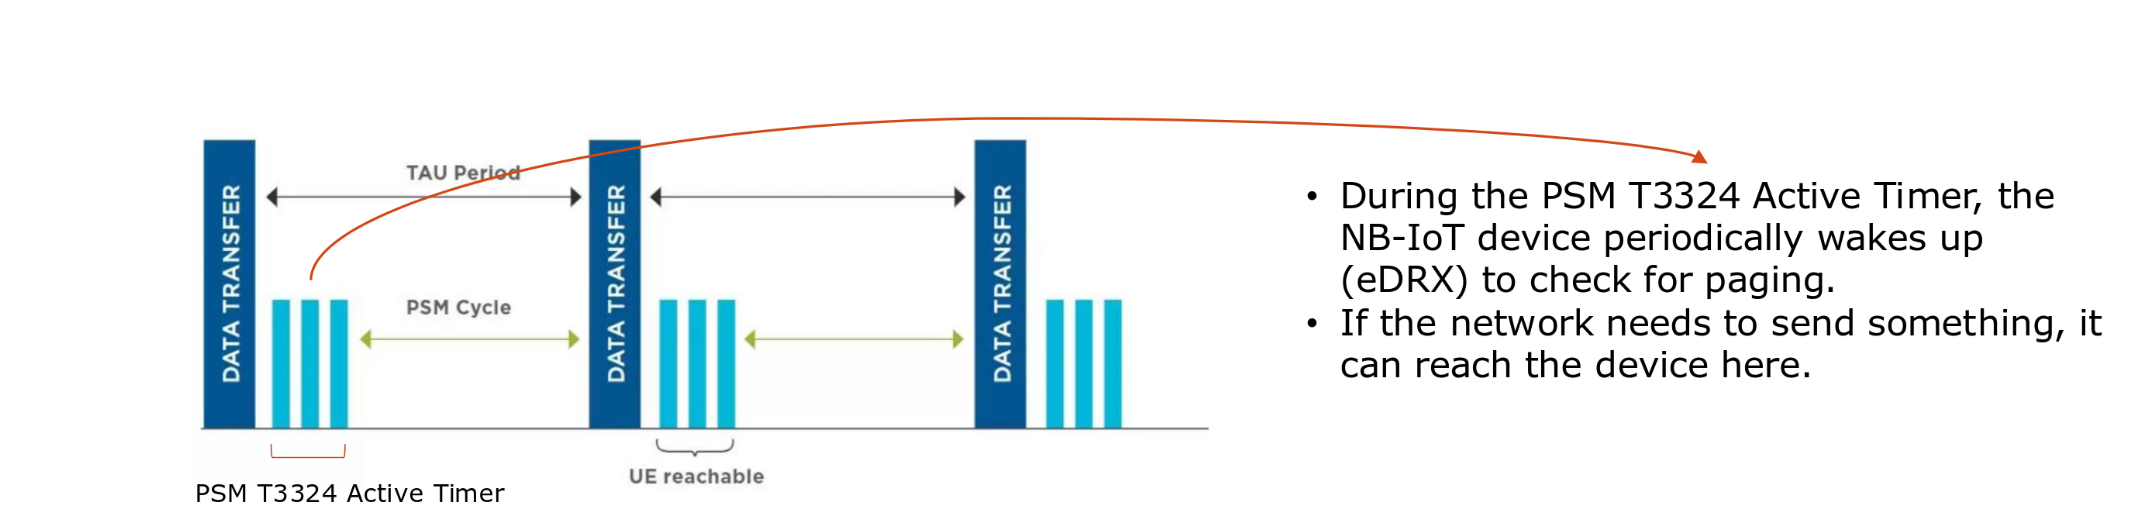
\includegraphics[width=0.8\textwidth]{Pictures/Pasted image 20251105094927.png}
\end{figure}}

\subsubsection{Repetition and Coverage
Extension}\label{repetition-and-coverage-extension}

To operate at the cell edge and in difficult radio environments, NB-IoT
uses repetition.

\begin{itemize}
\tightlist
\item
  \textbf{Mechanism:} Data transmissions are repeated up to 128 times in
  the uplink and 2048 times in the downlink.
\item
  \textbf{Benefit:} Each doubling of repetitions improves receiver
  sensitivity by approximately 3 dB, extending coverage up to 10 km.
\item
  \textbf{Control:} The number of repetitions is dynamically adjusted
  via an \textbf{Enhanced Coverage Level (ECL)} assigned to each device
  based on signal strength. A higher ECL indicates more challenging
  radio conditions and triggers a higher number of repetitions. This
  creates a trade-off between latency (more repetitions take more time)
  and sensitivity.
\end{itemize}

\section{3. Performance Analysis}\label{performance-analysis}

\subsection{3.1. Link Budget and
Coverage}\label{link-budget-and-coverage}

The coverage performance of a wireless network is evaluated using
Maximum Coupling Loss (MCL), which represents the maximum tolerable
signal path loss between the transmitter and receiver. 3GPP sets the
target MCL for NB-IoT at \textbf{164 dB}, indicating superior coverage
capabilities.

\textbf{Link Budget Calculation Example (Single Tone)}

\begin{longtable}[]{@{}lll@{}}
\toprule\noalign{}
\endhead
\bottomrule\noalign{}
\endlastfoot
Parameter & 15 KHz & 3.75 KHz \\
(1) Transmit power (dBm) & 23.0 & 23.0 \\
(2) Thermal noise density (dBm/Hz) & -174 & -174 \\
(3) Receiver noise figure (dB) & 3 & 3 \\
(4) Occupied channel bandwidth (Hz) & 15000 & 3750 \\
(5) Effective noise power (dBm) & -129.2 & -135.3 \\
(6) Required SNR (dB) & -11.8 & -5.7 \\
(7) Receiver sensitivity (S) (dBm) & -141.0 & -141.0 \\
\textbf{(8) Max coupling loss = (1) - (7) (dB)} & \textbf{164.0} &
\textbf{164.0} \\
\end{longtable}

\textbf{MCL Comparison with Other Technologies}

\begin{longtable}[]{@{}ll@{}}
\toprule\noalign{}
\endhead
\bottomrule\noalign{}
\endlastfoot
Radio Access Technology & Maximum Coupling Loss (MCL) {[}dB{]} \\
\textbf{NB-IoT} & \textbf{\textasciitilde{} 164 dB} \\
E-GPRS & \textasciitilde{} 164 dB \\
Sigfox & \textasciitilde{} 162 dB \\
LTE-M & \textasciitilde{} 160 dB \\
LoRa & \textasciitilde{} 157 dB \\
LTE & \textasciitilde{} 144 dB \\
\end{longtable}

\subsection{3.2. Data Rate Capabilities}\label{data-rate-capabilities}

NB-IoT data rates are calculated based on the transport block size, the
number of Resource Units (or subframes), the duration of these units,
and scheduling overhead.

\begin{itemize}
\tightlist
\item
  \textbf{Uplink (Single-Tone):}

  \begin{itemize}
  \tightlist
  \item
    Minimum time to transmit 1000 bits: 48 ms.
  \item
    Peak PHY Data Rate: 1000 bits / 48 ms = \textbf{20.8 Kbps}.
  \item
    Effective Data Rate (with scheduling overhead): 1000 bits / (48+12)
    ms = \textbf{16.7 Kbps}.
  \end{itemize}
\item
  \textbf{Uplink (Multi-Tone):}

  \begin{itemize}
  \tightlist
  \item
    Minimum time to transmit 1000 bits: 4 ms.
  \item
    Peak PHY Data Rate: 1000 bits / 4 ms = \textbf{250 Kbps}.
  \item
    Effective Data Rate (with scheduling overhead): 1000 bits / (4+12)
    ms = \textbf{62.5 Kbps}.
  \end{itemize}
\item
  \textbf{Downlink:}

  \begin{itemize}
  \tightlist
  \item
    Minimum time to transmit 680 bits: 4 ms.
  \item
    Peak PHY Data Rate: 680 bits / 4 ms = \textbf{170 Kbps}.
  \item
    Effective Data Rate (with scheduling overhead): 680 bits / (4+22) ms
    = \textbf{26.2 Kbps}.
  \end{itemize}
\end{itemize}


% --- Chapter from 10. WebSocket.md ---
\section{Executive Summary}\label{executive-summary}

The complex requirements of modern Internet of Things (IoT)
applications---including real-time data exchange, large-scale
deployments, and device constraints---necessitate specialized
application-layer protocols that extend beyond the capabilities of
standard TCP and UDP. While the HyperText Transfer Protocol (HTTP) forms
the backbone of the traditional web, its strict, half-duplex,
request-response model is ill-suited for the dynamic, event-driven
nature of IoT. Key limitations of HTTP include its inability to support
unsolicited server-side updates, its high overhead from verbose textual
headers, and the complexity of options not required by many IoT use
cases.

WebSocket emerges as a more efficient alternative, specifically designed
to address these shortcomings. It establishes a persistent, full-duplex,
bidirectional TCP connection between a client and a server through an
initial HTTP handshake. This allows for low-latency, unsolicited data
exchange from either endpoint with minimal overhead after the connection
is established. The protocol's efficiency is further enhanced by a
minimal frame header structure. However, despite its advantages for
real-time communication, WebSocket remains fundamentally a client-server
protocol. For certain large-scale IoT scenarios, more tailored solutions
based on the publish-subscribe paradigm may prove more effective.

\section{The Middleware Imperative in
IoT}\label{the-middleware-imperative-in-iot}

Standard internet transport protocols like TCP and UDP are foundational
but insufficient on their own to manage the complexity of advanced IoT
and Smart City applications. The unique demands of these environments
require a ``middleware'' layer of application protocols and components
to provide full support.

The need for this middleware is driven by several factors inherent to
IoT systems:

\begin{itemize}
\tightlist
\item
  \textbf{Data Heterogeneity:} IoT networks must handle diverse types of
  data, including notifications, measurements, and commands.
\item
  \textbf{Traffic Diversity:} The system must support both non-real-time
  traffic and traffic with hard real-time requirements.
\item
  \textbf{Architectural Flexibility:} Both client-server and
  publish-subscribe communication models are often required within the
  same system.
\item
  \textbf{Endpoint Constraints:} Many IoT devices have significant
  constraints related to processing power, battery life, and available
  bandwidth.
\item
  \textbf{System Scale:} IoT deployments can be large-scale
  cyber-physical systems requiring robust and efficient management.
\item
  \textbf{Storage Complexity:} The volume and velocity of data generated
  create significant storage challenges.
\end{itemize}

Given these varied and often conflicting requirements, no single
networking solution can satisfy all IoT scenarios.

\section{An Examination of HyperText Transfer Protocol
(HTTP)}\label{an-examination-of-hypertext-transfer-protocol-http}

HTTP is the protocol that underpins the World Wide Web, defining how
client-server programs retrieve web pages. A client (e.g., a browser)
sends a request, and a server returns a response. It typically uses TCP
as its transport protocol, leveraging TCP's reliability to ensure
messages are not lost or corrupted. When combined with Transport Layer
Security (TLS), it becomes HTTPS (HTTP Secure).

\subsection{Resource Identification: The
URL}\label{resource-identification-the-url}

Resources on the web are identified by a Uniform Resource Locator (URL),
which combines four key identifiers:

\begin{itemize}
\tightlist
\item
  \textbf{Protocol:} The client-server application to be used (e.g.,
  \texttt{http}).
\item
  \textbf{Host:} The unique name or IP address of the server.
\item
  \textbf{Port:} The 16-bit port number for the application (e.g., HTTP
  defaults to port 80). It is often omitted if the default is used.
\item
  \textbf{Path:} The location and name of the file on the server's
  operating system (e.g., \texttt{/en/department/map-department}).
\end{itemize}

The standard formats are \texttt{protocol://host/path} or
\texttt{protocol://host:port/path}.

\subsection{HTTP Methods}\label{http-methods}

HTTP operates using a set of request methods that specify the desired
action to be performed on a resource.

\begin{longtable}[]{@{}
  >{\raggedright\arraybackslash}p{(\linewidth - 6\tabcolsep) * \real{0.2500}}
  >{\raggedright\arraybackslash}p{(\linewidth - 6\tabcolsep) * \real{0.2500}}
  >{\raggedright\arraybackslash}p{(\linewidth - 6\tabcolsep) * \real{0.2500}}
  >{\raggedright\arraybackslash}p{(\linewidth - 6\tabcolsep) * \real{0.2500}}@{}}
\toprule\noalign{}
\endhead
\bottomrule\noalign{}
\endlastfoot
Method & Description & Safe & Idempotent \\
\textbf{GET} & Requests a representation of the specified resource. &
Yes & Yes \\
\textbf{HEAD} & Asks for a response identical to a GET request, but
without the response body. & Yes & Yes \\
\textbf{POST} & Submits an entity to the specified resource, often
causing a change in state or side effects on the server. & No & No \\
\textbf{PUT} & Replaces all current representations of the target
resource with the request payload. & No & Yes \\
\textbf{DELETE} & Deletes the specified resource. & No & Yes \\
\textbf{TRACE} & Performs a message loop-back test along the path to the
target resource. & Yes & Yes \\
\textbf{OPTIONS} & Returns the communication options for the target
resource. & Yes & Yes \\
\textbf{CONNECT} & Establishes a tunnel to the server identified by the
target resource. & No & No \\
\textbf{PATCH} & Applies partial modifications to a resource. & No &
No \\
\end{longtable}

\subsection{Critical Limitations for IoT
Applications}\label{critical-limitations-for-iot-applications}

Despite its ubiquity, standard HTTP presents significant problems for
IoT traffic:

\begin{itemize}
\tightlist
\item
  \textbf{Strict Client-Server Model:} Communication is always initiated
  by the client. The server can only respond to a request and cannot
  send unsolicited updates, such as when a sensor's state changes. This
  inability to support asynchronous, server-initiated events is a major
  drawback for IoT.
\item
  \textbf{Verbose Headers:} HTTP headers are textual (UTF-8 encoded) and
  can be very large (in the order of 100 KB), which is inefficient for
  resource-constrained IoT devices and networks.
\item
  \textbf{Unnecessary Complexity:} The protocol includes sophisticated
  options that are often unused in IoT contexts, adding unnecessary
  overhead.
\item
  \textbf{Gateway Inefficiency:} While newer versions like HTTP/2 and
  HTTP/3 offer improvements, standard HTTP is not considered an ideal
  solution for IoT gateway-based networks.
\end{itemize}

\section{WebSocket: A Bidirectional Communication
Protocol}\label{websocket-a-bidirectional-communication-protocol}

For IoT traffic, WebSocket provides a more suitable communication
architecture. It is defined by two core elements:

\begin{enumerate}
\def\labelenumi{\arabic{enumi}.}
\tightlist
\item
  A mechanism to upgrade an initial HTTP connection into a persistent,
  bidirectional TCP connection.
\item
  A minimal set of messages for efficient data transfer and connection
  maintenance.
\end{enumerate}

\subsection{Connection Lifecycle and
Operation}\label{connection-lifecycle-and-operation}

The connection process begins with a client sending a standard HTTP GET
request to a server. If the server supports WebSocket, it agrees to the
protocol upgrade by sending a specific response, and the bidirectional
WebSocket communication can begin. If the server does not support
WebSocket, it returns a standard HTTP error code.

Once established, the connection is symmetrical, allowing either the
client or the server to send unsolicited messages at any time. This
full-duplex capability is a key advantage over HTTP for event-driven IoT
applications.

\subsection{Efficient Frame Structure}\label{efficient-frame-structure}

To minimize overhead, WebSocket messages use a compact binary frame
structure with a minimal header.

\begin{longtable}[]{@{}
  >{\raggedright\arraybackslash}p{(\linewidth - 4\tabcolsep) * \real{0.3333}}
  >{\raggedright\arraybackslash}p{(\linewidth - 4\tabcolsep) * \real{0.3333}}
  >{\raggedright\arraybackslash}p{(\linewidth - 4\tabcolsep) * \real{0.3333}}@{}}
\toprule\noalign{}
\endhead
\bottomrule\noalign{}
\endlastfoot
Field & Size & Description \\
\textbf{F (FIN)} & 1 bit & If set to 1, indicates that this is a
complete message or the final fragment of a fragmented message. \\
\textbf{R (Reserved)} & 3 bits & Reserved for future use. \\
\textbf{Opcode} & 4 bits & Indicates the type of message being sent
(e.g., text, binary, connection close). \\
\textbf{M (Mask)} & 1 bit & If set to 1, a 4-byte \texttt{Mask} field is
present in the header. Masking is mandatory for all client-to-server
communications to prevent cache poisoning attacks. \\
\textbf{L (Length)} & 7 bits & Indicates the payload length. Its
interpretation is variable:  \\
\textbf{Mask} & 4 bytes & \emph{(Optional)} A masking key used to XOR
the payload data. Present only if M=1. \\
\textbf{Payload Data} & Variable & The application data. \\
\end{longtable}

\subsection{Limitations in an IoT
Context}\label{limitations-in-an-iot-context}

While WebSocket significantly improves upon HTTP for real-time IoT
communications, it has a primary limitation: it is still a client-server
model. For many large-scale IoT systems, more effective and tailored
solutions based on the publish-subscribe paradigm may be required.

\section{Comparative Analysis: HTTP
vs.~WebSocket}\label{comparative-analysis-http-vs.-websocket}

The fundamental differences between the two protocols highlight
WebSocket's suitability for modern, interactive applications.

\begin{longtable}[]{@{}
  >{\raggedright\arraybackslash}p{(\linewidth - 4\tabcolsep) * \real{0.3333}}
  >{\raggedright\arraybackslash}p{(\linewidth - 4\tabcolsep) * \real{0.3333}}
  >{\raggedright\arraybackslash}p{(\linewidth - 4\tabcolsep) * \real{0.3333}}@{}}
\toprule\noalign{}
\endhead
\bottomrule\noalign{}
\endlastfoot
Feature & WebSocket & HTTP \\
\textbf{Connection Type} & Full-duplex, persistent connection. &
Half-duplex, request-response model. \\
\textbf{Communication} & Bidirectional & Unidirectional \\
\textbf{Overhead} & Minimal after the initial handshake. & High for
repeated requests. \\
\textbf{Efficiency} & High & Moderate \\
\end{longtable}


% --- Chapter from 11. MQTT.md ---
\section{Executive Summary}\label{executive-summary}

Message Queuing Telemetry Transport (MQTT) is a lightweight,
IoT-specific application protocol engineered for collecting event data
from sensors in environments with constrained devices and potentially
unreliable networks. Layered on TCP or TLS, it operates on a
publish-subscribe paradigm, which decouples message producers
(publishers) from consumers (subscribers) through a central broker. This
architecture avoids direct client-to-client connections and routes
messages based on subscriptions to specific ``topics.''

Key features that define MQTT's utility in IoT include a highly
efficient message frame with a minimal header, a flexible
\textbf{Quality of Service (QoS)} mechanism offering three levels of
message reliability, and specialized functionalities for state
management. \textbf{Retained Messages} allow new subscribers to receive
the most recent value for a topic immediately upon connecting. The
\textbf{Last Will and Testament (LWT)} feature ensures system-wide
notification if a client disconnects ungracefully. While MQTT's design
makes it an excellent choice for embedded platforms, its reliance on a
centralized broker can introduce challenges related to scalability and
reliability.

\section{1. Core Concepts and
Architecture}\label{core-concepts-and-architecture}

MQTT is an application-layer protocol specifically designed for the
Internet of Things, focusing on the efficient collection of data from
sensors. Its architecture is fundamentally different from
request-response protocols like HTTP.

\subsection{Publish-Subscribe
Paradigm}\label{publish-subscribe-paradigm}

The MQTT protocol is implemented based on the publish-subscribe model,
which involves three main components:

\begin{itemize}
\tightlist
\item
  \textbf{Publisher:} A client that sends messages.
\item
  \textbf{Broker:} A central server that receives all messages from
  publishers and distributes them to the appropriate subscribers. It
  acts as the intermediary for all communication.
\item
  \textbf{Subscriber:} A client that registers interest in one or more
  topics and receives messages published to those topics from the
  broker.
\end{itemize}

In this model, subscribers and publishers are decoupled; they do not
need to know about each other's existence and never establish direct
connections. Communication is organized around \textbf{topics}, which
are hierarchical strings that act as message channels.

\section{2. Message Frame Structure}\label{message-frame-structure}

To ensure efficiency on constrained devices, MQTT messages are
characterized by a minimal header structure. The frame consists of a
fixed header, an optional variable header, and an optional payload.

\begin{longtable}[]{@{}
  >{\raggedright\arraybackslash}p{(\linewidth - 4\tabcolsep) * \real{0.3333}}
  >{\raggedright\arraybackslash}p{(\linewidth - 4\tabcolsep) * \real{0.3333}}
  >{\raggedright\arraybackslash}p{(\linewidth - 4\tabcolsep) * \real{0.3333}}@{}}
\toprule\noalign{}
\endhead
\bottomrule\noalign{}
\endlastfoot
Component & Size & Description \\
\textbf{Fixed Header} & & Present in every MQTT message. \\
Packet Type & 4 bits & Defines the type of MQTT message (e.g., CONNECT,
PUBLISH). \\
Control Flags & 4 bits & Specific flags dependent on the packet type. \\
Remaining Length & 1-4 bytes & The length of the rest of the packet
(Variable Header + Payload). \\
\textbf{Variable Header} & N bytes & Optional field present in some
messages. Its content varies by packet type. \\
\textbf{Payload} & M bytes & The final part of the packet. Contains the
application-specific data. \\
\end{longtable}

\subsection{Variable Byte Integer
Encoding}\label{variable-byte-integer-encoding}

The \texttt{Remaining\ Length} field uses a variable-length encoding
scheme called a \textbf{Variable Byte Integer}. This allows the field to
use between one and four bytes, depending on the size of the value it
represents. In each byte, the lower 7 bits encode data, and the most
significant bit (MSB) acts as a ``continuation flag.'' If the MSB is 1,
it indicates that another byte follows; if it is 0, it is the final
byte.

This encoding supports a maximum payload size of nearly 268 MB.

\begin{longtable}[]{@{}lll@{}}
\toprule\noalign{}
\endhead
\bottomrule\noalign{}
\endlastfoot
Bytes Used & Value Range From & Value Range To \\
1 & 0 & 127 \\
2 & 128 & 16,383 \\
3 & 16,384 & 2,097,151 \\
4 & 2,097,152 & 268,435,455 \\
\end{longtable}

\section{3. Key MQTT Message Types}\label{key-mqtt-message-types}

The protocol defines a set of messages for connection management,
subscriptions, and data publication. The core messages examined are
CONNECT, CONNACK, SUBSCRIBE, and PUBLISH.

\subsection{CONNECT}\label{connect}

The \texttt{CONNECT} message is the first packet sent by a client to
open or reopen a session with the broker. It carries the client's unique
ID and various connection flags.

\begin{itemize}
\tightlist
\item
  \textbf{Key Fields in Variable Header:}

  \begin{itemize}
  \tightlist
  \item
    \textbf{Protocol Name \& Version:} Specifies the MQTT protocol
    details.
  \item
    \textbf{Flags:} A single byte containing several 1-bit flags:

    \begin{itemize}
    \tightlist
    \item
      \texttt{Username} \& \texttt{Password}: Indicate if credentials
      are present in the payload.
    \item
      \texttt{Will\ Flag}: If set, the ``Will Message'' fields
      (\texttt{Will\ Topic}, \texttt{Will\ Payload}, \texttt{Will\ QoS},
      \texttt{Will\ Retain}) are included to configure the Last Will and
      Testament feature.
    \item
      \texttt{Clean\ Start}: If set, the broker creates a fresh session
      for the client. If not, it attempts to resume a previous session.
    \end{itemize}
  \item
    \textbf{Keep Alive:} A 2-byte integer specifying the maximum time
    interval (in seconds) that can pass between control packets sent by
    the client. It is used to detect unresponsive clients.
  \end{itemize}
\end{itemize}

\subsection{CONNACK}\label{connack}

The \texttt{CONNACK} message is the server's response to a
\texttt{CONNECT} request, indicating the result of the connection
attempt. It has no payload.

\begin{itemize}
\tightlist
\item
  \textbf{Key Fields in Variable Header:}

  \begin{itemize}
  \tightlist
  \item
    \textbf{Connect Flags:} Contains the \texttt{Session\ Present} flag,
    which informs the client whether the broker is resuming a
    pre-existing session.
  \item
    \textbf{Reason Code:} A 1-byte code indicating the status of the
    connection.
  \end{itemize}
\end{itemize}

\begin{longtable}[]{@{}
  >{\raggedright\arraybackslash}p{(\linewidth - 4\tabcolsep) * \real{0.3333}}
  >{\raggedright\arraybackslash}p{(\linewidth - 4\tabcolsep) * \real{0.3333}}
  >{\raggedright\arraybackslash}p{(\linewidth - 4\tabcolsep) * \real{0.3333}}@{}}
\toprule\noalign{}
\endhead
\bottomrule\noalign{}
\endlastfoot
Value & Reason Code Name & Description \\
\texttt{0x00} & Success & The connection is accepted. \\
\texttt{0x81} & Malformed Packet & The server could not parse the
CONNECT packet. \\
\texttt{0x82} & Protocol Error & The packet was parsed, but its content
violates the protocol. \\
\texttt{0x84} & Unsupported Protocol Version & The server does not
support the client's requested MQTT version. \\
\texttt{0x85} & Client Identifier not valid & The Client ID is
syntactically valid but rejected by the server. \\
\texttt{0x86} & Bad User Name or Password & The provided credentials
were incorrect. \\
\texttt{0x95} & Packet too large & The CONNECT packet exceeds the
server's maximum allowed size. \\
\texttt{0x8A} & Banned & The client is banned from connecting (e.g.,
added to a blacklist). \\
\end{longtable}

\subsection{SUBSCRIBE}\label{subscribe}

The \texttt{SUBSCRIBE} message allows a client to register its interest
in one or more topics. The broker will then forward messages published
to these topics to the client.

\begin{itemize}
\tightlist
\item
  \textbf{Key Fields in Payload:}

  \begin{itemize}
  \tightlist
  \item
    \textbf{Topic Filter(s):} A list of topic strings the client wishes
    to subscribe to.
  \item
    \textbf{Options:} Subscription-specific options for each topic
    filter.

    \begin{itemize}
    \tightlist
    \item
      \texttt{QoS}: Specifies the maximum QoS level at which the server
      can send messages to this client for this subscription.
    \item
      \texttt{Retain\ Handling}: Dictates whether the server should send
      Retained Messages when the subscription is established.
    \item
      \texttt{Retain\ As\ Published}: Indicates if the Retain flag
      should be preserved on messages forwarded to this subscription.
    \item
      \texttt{No\ Local}: If set, the server will not forward messages
      to this client if this same client was the original publisher.
    \end{itemize}
  \end{itemize}
\end{itemize}

\subsection{PUBLISH}\label{publish}

The \texttt{PUBLISH} message is used to distribute application data. It
can be sent from a client to the server (publishing a message) or from
the server to a client (delivering a message).

\begin{itemize}
\tightlist
\item
  \textbf{Key Fields:}

  \begin{itemize}
  \tightlist
  \item
    \textbf{Control Flags:}

    \begin{itemize}
    \tightlist
    \item
      \texttt{DUP}: Set to 1 if the packet is a retransmission of an
      earlier message.
    \item
      \texttt{QoS}: Specifies the Quality of Service level for this
      message.
    \item
      \texttt{Retain}: If set to 1, the broker must store this message
      as the ``last known good'' value for its topic.
    \end{itemize}
  \item
    \textbf{Variable Header:}

    \begin{itemize}
    \tightlist
    \item
      \texttt{Topic\ Name}: The topic channel to which the message is
      being published.
    \item
      \texttt{Packet\ Identifier}: A unique ID required for messages
      with QoS levels 1 and 2.
    \end{itemize}
  \item
    \textbf{Payload:} The actual application message content.
  \end{itemize}
\end{itemize}

\section{4. Advanced Features and
Mechanisms}\label{advanced-features-and-mechanisms}

MQTT includes several features designed to enhance reliability and state
management in dynamic IoT environments.

\subsection{Retained Messages}\label{retained-messages}

When a broker receives a \texttt{PUBLISH} message with the
\texttt{Retain} flag set to 1, it stores that message for the specified
topic. When a new client subscribes to that topic, the broker
immediately sends this stored message to the new subscriber. This allows
clients to get the latest status or value right away, without having to
wait for the publisher to send a new update. This is particularly useful
for sensors monitoring values that change infrequently.

\subsection{Last Will and Testament
(LWT)}\label{last-will-and-testament-lwt}

The LWT is a mechanism for notifying other clients about an ungraceful
disconnection. A client can specify a ``Will Message,'' ``Will Topic,''
and other parameters in its initial \texttt{CONNECT} packet. If the
client's connection terminates unexpectedly (e.g., without a clean
\texttt{DISCONNECT} message or due to a protocol error), the broker will
publish the Will Message to the Will Topic on behalf of the departed
client. This feature can be combined with Retained Messages by setting
the \texttt{Will\ Retain} flag, ensuring the LWT message is stored and
delivered to future subscribers.

\subsection{Keep Alive}\label{keep-alive}

The Keep Alive feature helps both the client and the server detect
half-open TCP connections, where one side believes the connection is
active while the other side has closed it. The client specifies a Keep
Alive interval (in seconds) in the \texttt{CONNECT} message. The client
is then responsible for ensuring it sends at least one MQTT packet
within each interval. If the server does not receive any packets from
the client within 1.5 times the Keep Alive interval, it assumes the
connection is lost, closes it, and publishes the client's LWT message if
one was configured.

\section{5. Quality of Service (QoS)}\label{quality-of-service-qos}

MQTT provides three distinct QoS levels to allow developers to choose
the appropriate level of message delivery reliability for their
application, which is crucial in unstable network environments. The QoS
level is specified in the subscription request.

\begin{itemize}
\tightlist
\item
  \textbf{QoS 0: At Most Once}

  \begin{itemize}
  \tightlist
  \item
    Also known as ``fire and forget.''
  \item
    The message is sent once without any acknowledgment.
  \item
    There is no guarantee of delivery, and messages may be lost.
  \end{itemize}
\item
  \textbf{QoS 1: At Least Once}

  \begin{itemize}
  \tightlist
  \item
    Guarantees that the message will be delivered at least one time.
  \item
    The sender sends a \texttt{PUBLISH} packet and stores it until it
    receives a \texttt{PUBACK} (Publish Acknowledgment) packet from the
    receiver.
  \item
    If no \texttt{PUBACK} is received, the message is retransmitted,
    which can lead to the receiver getting duplicate messages.
  \end{itemize}
\item
  \textbf{QoS 2: Exactly Once}

  \begin{itemize}
  \tightlist
  \item
    The highest level of service, ensuring that each message is received
    exactly once, without loss or duplication.
  \item
    It involves a four-part handshake:

    \begin{enumerate}
    \def\labelenumi{\arabic{enumi}.}
    \tightlist
    \item
      Sender sends \texttt{PUBLISH} and waits for a \texttt{PUBREC}
      (Publish Received).
    \item
      Upon receiving \texttt{PUBREC}, the sender can discard the
      original message and sends a \texttt{PUBREL} (Publish Release).
    \item
      The receiver processes the message and responds with a
      \texttt{PUBCOMP} (Publish Complete).
    \item
      When the sender receives \texttt{PUBCOMP}, the transaction is
      complete.
    \end{enumerate}
  \end{itemize}
\end{itemize}

\section{6. Final Considerations}\label{final-considerations}

MQTT is a highly effective protocol for IoT systems, particularly those
involving constrained endpoints like Arduino or Raspberry Pi.

\subsection{Strengths}\label{strengths}

\begin{itemize}
\tightlist
\item
  \textbf{Lightweight:} The minimal message header makes it efficient
  for low-bandwidth networks and low-power devices.
\item
  \textbf{Platform Support:} It can be implemented on many embedded
  platforms and has numerous open-source implementations available.
\item
  \textbf{State Management:} The Retained Message mechanism allows for
  the seamless addition of new endpoints that can immediately
  synchronize with the system's state.
\item
  \textbf{Reliability Features:} The LWT feature provides robust
  management of connectivity outages.
\end{itemize}

\subsection{Weaknesses}\label{weaknesses}

\begin{itemize}
\tightlist
\item
  \textbf{Centralized Broker:} The primary drawback is its reliance on a
  central broker. This can create a single point of failure and may pose
  scalability and reliability challenges in very large-scale
  deployments.
\end{itemize}


% --- Chapter from 12. CoAP.md ---
\section{Executive Summary}\label{executive-summary}

The Constrained Application Protocol (CoAP) is an application layer
protocol specifically engineered for the Internet of Things (IoT). It is
designed to enable small, low-power devices with limited computational
resources and bandwidth to participate in the broader internet.
Operating on a client-server paradigm similar to HTTP, CoAP utilizes UDP
for transport, necessitating its own mechanisms for error recovery.
Security is managed at the network layer via IPsec or through Datagram
Transport Layer Security (DTLS).

Key features of CoAP include its compact message format,
interoperability with HTTP via gateways, and a unique ``resource
observation'' function that emulates a publish-subscribe model, allowing
clients to receive asynchronous updates on a resource's state. The
protocol distinguishes between \texttt{Message\ ID}s, used for duplicate
detection and acknowledging messages, and \texttt{Token}s, used to match
specific requests with their corresponding responses. While its RESTful
model and simplicity are advantageous for web developers, its
fundamental client-server nature makes MQTT a more suitable choice for
applications requiring a true publish-subscribe architecture.

\begin{center}\rule{0.5\linewidth}{0.5pt}\end{center}

\section{1. Core Concepts and
Architecture}\label{core-concepts-and-architecture}

\subsection{1.1. Protocol Purpose and
Design}\label{protocol-purpose-and-design}

CoAP is an IoT-specific application protocol created to accommodate the
limitations of constrained devices, such as scarce bandwidth, low power,
limited computational capacity, and long sleep times. Its primary goal
is to allow these devices to integrate with the wider internet.

\begin{itemize}
\tightlist
\item
  \textbf{Transport Protocol:} CoAP is layered on top of the User
  Datagram Protocol (UDP), in contrast to protocols like MQTT which
  typically use TCP. This choice necessitates dedicated error recovery
  mechanisms within CoAP itself.
\item
  \textbf{Security:} To provide security, CoAP can utilize IPsec at the
  network layer or Datagram Transport Layer Security (DTLS).
\item
  \textbf{Communication Model:} It is implemented based on the
  client-server paradigm, with communication consisting of a sequence of
  requests (methods) and responses, conceptually similar to HTTP.
  Although not equivalent to HTTP, internetworking between the two
  protocols is designed to be straightforward.
\end{itemize}

\subsection{1.2. System Architecture}\label{system-architecture}

CoAP supports several communication patterns:

\begin{itemize}
\tightlist
\item
  Endpoints (clients) can communicate with a CoAP server.
\item
  Endpoints can communicate with an HTTP server through a gateway.
\item
  Endpoints can communicate directly in a peer-to-peer fashion.
\end{itemize}

A significant feature is that the ``lightweight'' characteristics of the
protocol make it feasible to configure a CoAP server even on
resource-constrained endpoints. Furthermore, a device acting as a CoAP
server may also act as a client.

\section{2. CoAP Frame Structure and
Semantics}\label{coap-frame-structure-and-semantics}

The CoAP message format is designed to be more compact than HTTP's,
though it can be slightly more complex than MQTT's.

\textbf{Header Format:}

\texttt{V\ (2\ bits)\ \textbar{}\ T\ (2\ bits)\ \textbar{}\ TKL\ (4\ bits)\ \textbar{}\ Code\ (1\ byte)\ \textbar{}\ Message\ ID\ (2\ bytes)}
\texttt{Token\ (0-8\ bytes)} \texttt{Options\ (N\ bytes)}
\texttt{Payload\ (K\ bytes)}

\subsection{2.1. Header Fields Explained}\label{header-fields-explained}

\begin{itemize}
\tightlist
\item
  \textbf{Version (V):} 2 bits indicating the CoAP version.
\item
  \textbf{Type (T):} 2 bits defining the message type.

  \begin{itemize}
  \tightlist
  \item
    \textbf{0 - Confirmable (CON):} This message requires an
    acknowledgement message.
  \item
    \textbf{1 - Non-confirmable (NON):} This message does not require
    confirmation.
  \item
    \textbf{2 - Acknowledgement (ACK):} A response that acknowledges a
    Confirmable message.
  \item
    \textbf{3 - Reset (RST):} Indicates the receiver cannot or will not
    process a request.
  \end{itemize}
\item
  \textbf{Token Length (TKL):} 4 bits specifying the length of the Token
  field, which can be 0.
\item
  \textbf{Code:} 1 byte indicating the request method or response code.
  It consists of a 3-bit class and a 5-bit code.
\item
  \textbf{Message ID:} A 2-byte value used to detect duplicate messages
  and retransmissions.
\item
  \textbf{Token:} A variable-length field (0-8 bytes) used to correlate
  a request with its response.
\end{itemize}

\subsection{2.2. Distinguishing Message ID
vs.~Token}\label{distinguishing-message-id-vs.-token}

CoAP uses two separate identifiers for message correlation, each with a
distinct purpose.

\begin{itemize}
\tightlist
\item
  \textbf{Message ID:} This unique value is used to match a
  \textbf{Confirmable (CON)} message to its corresponding
  \textbf{Acknowledgement (ACK)} message. Its primary role is in
  ensuring message delivery and detecting duplicates.
\item
  \textbf{Token:} This unique value is used to match a \textbf{Request}
  to its \textbf{Response}. This is necessary because a response may be
  sent in a different message than the ACK.
\end{itemize}

\subsubsection{Response Delivery
Mechanisms}\label{response-delivery-mechanisms}

\begin{enumerate}
\def\labelenumi{\arabic{enumi}.}
\tightlist
\item
  \textbf{Piggybacked Response:} The response is sent directly within
  the ACK message for a Confirmable request. In this case, the message
  has the same Message ID and Token as the original request. This is
  efficient as it does not require a separate ACK from the client.
\item
  \textbf{Separate Response:} The server first sends an empty ACK to
  confirm receipt of the request and later sends the full response in a
  separate message. This is useful if generating the response takes
  time. The separate response will have the same Token as the request
  but a different Message ID, and as a new Confirmable message, it will
  require its own ACK.
\end{enumerate}

The Token may be omitted in Non-confirmable mode or if there is only a
single pending request between endpoints where no ambiguity exists.

\section{3. Communication: Requests and
Responses}\label{communication-requests-and-responses}

\subsection{3.1. Request Methods}\label{request-methods}

CoAP defines several request methods, identified by a code, that are
analogous to those in HTTP.

\begin{longtable}[]{@{}
  >{\raggedright\arraybackslash}p{(\linewidth - 2\tabcolsep) * \real{0.5000}}
  >{\raggedright\arraybackslash}p{(\linewidth - 2\tabcolsep) * \real{0.5000}}@{}}
\toprule\noalign{}
\endhead
\bottomrule\noalign{}
\endlastfoot
Method/Request (Code) & Action \\
\textbf{GET} (0.01) & Asks for the state of a resource. \\
\textbf{POST} (0.02) & Requests the processing of the message content,
potentially creating or updating a resource. \\
\textbf{PUT} (0.03) & Substitutes the resource specified in the URI or
creates a new one if it does not exist. \\
\textbf{DELETE} (0.04) & Removes the resource. \\
\end{longtable}

\subsection{3.2. Response Codes}\label{response-codes}

Responses are characterized by codes that indicate the outcome of a
request.

\begin{longtable}[]{@{}
  >{\raggedright\arraybackslash}p{(\linewidth - 4\tabcolsep) * \real{0.3333}}
  >{\raggedright\arraybackslash}p{(\linewidth - 4\tabcolsep) * \real{0.3333}}
  >{\raggedright\arraybackslash}p{(\linewidth - 4\tabcolsep) * \real{0.3333}}@{}}
\toprule\noalign{}
\endhead
\bottomrule\noalign{}
\endlastfoot
Response Class & Code & Action \\
\textbf{SUCCESS (2.xx)} & & \\
& \texttt{2.01} & \textbf{Created}: The resource has been successfully
created. \\
& \texttt{2.02} & \textbf{Deleted}: The resource has been successfully
deleted. \\
& \texttt{2.05} & \textbf{Content}: The message carries the content
(payload) of the requested resource. \\
\textbf{CLIENT ERROR (4.xx)} & & \\
& \texttt{4.01} & \textbf{Unauthorized}: The client is not authorized to
perform the requested action. \\
& \texttt{4.13} & \textbf{Request Entity Too Large}: The size of the
client's request exceeds the server's limit. \\
\textbf{SERVER ERROR (5.xx)} & & \\
& \texttt{5.01} & \textbf{Not Implemented}: The server cannot fulfill
the request (e.g., does not recognize the method). \\
\end{longtable}

\section{4. Key Functionality: Resource
Observation}\label{key-functionality-resource-observation}

A powerful feature of CoAP is \textbf{resource observation}, which
allows a device to be asynchronously updated on the state of a resource,
similar to a publish-subscribe model. This is particularly useful in IoT
for unsolicited sensory measurements.

\begin{itemize}
\tightlist
\item
  \textbf{Initiating Observation:} A client sends a \texttt{GET} message
  with the ``Observer'' option set to \texttt{0}.
\item
  \textbf{Receiving Updates:} The ``observer'' client will then receive
  a sequence of responses from the server. All these update messages
  will carry the same Token as the original request. Each response
  includes a sequence number that increases with each update, allowing
  the client to reorder messages if they arrive out of order.
\item
  \textbf{Update Rate:} The rate of updates depends on the nature of the
  resource. For example, a temperature sensor resource defined with a
  1°C resolution will generate fewer updates than one defined with a
  0.1°C resolution for the same physical sensor. Rate-limiting
  mechanisms can be implemented to prevent message flooding.
\item
  \textbf{Terminating Observation:} The observation ends when the server
  sends a \texttt{Reset} message or when the client sends a new
  \texttt{GET} message for the same resource with the ``Observer''
  option set to \texttt{1}.
\end{itemize}

\section{5. Final Considerations and Comparison with
MQTT}\label{final-considerations-and-comparison-with-mqtt}

\subsection{5.1. Advantages and
Drawbacks}\label{advantages-and-drawbacks}

CoAP offers several advantages that make it a strong competitor to MQTT:

\begin{itemize}
\tightlist
\item
  \textbf{Simple Design:} Well-suited for IoT networks with many
  resource-constrained nodes.
\item
  \textbf{Asynchronous Support:} The ``Observer'' method supports
  asynchronous events where strict real-time guarantees are not
  required.
\item
  \textbf{HTTP Alignment:} Interoperability with HTTP and its REST model
  makes it easier for web designers to build CoAP applications.
\end{itemize}

However, it also has drawbacks:

\begin{itemize}
\tightlist
\item
  \textbf{Client-Server Model:} Despite the ``Observer'' feature, CoAP
  remains a client-server protocol. For applications that require a
  true, robust publish-subscribe paradigm, MQTT is generally more
  convenient.
\end{itemize}

\subsection{5.2. CoAP vs.~MQTT
Comparison}\label{coap-vs.-mqtt-comparison}

The following table provides a direct comparison of key features between
MQTT and CoAP.

\begin{longtable}[]{@{}
  >{\raggedright\arraybackslash}p{(\linewidth - 4\tabcolsep) * \real{0.3333}}
  >{\raggedright\arraybackslash}p{(\linewidth - 4\tabcolsep) * \real{0.3333}}
  >{\raggedright\arraybackslash}p{(\linewidth - 4\tabcolsep) * \real{0.3333}}@{}}
\toprule\noalign{}
\endhead
\bottomrule\noalign{}
\endlastfoot
Feature & MQTT & CoAP \\
\textbf{Purpose} & Messaging and communication in IoT & Designed for
resource-constrained devices in IoT \\
\textbf{Transport Protocol} & TCP (Transmission Control Protocol) & UDP
(User Datagram Protocol) \\
\textbf{Communication Style} & Publish/Subscribe model &
Request/Response (Client-Server-like) model \\
\textbf{Header Size} & 2 bytes fixed header & 4 bytes fixed header \\
\textbf{Payload Format} & Supports binary and text payloads & Supports
binary and text payloads \\
\textbf{QoS} & Levels 0, 1, and 2 for message delivery & Reliability
through ``confirmable'' and ``non-confirmable'' messages \\
\textbf{Message Types} & Publish, Subscribe, Connect, etc. & GET, POST,
PUT, DELETE, etc. \\
\textbf{Resource Discovery} & Not inherent, requires extra mechanisms &
Built-in resource discovery through CoRE Link Format \\
\end{longtable}


% --- Chapter from 13. Wired IoT.md ---
\section{1.0 Introduction: The Industrial Imperative for a Modified
Ethernet}\label{introduction-the-industrial-imperative-for-a-modified-ethernet}

While standard Ethernet has become the dominant wired communication
technology in enterprise and consumer environments, its native
architecture is fundamentally unsuited for the stringent demands of
industrial automation and control. Its widespread success is rooted in
its cost-effectiveness, broad market adoption, and the easy availability
of skilled personnel. However, the protocol's design
priorities---flexibility, ease of use, and cost---are often at odds with
the industrial requirements for precision, predictability, and
operational safety.

The motivation to adapt Ethernet for the factory floor is compelling.
Leveraging this ubiquitous technology offers significant advantages that
industrial operators cannot ignore:

\begin{itemize}
\tightlist
\item
  \textbf{Cost Reductions:} The enormous production scale of Ethernet
  components leads to significantly lower hardware costs compared to
  specialized industrial fieldbuses.
\item
  \textbf{Skilled Personnel:} A vast pool of IT professionals is already
  trained in Ethernet networking, simplifying installation, maintenance,
  and troubleshooting.
\item
  \textbf{Network Homogeneity:} The potential exists to create a unique
  and homogeneous network technology that seamlessly connects the
  factory floor (Operational Technology, OT) with enterprise-level IT
  systems.
\end{itemize}

The central problem with standard Ethernet is its lack of determinism.
The protocol was not designed to guarantee that a data frame will arrive
at its destination within a precise, predictable timeframe. This
non-deterministic nature is unacceptable for controlling machinery,
where a delay of even a few milliseconds can lead to production errors,
equipment damage, or safety failures. To overcome these limitations, a
family of solutions known as ``Industrial Ethernet'' or ``Real-Time
Ethernet (RTH)'' has been developed, modifying the standard protocol to
meet the real-time demands of the industrial world.

To fully appreciate the innovations of Industrial Ethernet, it is first
necessary to review the foundational principles and inherent limitations
of the original IEEE 802.3 standard that necessitated these changes.

\section{2.0 Foundational Principles of Standard Ethernet (IEEE
802.3)}\label{foundational-principles-of-standard-ethernet-ieee-802.3}

This section establishes a technical baseline by examining the core
services, frame structure, and media access control mechanism of
standard Ethernet (IEEE 802.3). By analyzing these foundational
elements, we can identify the specific characteristics that pose
significant challenges in deterministic industrial environments and
understand the rationale behind the modifications introduced by
Industrial Ethernet protocols.

\subsection{2.1 Fundamental Protocol
Services}\label{fundamental-protocol-services}

The Ethernet data-link layer provides a set of services that, while
effective for general data communication, introduce unpredictability in
time-critical applications.

\begin{itemize}
\tightlist
\item
  \textbf{Connectionless Service:} Frames are transmitted whenever the
  application layer has data ready, without a pre-established
  connection. This simplicity can lead to network congestion if multiple
  devices attempt to transmit simultaneously.
\item
  \textbf{No Flow Control:} The protocol provides no native mechanism to
  prevent a fast sender from overwhelming a slower receiver. When a
  receiver's buffer is full, excess frames are simply discarded without
  notification, leaving loss recovery to higher-level protocols like
  TCP, which adds its own latency.
\item
  \textbf{No Acknowledgement (ACK):} While frames include a Cyclic
  Redundancy Check (CRC) field for error detection, the MAC layer does
  not implement an Automatic Repeat Request (ARQ) mechanism. If a
  receiver detects a corrupted frame (via a failed CRC), it is silently
  dropped.
\item
  \textbf{Collision-Based Retransmission:} In its original half-duplex
  form, Ethernet uses Carrier-Sense Multiple Access with Collision
  Detection (CSMA/CD) to manage access to a shared transmission medium.
  This mechanism is a primary source of non-determinism, as collisions
  force devices to back off and attempt retransmission after a
  randomized delay.
\end{itemize}

\subsection{2.2 Rationale for Frame Size
Limitations}\label{rationale-for-frame-size-limitations}

The constraints on Ethernet's frame size are a direct result of its
historical context and the physics of its media access control
mechanism.

The \textbf{maximum frame length} was set to 1518 bytes (including a
1500-byte payload) for several strategic reasons dating back to the
1980s. This limit prevents a single station from monopolizing the shared
network bus for an extended period, bounds the probability of a bit
error occurring within a single frame, and crucially, reduced the amount
of expensive buffer memory required in early network interface cards.

Conversely, the \textbf{minimum frame length} of 64 bytes is a direct
consequence of the CSMA/CD mechanism. For collision detection to
function reliably, the time it takes to transmit the smallest possible
frame (\texttt{T\_fr}) must be greater than twice the maximum signal
propagation delay across the network (\texttt{T\_p}). This ensures that
a transmitting station is still listening for a collision signal when
one might arrive from the furthest end of the network. This relationship
can be expressed as \texttt{T\_fr\ \textgreater{}\ 2\ *\ T\_p}.

Using the parameters from the original Ethernet standard:

\begin{itemize}
\tightlist
\item
  Signal propagation speed over copper cable (\texttt{c}) is
  approximately \texttt{2\ *\ 10\^{}8\ m/s}.
\item
  Maximum network diameter (\texttt{d}) was designed to be
  \texttt{2500\ meters}.
\item
  Standard bitrate (\texttt{C}) was \texttt{10\ Mbps}.
\end{itemize}

The one-way propagation delay is calculated as
\texttt{T\_p\ =\ d\ /\ c\ =\ 2500\ m\ /\ (2\ *\ 10\^{}8\ m/s)\ =\ 12.5\ µs}.
Therefore, the round-trip delay is \texttt{2\ *\ T\_p\ =\ 25\ µs}. The
minimum frame size (\texttt{S\_min}) must be large enough that its
transmission time is at least this long:
\texttt{S\_min\ =\ C\ *\ (2\ *\ T\_p)\ =\ 10\ Mbps\ *\ 25\ µs\ =\ 250\ bits},
or approximately 31.25 bytes. To account for delays introduced by
repeaters and to add a safety margin, the standard was set to 64 bytes.

These foundational characteristics---particularly the probabilistic
nature of CSMA/CD and the lack of real-time guarantees---created the
definitive need for a new class of Ethernet protocols designed
specifically for the factory floor.

\section{3.0 The Evolution to Industrial Ethernet: Achieving Determinism
and Real-Time
Performance}\label{the-evolution-to-industrial-ethernet-achieving-determinism-and-real-time-performance}

Industrial Ethernet is not a single, monolithic standard but rather a
broad evolution of standard Ethernet technology. It encompasses a range
of protocols and hardware modifications designed to provide the
reliability, determinism, robustness, and real-time communication
capabilities essential for controlling machines and production
processes. These technologies are often categorized into classes based
on the extent of their modifications and their resulting real-time
performance.

\begin{longtable}[]{@{}
  >{\raggedright\arraybackslash}p{(\linewidth - 4\tabcolsep) * \real{0.3333}}
  >{\raggedright\arraybackslash}p{(\linewidth - 4\tabcolsep) * \real{0.3333}}
  >{\raggedright\arraybackslash}p{(\linewidth - 4\tabcolsep) * \real{0.3333}}@{}}
\toprule\noalign{}
\endhead
\bottomrule\noalign{}
\endlastfoot
Class & Technical Approach & Real-Time Capability \& Limitations \\
\textbf{Class 1} & Utilizes the standard TCP/IP stack over ordinary
Ethernet hardware. & Provides ``soft'' real-time performance with
latencies typically ≥ 100 ms. Prone to unpredictable delays due to
network congestion and standard protocol overhead. \\
\textbf{Class 2} & Implements a custom, real-time protocol stack
directly on the standard Ethernet layer, bypassing TCP/IP for
time-critical data. & Achieves improved latency (typically ≥ 10 ms).
Cannot route packets through standard IP networks, as it does not use
the IP layer for real-time traffic. \\
\textbf{Class 3} & Employs a modified Ethernet protocol and requires
custom hardware to fundamentally alter how frames are processed. &
Delivers ``hard'' real-time performance with latencies ≥ 1 ms. Offers
the highest level of determinism but is incompatible with standard IP
routing and equipment. \\
\end{longtable}

\subsection{3.3 Dedicate a subsection to the critical enabling
technology for
synchronization}\label{dedicate-a-subsection-to-the-critical-enabling-technology-for-synchronization}

\subsubsection{3.3.1. Clock Synchronization with IEEE 1588 Precision
Time Protocol
(PTP)}\label{clock-synchronization-with-ieee-1588-precision-time-protocol-ptp}

A primary barrier to early Industrial Ethernet adoption was the lack of
a common timing reference across all network devices, which is critical
for synchronized operations like motion control. Solutions like GPS are
often unsuitable for industrial settings due to their inability to
function indoors and potential inaccuracies. The solution was to use the
network itself to distribute highly precise timing signals.

The \textbf{IEEE 1588 Precision Time Protocol (PTP)} is a network-based
method that allows a master clock to synchronize all slave clocks on a
network with sub-microsecond accuracy. The process corrects for both the
time offset between clocks and the variable network transmission delay.

The PTP synchronization process can be illustrated with the following
step-by-step example:

\begin{enumerate}
\def\labelenumi{\arabic{enumi}.}
\tightlist
\item
  \textbf{Initial State:} The Master clock reads \texttt{100s} while the
  Slave clock, with a -20s offset, reads \texttt{80s}.
\item
  \textbf{Sync Message:} At time \texttt{101s}, the Master sends a
  \texttt{Sync} message.
\item
  \textbf{Sync Arrival:} The \texttt{Sync} message travels for 2s and
  arrives at the Slave when the Slave's clock reads \texttt{83s}. (The
  corresponding Master time would be \texttt{103s}).
\item
  \textbf{Follow\_Up Message:} The Master sends a \texttt{Follow\_Up}
  message containing the exact timestamp of when the \texttt{Sync}
  message was sent (\texttt{101s}).
\item
  \textbf{Offset Calculation:} The Slave receives the
  \texttt{Follow\_Up} message and compares the Master's send timestamp
  (\texttt{101s}) with its own arrival timestamp (\texttt{83s}).
\item
  \textbf{Initial Adjustment:} The Slave calculates the difference:
  \texttt{101s\ -\ 83s\ =\ 18s}. This value represents the perceived
  offset, which includes both the true clock offset and the network
  delay.
\item
  \textbf{Clock Correction (Part 1):} The Slave applies this correction
  to its current time. Its clock, which has advanced to \texttt{85s}, is
  adjusted to \texttt{85s\ +\ 18s\ =\ 103s}. At this point, the clocks
  are running in parallel but are not yet fully synchronized; the
  slave's clock still lags the master's by the one-way network delay.
\item
  \textbf{Delay\_Req Message:} To measure this delay, the Slave sends a
  \texttt{Delay\_Req} message at its new time of \texttt{108s}.
\item
  \textbf{Delay\_Req Arrival:} The message arrives at the Master at
  Master time \texttt{112s}.
\item
  \textbf{Delay\_Resp Message:} The Master immediately sends a
  \texttt{Delay\_Resp} message back to the Slave, containing the arrival
  timestamp (\texttt{112s}).
\item
  \textbf{Delay Calculation:} The Slave receives the
  \texttt{Delay\_Resp} at its local time \texttt{112s}. It now has
  enough information to calculate the round-trip time: the total time
  elapsed from sending its request (\texttt{108s}) to receiving the
  master's timestamped response (\texttt{112s}) is
  \texttt{112s\ -\ 108s\ =\ 4s}.
\item
  \textbf{Final Correction Logic:} The Slave deduces that the one-way
  network delay is half the round-trip time: \texttt{4s\ /\ 2\ =\ 2s}.
  It now knows two critical facts: its clock is running parallel to the
  master's, and the transmission delay is 2 seconds.
\item
  \textbf{Full Synchronization:} When the \texttt{Delay\_Resp} arrived
  at the Slave's local time of \texttt{112s}, the message had been in
  transit for 2 seconds. Therefore, the Master's clock must have been
  \texttt{114s} at that exact moment. The Slave performs a final
  alignment, adjusting its clock from \texttt{112s} to \texttt{114s},
  achieving full synchronization with the Master.
\end{enumerate}

\subsection{3.4 Create a subsection to analyze the physical layer
adaptation}\label{create-a-subsection-to-analyze-the-physical-layer-adaptation}

\subsubsection{3.4.1. Physical Layer Adaptation: Single Pair Ethernet
(SPE)}\label{physical-layer-adaptation-single-pair-ethernet-spe}

Beyond protocol-level modifications, the physical wiring of Ethernet
also required adaptation for industrial scenarios. \textbf{Single Pair
Ethernet (SPE)} addresses key industrial constraints, such as limited
space in control cabinets and the need for lower power consumption for
simple sensors and actuators.

\begin{longtable}[]{@{}
  >{\raggedright\arraybackslash}p{(\linewidth - 2\tabcolsep) * \real{0.5000}}
  >{\raggedright\arraybackslash}p{(\linewidth - 2\tabcolsep) * \real{0.5000}}@{}}
\toprule\noalign{}
\endhead
\bottomrule\noalign{}
\endlastfoot
Attribute & Comparison to Traditional Ethernet \\
\textbf{Wiring} & Uses a single twisted pair (two wires) instead of four
pairs (eight wires). \\
\textbf{Data Rate} & Supports rates from 10 Mbps to 1 Gbps, compared to
up to 100 Gbps for traditional Ethernet. \\
\textbf{Range} & Extends reach up to 1 km, significantly longer than the
standard 100 m limit. \\
\textbf{Cost} & Generally cheaper due to reduced cabling complexity and
lower material costs. \\
\end{longtable}

SPE is defined by a family of standards, each tailored to specific
industrial and automotive use cases:

\begin{longtable}[]{@{}
  >{\raggedright\arraybackslash}p{(\linewidth - 6\tabcolsep) * \real{0.2500}}
  >{\raggedright\arraybackslash}p{(\linewidth - 6\tabcolsep) * \real{0.2500}}
  >{\raggedright\arraybackslash}p{(\linewidth - 6\tabcolsep) * \real{0.2500}}
  >{\raggedright\arraybackslash}p{(\linewidth - 6\tabcolsep) * \real{0.2500}}@{}}
\toprule\noalign{}
\endhead
\bottomrule\noalign{}
\endlastfoot
Standard & Speed & Distance & Primary Use Case \\
\textbf{10BASE-T1L} & 10 Mbps & 1000 m & Long-reach applications in
building and process automation. \\
\textbf{10BASE-T1S} & 10 Mbps & 25 m & Multi-drop topologies for
automotive and in-machine networking. \\
\textbf{100BASE-T1} & 100 Mbps & 15 m & High-speed automotive and
industrial device connectivity. \\
\textbf{1000BASE-T1} & 1 Gbps & 15 m & Gigabit connectivity for
automotive cameras and sensors. \\
\textbf{2.5/5/10G-T1} & 2.5--10 Gbps & \textless15 m & Very high-speed
links for LiDAR, radar, and AI cameras. \\
\end{longtable}

While these classes and enabling technologies define the broader
landscape of Industrial Ethernet, specific protocols like EtherCAT have
implemented these concepts in unique and highly optimized ways to
achieve best-in-class performance, which will be explored next.

\section{4.0 Deep Dive: EtherCAT Architecture and Operational
Mechanisms}\label{deep-dive-ethercat-architecture-and-operational-mechanisms}

EtherCAT (Ethernet for Control Automation Technology) is a
high-performance, Class 3 Industrial Ethernet standard renowned for its
exceptional speed and determinism. It is particularly suited for hard
real-time applications such as robotics, multi-axis motion control, and
high-performance drives. This performance is not achieved by simply
layering a real-time protocol on top of Ethernet, but through
fundamental modifications to Ethernet's architecture and data processing
model.

\subsection{4.1 ``On the Fly'' Processing}\label{on-the-fly-processing}

The core architectural principle of EtherCAT is its ``on the fly''
processing model, which directly addresses the sources of
non-determinism---namely, store-and-forward latency and switch
jitter---found in standard switched Ethernet.

In a conventional network, switches introduce variable latency as they
receive, store, process, and forward each frame. EtherCAT replaces this
topology with a master-slave daisy-chain ring. The EtherCAT master is
the only device that initiates frame transmission. The frame travels
sequentially through each slave device, which processes its relevant
data \emph{as the frame passes through it}. Each slave reads the data
designated for it and inserts its response data into the same frame, all
with minimal hardware-level delay. Because slaves do not need to buffer
and forward the entire frame, this mechanism virtually eliminates switch
jitter and ensures highly deterministic communication cycles, often as
low as 100 µs or less.
\pandocbounded{\begin{figure}[h]
\centering
\fbox{Missing Image: Drawing 2025-12-03 08.59.51.excalidraw}
\end{figure}}
\#\#\# 4.2 Deconstruct the EtherCAT Frame Structure

EtherCAT telegrams are not a new packet type but are encapsulated
directly within a standard Ethernet II frame, using a dedicated
EtherType value. This allows EtherCAT traffic to be transported over
standard Ethernet physical layers. The structure is hierarchical:

\begin{itemize}
\tightlist
\item
  \textbf{Ethernet Frame:} The standard outer container with
  destination/source MAC addresses.
\item
  \textbf{EtherCAT Frame:} A simple 2-byte header containing the total
  length of the encapsulated EtherCAT data.
\item
  \textbf{EtherCAT Telegram:} A container for one or more EtherCAT
  datagrams that are processed sequentially.
\item
  \textbf{EtherCAT Datagrams:} The individual command and data payloads
  for the slaves. Each datagram consists of a 10-byte header, a data
  payload, and a 2-byte Working Counter trailer.
\end{itemize}

The \textbf{EtherCAT datagram header} is critical to the protocol's
function. Key fields include:

The \textbf{Working Counter} is a 2-byte trailer that follows the data
payload of each datagram. Each slave that successfully processes the
datagram increments this counter. When the frame returns to the master,
the master can verify the final value of the Working Counter against the
expected value to confirm that all addressed slaves successfully
executed their commands.

\subsection{4.3 Evaluate EtherCAT's Addressing and Memory Mapping
Mechanisms}\label{evaluate-ethercats-addressing-and-memory-mapping-mechanisms}

The ``on the fly'' processing is enabled by custom hardware in each
slave device, primarily the \textbf{EtherCAT Slave Controller (ESC)} and
its \textbf{Fieldbus Memory Management Unit (FMMU)}. The ESC receives
the passing frame and, guided by the FMMU, extracts or inserts data
directly from or into the frame without software intervention. EtherCAT
uses four distinct addressing methods to manage communication:

\begin{enumerate}
\def\labelenumi{\arabic{enumi}.}
\tightlist
\item
  \textbf{Position-based (Auto-Increment) Addressing:} Used primarily
  during network start-up. The master sends a broadcast command, and
  each slave in the chain decrements a counter as the frame passes. The
  slave whose counter reaches zero is addressed, allowing the master to
  discover the network topology and assign unique addresses.
\item
  \textbf{Configured Addressing:} After start-up, the master assigns a
  unique 16-bit fixed address to each slave. This method is used for
  non-cyclic, direct master-to-slave communication, such as for
  configuration or diagnostics.
\item
  \textbf{Logical Addressing:} This is the primary method for
  high-speed, cyclic communication. Instead of addressing individual
  slaves, it addresses data locations within the frame itself. The
  master constructs a single, large ``process image'' containing all
  input and output data for the entire network segment. The FMMU in each
  slave is configured to map specific bytes from this logical process
  image to physical memory addresses within its ESC, allowing it to read
  its inputs and write its outputs efficiently.
\item
  \textbf{Broadcast Addressing:} Allows the master to send a command
  that is received and processed by all slaves simultaneously. This is
  used for tasks like network-wide initialization or error recovery.
\end{enumerate}

EtherCAT's unique architecture provides exceptional performance for
specific, demanding applications. These features will be placed in a
broader comparative context in the final section.

\section{5.0 Comparative Summary and Application
Suitability}\label{comparative-summary-and-application-suitability}

This analysis has deconstructed the evolution from standard,
non-deterministic Ethernet to the specialized, real-time protocols
required for industrial automation. The following summary synthesizes
these technical details, offering high-level guidance on the suitability
of each technological approach for distinct industrial scenarios.

\begin{longtable}[]{@{}
  >{\raggedright\arraybackslash}p{(\linewidth - 6\tabcolsep) * \real{0.2500}}
  >{\raggedright\arraybackslash}p{(\linewidth - 6\tabcolsep) * \real{0.2500}}
  >{\raggedright\arraybackslash}p{(\linewidth - 6\tabcolsep) * \real{0.2500}}
  >{\raggedright\arraybackslash}p{(\linewidth - 6\tabcolsep) * \real{0.2500}}@{}}
\toprule\noalign{}
\endhead
\bottomrule\noalign{}
\endlastfoot
Technology & Core Mechanism & Determinism \& Real-Time Capability & Key
Architectural Features \\
\textbf{Standard Ethernet (IEEE 802.3)} & CSMA/CD (legacy) / Full-Duplex
Switched & Non-deterministic; no native real-time support. & Switched
star/bus topology; store-and-forward frame processing; relies on
higher-level protocols for reliability. \\
\textbf{Industrial Ethernet (Classes 1 \& 2)} & Standard Ethernet
hardware with specialized protocol layers (TCP/IP or custom real-time
stacks). & Soft to medium real-time (10-100+ ms). Determinism is
software-based and can be impacted by network load. & Leverages
standard, low-cost hardware; uses protocols like IEEE 1588 PTP for clock
synchronization. \\
\textbf{EtherCAT (Class 3)} & Master-Slave with ``on the fly''
processing. & Hard real-time; highly deterministic with cycle times ≤100
µs. & Daisy-chain ring topology; summation frames process data for
multiple slaves in one pass; requires custom slave hardware
(ESC/FMMU). \\
\end{longtable}

In conclusion, the choice of Ethernet technology must align directly
with the application's performance requirements. For monitoring, data
acquisition, and non-critical control tasks, \textbf{Class 1 and 2
Industrial Ethernet} protocols offer a compelling balance of
performance, high compatibility with standard IT infrastructure, and
ease of integration. They leverage the cost benefits of standard
hardware while adding sufficient real-time capability through software
and synchronization protocols. In stark contrast, for applications where
precision, speed, and safety are paramount---such as multi-axis motion
control, robotics, and high-speed packaging machines---the ultra-low
latency and high-precision synchronization of a \textbf{Class 3 system
like EtherCAT} are essential. Its unique hardware-based ``on the fly''
processing model provides a level of determinism that software-based
approaches cannot match, making it the definitive choice for the most
demanding industrial control challenges.


\end{document}